%%%%%%%%%%%%%%%%%%%%%%%%%%%%%%%%%%%%%%%%%
% The Legrand Orange Book
% LaTeX Template
% Version 2.4 (26/09/2018)
%
% This template was downloaded from:
% http://www.LaTeXTemplates.com
%
% Original author:
% Mathias Legrand (legrand.mathias@gmail.com) with modifications by:
% Vel (vel@latextemplates.com)
%
% License:
% CC BY-NC-SA 3.0 (http://creativecommons.org/licenses/by-nc-sa/3.0/)
%
% Compiling this template:
% This template uses biber for its bibliography and makeindex for its index.
% When you first open the template, compile it from the command line with the 
% commands below to make sure your LaTeX distribution is configured correctly:
%
% 1) pdflatex main
% 2) makeindex main.idx -s StyleInd.ist
% 3) biber main
% 4) pdflatex main x 2
%
% After this, when you wish to update the bibliography/index use the appropriate
% command above and make sure to compile with pdflatex several times 
% afterwards to propagate your changes to the document.
%
% This template also uses a number of packages which may need to be
% updated to the newest versions for the template to compile. It is strongly
% recommended you update your LaTeX distribution if you have any
% compilation errors.
%
% Important note:
% Chapter heading images should have a 2:1 width:height ratio,
% e.g. 920px width and 460px height.
%
%%%%%%%%%%%%%%%%%%%%%%%%%%%%%%%%%%%%%%%%%

%----------------------------------------------------------------------------------------
%	PACKAGES AND OTHER DOCUMENT CONFIGURATIONS
%----------------------------------------------------------------------------------------

\documentclass[11pt,fleqn,dvipsnames]{book} % Default font size and left-justified equations
\usepackage[dvipsnames]{xcolor}
\usepackage{tikz}
\usepackage{graphicx}
\usetikzlibrary{arrows,automata,positioning,trees,shadows}

\usepackage[font=small]{caption}
\usepackage{listings}
\usepackage{clrscode3e}
\usepackage[final]{pdfpages}
\usepackage{scrextend}
\usepackage{vwcol}

% Packages to enable extra letters and symbols
\usepackage{upgreek}

%%%%%%%%%%%%%%%%%%%%%%%%%%%%%%%%%%%%%%%%%
% The Legrand Orange Book
% Structural Definitions File
% Version 2.1 (26/09/2018)
%
% Original author:
% Mathias Legrand (legrand.mathias@gmail.com) with modifications by:
% Vel (vel@latextemplates.com)
% 
% This file was downloaded from:
% http://www.LaTeXTemplates.com
%
% License:
% CC BY-NC-SA 3.0 (http://creativecommons.org/licenses/by-nc-sa/3.0/)
%
%%%%%%%%%%%%%%%%%%%%%%%%%%%%%%%%%%%%%%%%%

%----------------------------------------------------------------------------------------
%	VARIOUS REQUIRED PACKAGES AND CONFIGURATIONS
%----------------------------------------------------------------------------------------

\usepackage[dvipsnames]{xcolor} % Required for specifying colors by name

\usepackage{graphicx} % Required for including pictures
\graphicspath{{figures/}} % Specifies the directory where pictures are stored

\usepackage{lipsum} % Inserts dummy text
\usepackage{pifont} % Symbols

\newcommand{\cmark}{\ding{51}}
\newcommand{\xmark}{\ding{55}}

\usepackage{tikz} % Required for drawing custom shapes
\usepackage{tikzpagenodes}
\usetikzlibrary{calc}

\usepackage[english]{babel} % English language/hyphenation

\usepackage{enumitem} % Customize lists
\setlist{nolistsep} % Reduce spacing between bullet points and numbered lists

\usepackage{booktabs} % Required for nicer horizontal rules in tables
\usepackage{multirow}

\definecolor{ocre}{HTML}{4c9d4c}
\definecolor{seagreen}{rgb}{0.18, 0.55, 0.34}
\definecolor{tut}{HTML}{4c9d4c}
\definecolor{good_green}{HTML}{00b294}
\definecolor{bad_red}{HTML}{a80000}
\definecolor{pitfall_orange}{HTML}{ff8c00}

%----------------------------------------------------------------------------------------
%	MARGINS
%----------------------------------------------------------------------------------------

\usepackage{geometry} % Required for adjusting page dimensions and margins

\geometry{
	paper=letterpaper, % Paper size, change to letterpaper for US letter size
	top=3cm, % Top margin
	bottom=3cm, % Bottom margin
	left=3cm, % Left margin
	right=3cm, % Right margin
	headheight=3cm, % Header height
	footskip=1.4cm, % Space from the bottom margin to the baseline of the footer
	headsep=10pt, % Space from the top margin to the baseline of the header
	%showframe, % Uncomment to show how the type block is set on the page
}

%----------------------------------------------------------------------------------------
%	FONTS
%----------------------------------------------------------------------------------------

\usepackage{avant} % Use the Avantgarde font for headings
%\usepackage{times} % Use the Times font for headings
\usepackage{mathptmx} % Use the Adobe Times Roman as the default text font together with math symbols from the Symbol, Chancery and Computer Modern fonts
\DeclareMathAlphabet{\mathcal}{OMS}{cmsy}{m}{n}
\DeclareSymbolFont{symbols}{OMS}{cmsy}{m}{n}
\DeclareSymbolFont{largesymbols}{OMX}{cmex}{m}{n}
\usepackage{microtype} % Slightly tweak font spacing for aesthetics
\usepackage[utf8]{inputenc} % Required for including letters with accents
\usepackage[T1]{fontenc} % Use 8-bit encoding that has 256 glyphs

%----------------------------------------------------------------------------------------
%	BIBLIOGRAPHY AND INDEX
%----------------------------------------------------------------------------------------

\usepackage[style=numeric,citestyle=numeric,sorting=nyt,sortcites=true,autopunct=true,babel=hyphen,hyperref=true,abbreviate=false,backref=true,backend=biber]{biblatex}
\nocite{*}
\addbibresource{bibliography.bib} % BibTeX bibliography file
\defbibheading{bibempty}{}

\usepackage{calc} % For simpler calculation - used for spacing the index letter headings correctly
\usepackage{makeidx} % Required to make an index
\makeindex % Tells LaTeX to create the files required for indexing

%----------------------------------------------------------------------------------------
%	MAIN TABLE OF CONTENTS
%----------------------------------------------------------------------------------------

\usepackage{titletoc} % Required for manipulating the table of contents

\contentsmargin{0cm} % Removes the default margin

% Part text styling (this is mostly taken care of in the PART HEADINGS section of this file)
\titlecontents{part}
	[0cm] % Left indentation
	{\addvspace{20pt}\bfseries} % Spacing and font options for parts
	{}
	{}
	{}

% Chapter text styling
\titlecontents{chapter}
	[1.25cm] % Left indentation
	{\addvspace{12pt}\large\sffamily\bfseries} % Spacing and font options for chapters
	{\color{ocre!60}\contentslabel[\Large\thecontentslabel]{1.25cm}\color{ocre}} % Formatting of numbered sections of this type
	{\color{ocre}} % Formatting of numberless sections of this type
	{\color{ocre!60}\normalsize\;\titlerule*[.5pc]{.}\;\thecontentspage} % Formatting of the filler to the right of the heading and the page number

% Section text styling
\titlecontents{section}
	[1.25cm] % Left indentation
	{\addvspace{3pt}\sffamily\bfseries} % Spacing and font options for sections
	{\contentslabel[\thecontentslabel]{1.25cm}} % Formatting of numbered sections of this type
	{} % Formatting of numberless sections of this type
	{\hfill\color{black}\thecontentspage} % Formatting of the filler to the right of the heading and the page number

% Subsection text styling
\titlecontents{subsection}
	[1.25cm] % Left indentation
	{\addvspace{1pt}\sffamily\small} % Spacing and font options for subsections
	{\contentslabel[\thecontentslabel]{1.25cm}} % Formatting of numbered sections of this type
	{} % Formatting of numberless sections of this type
	{\ \titlerule*[.5pc]{.}\;\thecontentspage} % Formatting of the filler to the right of the heading and the page number

% Figure text styling
\titlecontents{figure}
	[1.25cm] % Left indentation
	{\addvspace{1pt}\sffamily\small} % Spacing and font options for figures
	{\thecontentslabel\hspace*{1em}} % Formatting of numbered sections of this type
	{} % Formatting of numberless sections of this type
	{\ \titlerule*[.5pc]{.}\;\thecontentspage} % Formatting of the filler to the right of the heading and the page number

% Table text styling
\titlecontents{table}
	[1.25cm] % Left indentation
	{\addvspace{1pt}\sffamily\small} % Spacing and font options for tables
	{\thecontentslabel\hspace*{1em}} % Formatting of numbered sections of this type
	{} % Formatting of numberless sections of this type
	{\ \titlerule*[.5pc]{.}\;\thecontentspage} % Formatting of the filler to the right of the heading and the page number

%----------------------------------------------------------------------------------------
%	MINI TABLE OF CONTENTS IN PART HEADS
%----------------------------------------------------------------------------------------

% Chapter text styling
\titlecontents{lchapter}
	[0em] % Left indentation
	{\addvspace{15pt}\large\sffamily\bfseries} % Spacing and font options for chapters
	{\color{ocre}\contentslabel[\Large\thecontentslabel]{1.25cm}\color{ocre}} % Chapter number
	{}  
	{\color{ocre}\normalsize\sffamily\bfseries\;\titlerule*[.5pc]{.}\;\thecontentspage} % Page number

% Section text styling
\titlecontents{lsection}
	[0em] % Left indentation
	{\sffamily\small} % Spacing and font options for sections
	{\contentslabel[\thecontentslabel]{1.25cm}} % Section number
	{}
	{}

% Subsection text styling (note these aren't shown by default, display them by searchings this file for tocdepth and reading the commented text)
\titlecontents{lsubsection}
	[.5em] % Left indentation
	{\sffamily\footnotesize} % Spacing and font options for subsections
	{\contentslabel[\thecontentslabel]{1.25cm}}
	{}
	{}

%----------------------------------------------------------------------------------------
%	HEADERS AND FOOTERS
%----------------------------------------------------------------------------------------

\usepackage{fancyhdr} % Required for header and footer configuration

\pagestyle{fancy} % Enable the custom headers and footers

\renewcommand{\chaptermark}[1]{\markboth{\sffamily\normalsize\bfseries\thechapter.\ #1}{A}} % Styling for the current chapter in the header
\renewcommand{\sectionmark}[1]{\markright{\sffamily\normalsize\thesection\hspace{5pt}#1}{}} % Styling for the current section in the header

\fancyhf{} % Clear default headers and footers

\fancyhead[E]{
    \begin{tikzpicture}[overlay, remember picture]%
        \fill[ocre] (current page.north west) rectangle ($(current page.north east)+(0,-.5in)$);
        \node[anchor=north west, text=white, minimum size=.5in, inner xsep=5mm] at (current page.north west) {\sffamily\normalsize\thepage};
        \node[anchor=north east, text=white, minimum size=.5in, inner xsep=5mm] at (current page.north east) {\leftmark};
    \end{tikzpicture}
}

\fancyhead[O]{
    \begin{tikzpicture}[overlay, remember picture]%
        \fill[ocre] (current page.north west) rectangle ($(current page.north east)+(0,-.5in)$);
        \node[anchor=north east, text=white, minimum size=.5in, inner xsep=5mm] at (current page.north east) {\sffamily\normalsize\thepage};
        \node[anchor=north west, text=white, minimum size=.5in, inner xsep=5mm] at (current page.north west) {\leftmark};
    \end{tikzpicture}
}

%\fancyhead[LE,RO]{\sffamily\normalsize\thepage} % Styling for the page number in the header
%\fancyhead[LO]{\rightmark} % Print the nearest section name on the left side of odd pages
%\fancyhead[RE]{\leftmark} % Print the current chapter name on the right side of even pages
%\fancyfoot[C]{\thepage} % Uncomment to include a footer

\renewcommand{\headrulewidth}{0pt} % Thickness of the rule under the header

\fancypagestyle{plain}{% Style for when a plain pagestyle is specified
	\fancyhead{}\renewcommand{\headrulewidth}{0pt}%
}

% Removes the header from odd empty pages at the end of chapters
\makeatletter
\renewcommand{\cleardoublepage}{
\clearpage\ifodd\c@page\else
\hbox{}
\vspace*{\fill}
\thispagestyle{empty}
\newpage
\fi}

%----------------------------------------------------------------------------------------
%	THEOREM STYLES
%----------------------------------------------------------------------------------------

\usepackage{amsmath,amsfonts,amssymb,amsthm} % For math equations, theorems, symbols, etc

\newcommand{\intoo}[2]{\mathopen{]}#1\,;#2\mathclose{[}}
\newcommand{\ud}{\mathop{\mathrm{{}d}}\mathopen{}}
\newcommand{\intff}[2]{\mathopen{[}#1\,;#2\mathclose{]}}
\renewcommand{\qedsymbol}{$\blacksquare$}
\newtheorem{notation}{Notation}[chapter]

% Boxed/framed environments
\newtheoremstyle{ocrenumbox}% Theorem style name
{0pt}% Space above
{0pt}% Space below
{\normalfont}% Body font
{}% Indent amount
{\small\bf\sffamily\color{ocre}}% Theorem head font
{\;}% Punctuation after theorem head
{0.25em}% Space after theorem head
{\small\sffamily\color{ocre}\thmname{#1}\nobreakspace\thmnumber{\@ifnotempty{#1}{}\@upn{#2}}% Theorem text (e.g. Theorem 2.1)
\thmnote{\nobreakspace\the\thm@notefont\sffamily\bfseries\color{black}---\nobreakspace#3.}} % Optional theorem note

\newtheoremstyle{blacknumex}% Theorem style name
{5pt}% Space above
{5pt}% Space below
{\normalfont}% Body font
{} % Indent amount
{\small\bf\sffamily}% Theorem head font
{\;}% Punctuation after theorem head
{0.25em}% Space after theorem head
{\small\sffamily{\tiny\ensuremath{\blacksquare}}\nobreakspace\thmname{#1}\nobreakspace\thmnumber{\@ifnotempty{#1}{}\@upn{#2}}% Theorem text (e.g. Theorem 2.1)
\thmnote{\nobreakspace\the\thm@notefont\sffamily\bfseries---\nobreakspace#3.}}% Optional theorem note

\newtheoremstyle{blacknumbox} % Theorem style name
{0pt}% Space above
{0pt}% Space below
{\normalfont}% Body font
{}% Indent amount
{\small\bf\sffamily}% Theorem head font
{\;}% Punctuation after theorem head
{0.25em}% Space after theorem head
{\small\sffamily\thmname{#1}\nobreakspace\thmnumber{\@ifnotempty{#1}{}\@upn{#2}}% Theorem text (e.g. Theorem 2.1)
\thmnote{\nobreakspace\the\thm@notefont\sffamily\bfseries---\nobreakspace#3.}}% Optional theorem note

\newtheoremstyle{pinknumbox} % Axiom box style
{0pt}% Space above
{0pt}% Space below
{\normalfont}% Body font
{}% Indent amount
{\small\bf\sffamily}% Theorem head font
{\;}% Punctuation after theorem head
{0.25em}% Space after theorem head
{\small\sffamily\color{magenta}\thmname{#1}\nobreakspace\thmnumber{\@ifnotempty{#1}{}\@upn{#2}}% Theorem text (e.g. Theorem 2.1)
\thmnote{\nobreakspace\the\thm@notefont\sffamily\bfseries---\nobreakspace#3.}}

\newtheoremstyle{greennumbox} % Axiom box style
{0pt}% Space above
{0pt}% Space below
{\normalfont}% Body font
{}% Indent amount
{\small\bf\sffamily}% Theorem head font
{\;}% Punctuation after theorem head
{0.25em}% Space after theorem head
{\small\sffamily\color{Green}\thmname{#1}\nobreakspace\thmnumber{\@ifnotempty{#1}{}\@upn{#2}}% Theorem text (e.g. Theorem 2.1)
\thmnote{\nobreakspace\the\thm@notefont\sffamily\bfseries---\nobreakspace#3.}}

% Non-boxed/non-framed environments
\newtheoremstyle{ocrenum}% Theorem style name
{5pt}% Space above
{5pt}% Space below
{\normalfont}% Body font
{}% Indent amount
{\small\bf\sffamily\color{ocre}}% Theorem head font
{\;}% Punctuation after theorem head
{0.25em}% Space after theorem head
{\small\sffamily\color{ocre}\thmname{#1}\nobreakspace\thmnumber{\@ifnotempty{#1}{}\@upn{#2}}% Theorem text (e.g. Theorem 2.1)
\thmnote{\nobreakspace\the\thm@notefont\sffamily\bfseries\color{black}---\nobreakspace#3.}} % Optional theorem note
\makeatother

% Defines the theorem text style for each type of theorem to one of the three styles above
\newcounter{dummy} 
\numberwithin{dummy}{section}
\theoremstyle{ocrenumbox}
\newtheorem{theoremeT}[dummy]{Theorem}
\newtheorem{problem}{Problem}[chapter]
\newtheorem{exerciseT}{Exercise}[chapter]
\theoremstyle{blacknumex}
\newtheorem{exampleT}{Example}[chapter]
\theoremstyle{blacknumbox}
\newtheorem{vocabulary}{Vocabulary}[chapter]
\newtheorem{definitionT}{Definition}[section]
\newtheorem{corollaryT}[dummy]{Corollary}
\newtheorem{lemmaT}[dummy]{Lemma}
\theoremstyle{ocrenum}
\newtheorem{proposition}[dummy]{Proposition}
\theoremstyle{pinknumbox}
\newtheorem{axiomT}[dummy]{Axiom}
\theoremstyle{greennumbox}
\newtheorem{ruleT}{Template}[chapter]

% A new set of theorem definitions used in appendix only
\newcounter{appendixcounter}
\theoremstyle{greennumbox}
\newtheorem{ruleT_appendix}[appendixcounter]{Template}
\theoremstyle{pinknumbox}
\newtheorem{axiomT_appendix}[appendixcounter]{Axiom}
\theoremstyle{ocrenumbox}
\newtheorem{theoremeT_appendix}[appendixcounter]{Theorem}

%----------------------------------------------------------------------------------------
%	DEFINITION OF COLORED BOXES
%----------------------------------------------------------------------------------------

\RequirePackage[framemethod=default]{mdframed} % Required for creating the theorem, definition, exercise and corollary boxes

% Theorem box
\newmdenv[skipabove=1em,
skipbelow=7pt,
backgroundcolor=black!5,
linecolor=ocre,
innerleftmargin=5pt,
innerrightmargin=5pt,
innertopmargin=1.5em,
leftmargin=0cm,
rightmargin=0cm,
innerbottommargin=5pt]{tBox}

% Exercise box	  
\newmdenv[skipabove=1em,
skipbelow=7pt,
rightline=false,
leftline=true,
topline=false,
bottomline=false,
backgroundcolor=ocre!10,
linecolor=ocre,
innerleftmargin=5pt,
innerrightmargin=5pt,
innertopmargin=1em,
innerbottommargin=5pt,
leftmargin=0cm,
rightmargin=0cm,
linewidth=4pt]{eBox}	

% Definition box
\newmdenv[skipabove=1em,
skipbelow=7pt,
rightline=false,
leftline=true,
topline=false,
bottomline=false,
linecolor=ocre,
innerleftmargin=5pt,
innerrightmargin=5pt,
innertopmargin=1em,
leftmargin=0cm,
rightmargin=0cm,
linewidth=4pt,
innerbottommargin=0pt]{dBox}	

% Corollary box
\newmdenv[skipabove=1em,
skipbelow=7pt,
rightline=false,
leftline=true,
topline=false,
bottomline=false,
linecolor=gray,
backgroundcolor=black!5,
innerleftmargin=5pt,
innerrightmargin=5pt,
innertopmargin=1.5em,
leftmargin=0cm,
rightmargin=0cm,
linewidth=4pt,
innerbottommargin=5pt]{cBox}

% Axiom box
\newmdenv[skipabove=1em,
skipbelow=7pt,
rightline=false,
leftline=true,
topline=false,
bottomline=false,
linecolor=magenta,
backgroundcolor=magenta!5,
innerleftmargin=5pt,
innerrightmargin=5pt,
innertopmargin=1.5em,
leftmargin=0cm,
rightmargin=0cm,
linewidth=4pt,
innerbottommargin=5pt]{aBox}

% Rule box
\newmdenv[skipabove=1em,
skipbelow=7pt,
rightline=false,
leftline=true,
topline=false,
bottomline=false,
linecolor=Green,
backgroundcolor=Green!5,
innerleftmargin=5pt,
innerrightmargin=5pt,
innertopmargin=1.5em,
leftmargin=0cm,
rightmargin=0cm,
linewidth=4pt,
innerbottommargin=5pt]{rBox}

% Creates an environment for each type of theorem and assigns it a theorem text style from the "Theorem Styles" section above and a colored box from above
\newenvironment{theorem}{\begin{tBox}\begin{theoremeT}}{\end{theoremeT}\end{tBox}}
\newenvironment{exercise}{\begin{eBox}\begin{exerciseT}}{\hfill{\color{ocre}\tiny\ensuremath{\blacksquare}}\end{exerciseT}\end{eBox}}				  
\newenvironment{definition}{\begin{dBox}\begin{definitionT}}{\end{definitionT}\end{dBox}}	
\newenvironment{example}{\begin{exampleT}}{\hfill{\tiny\ensuremath{\blacksquare}}\end{exampleT}}		
\newenvironment{corollary}{\begin{cBox}\begin{corollaryT}}{\end{corollaryT}\end{cBox}}	
\newenvironment{lemma}{\begin{cBox}\begin{lemmaT}}{\end{lemmaT}\end{cBox}}	
\newenvironment{axiom}{\begin{aBox}\begin{axiomT}}{\end{axiomT}\end{aBox}}
\newenvironment{thmrule}{\begin{rBox}\begin{ruleT}}{\end{ruleT}\end{rBox}}

% A new set of environments for appendix only
\newenvironment{theorem_appendix}{\begin{tBox}\begin{theoremeT_appendix}}{\end{theoremeT_appendix}\end{tBox}}
\newenvironment{axiom_appendix}{\begin{aBox}\begin{axiomT_appendix}}{\end{axiomT_appendix}\end{aBox}}
\newenvironment{thmrule_appendix}{\begin{rBox}\begin{ruleT_appendix}}{\end{ruleT_appendix}\end{rBox}}

%----------------------------------------------------------------------------------------
%	REMARK ENVIRONMENT
%----------------------------------------------------------------------------------------

\newenvironment{remark}{\par\vspace{10pt}\small % Vertical white space above the remark and smaller font size
\begin{list}{}{
\leftmargin=35pt % Indentation on the left
\rightmargin=25pt}\item\ignorespaces % Indentation on the right
\makebox[-2.5pt]{\begin{tikzpicture}[overlay]
\node[draw=ocre!60,line width=1pt,circle,fill=ocre!25,font=\sffamily\bfseries,inner sep=2pt,outer sep=0pt] at (-15pt,0pt){\textcolor{ocre}{R}};\end{tikzpicture}} % R in a circle
\advance\baselineskip -1pt}{\end{list}\vskip5pt} % Tighter line spacing and white space after remark

\newenvironment{goodexample}{\vspace{5pt}\small % Vertical white space above the remark and smaller font size
\begin{list}{}{
\leftmargin=25pt % Indentation on the left
\rightmargin=25pt}\item\ignorespaces % Indentation on the right
\makebox[-2.5pt]{\begin{tikzpicture}[overlay]
\node[draw=good_green!60,line width=1pt,circle,fill=good_green!25,font=\sffamily\bfseries,inner sep=2pt,outer sep=0pt,minimum size=6mm] at (-15pt,0pt){\textcolor{good_green}{\cmark}};\end{tikzpicture}} % Checkmark in a circle
\advance\baselineskip -1pt}{\end{list}\vskip5pt}

\newenvironment{badexample}{\vspace{5pt}\small % Vertical white space above the remark and smaller font size
\begin{list}{}{
\leftmargin=25pt % Indentation on the left
\rightmargin=25pt}\item\ignorespaces % Indentation on the right
\makebox[-2.5pt]{\begin{tikzpicture}[overlay]
\node[draw=bad_red!60,line width=1pt,circle,fill=bad_red!25,font=\sffamily\bfseries,inner sep=2pt,outer sep=0pt,minimum size=6mm] at (-15pt,0pt){\textcolor{bad_red}{\xmark}};\end{tikzpicture}} % Crossmark in a circle
\advance\baselineskip -1pt}{\end{list}\vskip5pt}

\newenvironment{pitfall}{\vspace{5pt}\small % Vertical white space above the remark and smaller font size
\begin{list}{}{
\leftmargin=25pt % Indentation on the left
\rightmargin=25pt}\item\ignorespaces % Indentation on the right
\makebox[-2.5pt]{\begin{tikzpicture}[overlay]
\node[draw=pitfall_orange!60,line width=1pt,circle,fill=pitfall_orange!25,font=\sffamily\bfseries,inner sep=2pt,outer sep=0pt,minimum size=6mm] at (-15pt,0pt){\textcolor{pitfall_orange}{!}};\end{tikzpicture}} % ! in a circle
\advance\baselineskip -1pt}{\end{list}\vskip5pt}

%----------------------------------------------------------------------------------------
%	SECTION NUMBERING IN THE MARGIN
%----------------------------------------------------------------------------------------

\makeatletter
\renewcommand{\@seccntformat}[1]{\llap{\textcolor{ocre}{\csname the#1\endcsname}\hspace{1em}}}                    
\renewcommand{\section}{\@startsection{section}{1}{\z@}
{-4ex \@plus -1ex \@minus -.4ex}
{1ex \@plus.2ex }
{\normalfont\large\sffamily\bfseries}}
\renewcommand{\subsection}{\@startsection {subsection}{2}{\z@}
{-3ex \@plus -0.1ex \@minus -.4ex}
{0.5ex \@plus.2ex }
{\normalfont\sffamily\bfseries}}
\renewcommand{\subsubsection}{\@startsection {subsubsection}{3}{\z@}
{-2ex \@plus -0.1ex \@minus -.2ex}
{.2ex \@plus.2ex }
{\normalfont\small\sffamily\bfseries}}                        
\renewcommand\paragraph{\@startsection{paragraph}{4}{\z@}
{-2ex \@plus-.2ex \@minus .2ex}
{.1ex}
{\normalfont\small\sffamily\bfseries}}

%----------------------------------------------------------------------------------------
%	PART HEADINGS
%----------------------------------------------------------------------------------------

% Numbered part in the table of contents
\newcommand{\@mypartnumtocformat}[2]{%
	\setlength\fboxsep{0pt}%
	\noindent\colorbox{ocre!20}{\strut\parbox[c][.7cm]{\ecart}{\color{ocre!70}\Large\sffamily\bfseries\centering#1}}\hskip\esp\colorbox{ocre!40}{\strut\parbox[c][.7cm]{\linewidth-\ecart-\esp}{\Large\sffamily\centering#2}}%
}

% Unnumbered part in the table of contents
\newcommand{\@myparttocformat}[1]{%
	\setlength\fboxsep{0pt}%
	\noindent\colorbox{ocre!40}{\strut\parbox[c][.7cm]{\linewidth}{\Large\sffamily\centering#1}}%
}

\newlength\esp
\setlength\esp{4pt}
\newlength\ecart
\setlength\ecart{1.2cm-\esp}
\newcommand{\thepartimage}{}%
\newcommand{\partimage}[1]{\renewcommand{\thepartimage}{#1}}%
\def\@part[#1]#2{%
\ifnum \c@secnumdepth >-2\relax%
\refstepcounter{part}%
\addcontentsline{toc}{part}{\texorpdfstring{\protect\@mypartnumtocformat{\thepart}{#1}}{\partname~\thepart\ ---\ #1}}
\else%
\addcontentsline{toc}{part}{\texorpdfstring{\protect\@myparttocformat{#1}}{#1}}%
\fi%
\startcontents%
\markboth{}{}%
{\thispagestyle{empty}%
\begin{tikzpicture}[remember picture,overlay]%
\node at (current page.north west){\begin{tikzpicture}[remember picture,overlay]%	
\fill[ocre!20](0cm,0cm) rectangle (\paperwidth,-\paperheight);
\node[anchor=north] at (4cm,-3.25cm){\color{ocre!40}\fontsize{220}{100}\sffamily\bfseries\thepart}; 
\node[anchor=south east] at (\paperwidth-1cm,-\paperheight+1cm){\parbox[t][][t]{8.5cm}{
\printcontents{l}{0}{\setcounter{tocdepth}{1}}% The depth to which the Part mini table of contents displays headings; 0 for chapters only, 1 for chapters and sections and 2 for chapters, sections and subsections
}};
\node[anchor=north east] at (\paperwidth-1.5cm,-3.25cm){\parbox[t][][t]{15cm}{\strut\raggedleft\color{white}\fontsize{30}{30}\sffamily\bfseries#2}};
\end{tikzpicture}};
\end{tikzpicture}}%
\@endpart}
\def\@spart#1{%
\startcontents%
\phantomsection
{\thispagestyle{empty}%
\begin{tikzpicture}[remember picture,overlay]%
\node at (current page.north west){\begin{tikzpicture}[remember picture,overlay]%	
\fill[ocre!20](0cm,0cm) rectangle (\paperwidth,-\paperheight);
\node[anchor=north east] at (\paperwidth-1.5cm,-3.25cm){\parbox[t][][t]{15cm}{\strut\raggedleft\color{white}\fontsize{30}{30}\sffamily\bfseries#1}};
\end{tikzpicture}};
\end{tikzpicture}}
\addcontentsline{toc}{part}{\texorpdfstring{%
\setlength\fboxsep{0pt}%
\noindent\protect\colorbox{ocre!40}{\strut\protect\parbox[c][.7cm]{\linewidth}{\Large\sffamily\protect\centering #1\quad\mbox{}}}}{#1}}%
\@endpart}
\def\@endpart{\vfil\newpage
\if@twoside
\if@openright
\null
\thispagestyle{empty}%
\newpage
\fi
\fi
\if@tempswa
\twocolumn
\fi}

%----------------------------------------------------------------------------------------
%	CHAPTER HEADINGS
%----------------------------------------------------------------------------------------

% A switch to conditionally include a picture, implemented by Christian Hupfer
\newif\ifusechapterimage
\usechapterimagetrue
\newcommand{\thechapterimage}{}%
\newcommand{\chapterimage}[1]{\ifusechapterimage\renewcommand{\thechapterimage}{#1}\fi}%
\newcommand{\autodot}{.}
\def\@makechapterhead#1{%
{\parindent \z@ \raggedright \normalfont
\ifnum \c@secnumdepth >\m@ne
\if@mainmatter
\renewcommand{\@chapapp}{Chapter}
\begin{tikzpicture}[remember picture,overlay]
\node at (current page.north west)
{\begin{tikzpicture}[remember picture,overlay]
\node[anchor=north west,inner sep=0pt] at (0,0) {\ifusechapterimage\includegraphics[width=\paperwidth]{\thechapterimage}\fi};
\draw[anchor=north west] (0,0cm) node [fill=ocre,inner sep=60pt]{\strut\makebox[\paperwidth]{}};
\draw[anchor=north west,text width=\paperwidth-4cm] (1cm,-30pt) node {\huge\sffamily\bfseries\color{white}\@chapapp~ \thechapter~ #1\strut};
\end{tikzpicture}};
\end{tikzpicture}
\else
\begin{tikzpicture}[remember picture,overlay]
\node at (current page.north west)
{\begin{tikzpicture}[remember picture,overlay]
\node[anchor=north west,inner sep=0pt] at (0,0) {\ifusechapterimage\includegraphics[width=\paperwidth]{\thechapterimage}\fi};
\draw[anchor=west] (\Gm@lmargin,-9cm) node [line width=2pt,draw=ocre,fill=white,fill opacity=0.5,inner sep=15pt]{\strut\makebox[22cm]{}};
\draw[anchor=west] (\Gm@lmargin+.3cm,-9cm) node {\huge\sffamily\bfseries\color{black}#1\strut};
\end{tikzpicture}};
\end{tikzpicture}
\fi\fi\par\vspace*{100\p@}}}

%-------------------------------------------

\def\@makeschapterhead#1{%
\begin{tikzpicture}[remember picture,overlay]
\node at (current page.north west)
{\begin{tikzpicture}[remember picture,overlay]
\node[anchor=north west,inner sep=0pt] at (0,0) {\ifusechapterimage\includegraphics[width=\paperwidth]{\thechapterimage}\fi};
\draw[anchor=west] (\Gm@lmargin,-9cm) node [line width=2pt,draw=ocre,fill=white,fill opacity=0.5,inner sep=15pt]{\strut\makebox[22cm]{}};
\draw[anchor=west] (\Gm@lmargin+.3cm,-9cm) node {\huge\sffamily\bfseries\color{black}#1\strut};
\end{tikzpicture}};
\end{tikzpicture}
\par\vspace*{270\p@}}
\makeatother

%----------------------------------------------------------------------------------------
%	LINKS
%----------------------------------------------------------------------------------------

\usepackage{hyperref}
\hypersetup{hidelinks,backref=true,pagebackref=true,hyperindex=true,colorlinks=false,breaklinks=true,urlcolor=ocre,bookmarks=true,bookmarksopen=false}

\usepackage{bookmark}
\bookmarksetup{
open,
numbered,
addtohook={%
\ifnum\bookmarkget{level}=0 % chapter
\bookmarksetup{bold}%
\fi
\ifnum\bookmarkget{level}=-1 % part
\bookmarksetup{color=ocre,bold}%
\fi
}
}

%----------------------------------------------------------------------------------------
%	STYLE FOR CODE BLOCKS
%----------------------------------------------------------------------------------------

\definecolor{codegreen}{HTML}{237e02}
\definecolor{codegray}{rgb}{0.5,0.5,0.5}
\definecolor{codepurple}{HTML}{8F4673}
\definecolor{codebrown}{HTML}{ce9178}
\definecolor{codecyan}{HTML}{098658}
\lstdefinestyle{pythonstyle}{
    commentstyle=\color{codegreen},
    keywordstyle=\color{codepurple},
    numberstyle=\tiny\color{codegray},
    stringstyle=\color{codebrown},
    basicstyle=\ttfamily\small,
    breakatwhitespace=false,         
    breaklines=true,                 
    captionpos=b,                    
    keepspaces=true,                 
    numbers=left,                    
    numbersep=5pt,                  
    showspaces=false,                
    showstringspaces=false,
    showtabs=false,                  
    tabsize=2
}

%----------------------------------------------------------------------------------------
%	DEFINITION FOR TUTORIAL CHAPTERS
%----------------------------------------------------------------------------------------

\makeatletter

\def\@maketuthead#1{%
    {\parindent \z@ \raggedright \normalfont
    \ifnum \c@secnumdepth >\m@ne
    \if@mainmatter
    \begin{tikzpicture}[remember picture,overlay]
    \node at (current page.north west)
    {\begin{tikzpicture}[remember picture,overlay]
    \node[anchor=north west,inner sep=0pt] at (0,0) {\ifusechapterimage\includegraphics[width=\paperwidth]{\thechapterimage}\fi};
    \draw[anchor=north west] (0,0cm) node [fill=tut,inner sep=60pt]{\strut\makebox[\paperwidth]{}};
    \draw[anchor=north west,text width=\paperwidth-4cm] (1cm,-30pt) node {\huge\sffamily\bfseries\color{white}\thechapter~ #1\strut};
    \end{tikzpicture}};
    \end{tikzpicture}
    \else
    \begin{tikzpicture}[remember picture,overlay]
    \node at (current page.north west)
    {\begin{tikzpicture}[remember picture,overlay]
    \node[anchor=north west,inner sep=0pt] at (0,0) {\ifusechapterimage\includegraphics[width=\paperwidth]{\thechapterimage}\fi};
    \draw[anchor=west] (\Gm@lmargin,-9cm) node [line width=2pt,draw=ocre,fill=white,fill opacity=0.5,inner sep=15pt]{\strut\makebox[22cm]{}};
    \draw[anchor=west] (\Gm@lmargin+.3cm,-9cm) node {\huge\sffamily\bfseries\color{black}#1\strut};
    \end{tikzpicture}};
    \end{tikzpicture}
    \fi\fi\par\vspace*{100\p@}}}
    

\let\chaptercopy\chapter

\newcommand*\tutorial[2][]{%
    \def\thechapter{T\@arabic\c@chapter}
    \let\savedchap\@makechapterhead
    \def\@makechapterhead#1{\@maketuthead#1}
    \begingroup
        \if\relax\detokenize{#1}\relax
          \chaptercopy{#2}
        \else
          \chaptercopy[#1]{#2}
        \fi
    \endgroup
    \let\@makechapterhead\savedchap
}

%\definecolor{ocre}{HTML}{00a1d5} % Define the orange color used for highlighting throughout the book
%\definecolor{tut}{HTML}{4c9d4c} % Insert the commands.tex file which contains the majority of the structure behind the template

%\hypersetup{pdftitle={Title},pdfauthor={Author}} % Uncomment and fill out to include PDF metadata for the author and title of the book

%----------------------------------------------------------------------------------------

% Packages for page and text formatting
\usepackage{varwidth}
\usepackage{bm}
\usepackage{multicol}
\usepackage{stackengine}
\usepackage[toc,page]{appendix}

% Package for drawing binary trees
\usepackage{tikz-qtree}

\makeatletter
\@ifpackageloaded{txfonts}\@tempswafalse\@tempswatrue
\if@tempswa
  \DeclareFontFamily{U}{txsymbols}{}
  \DeclareFontFamily{U}{txAMSb}{}
  \DeclareSymbolFont{txsymbols}{OMS}{txsy}{m}{n}
  \SetSymbolFont{txsymbols}{bold}{OMS}{txsy}{bx}{n}
  \DeclareFontSubstitution{OMS}{txsy}{m}{n}
  \DeclareSymbolFont{txAMSb}{U}{txsyb}{m}{n}
  \SetSymbolFont{txAMSb}{bold}{U}{txsyb}{bx}{n}
  \DeclareFontSubstitution{U}{txsyb}{m}{n}
  \DeclareMathSymbol{\aleph}{\mathord}{txsymbols}{64}
  \DeclareMathSymbol{\beth}{\mathord}{txAMSb}{105}
  \DeclareMathSymbol{\gimel}{\mathord}{txAMSb}{106}
  \DeclareMathSymbol{\daleth}{\mathord}{txAMSb}{107}
\fi
\makeatother


\newcommand{\R}{\mathbb{R}}
\newcommand{\N}{\mathbb{N}}
\newcommand{\Z}{\mathbb{Z}}
\newcommand{\Q}{\mathbb{Q}}

\DeclareMathOperator*{\Expected}{\mathbb{E}}
\DeclareMathOperator*{\Argmin}{\mathrm{argmin}}
\DeclareMathOperator*{\Argmax}{\mathrm{argmax}}
% \newcommand{\Expected}{\mathbb{E}}
\newcommand{\Prob}{\mathrm{Pr}}
\newcommand{\Var}{\mathrm{Var}}

\renewcommand{\implies}{\textsc{ IMPLIES }}
\renewcommand{\land}{\textsc{ AND }}
\renewcommand{\lor}{\textsc{ OR }}
\renewcommand{\iff}{\textsc{ IFF }}
\renewcommand{\lnot}{\textsc{NOT}}
\newcommand{\lnand}{\textsc{ NAND }}

\setlength{\parindent}{0cm}

\lstset{style=pythonstyle}

\tikzset{
    position/.style args={#1:#2 from #3}{
        at=(#3.#1), anchor=#1+180, shift=(#1:#2)
    }
}

\definecolor{ppurple}{RGB}{189,16,224}

\newcommand*{\vcenteredhbox}[1]{\begingroup
\setbox0=\hbox{#1}\parbox{\wd0}{\box0}\endgroup}

\begin{document}

%----------------------------------------------------------------------------------------
%	TITLE PAGE
%----------------------------------------------------------------------------------------

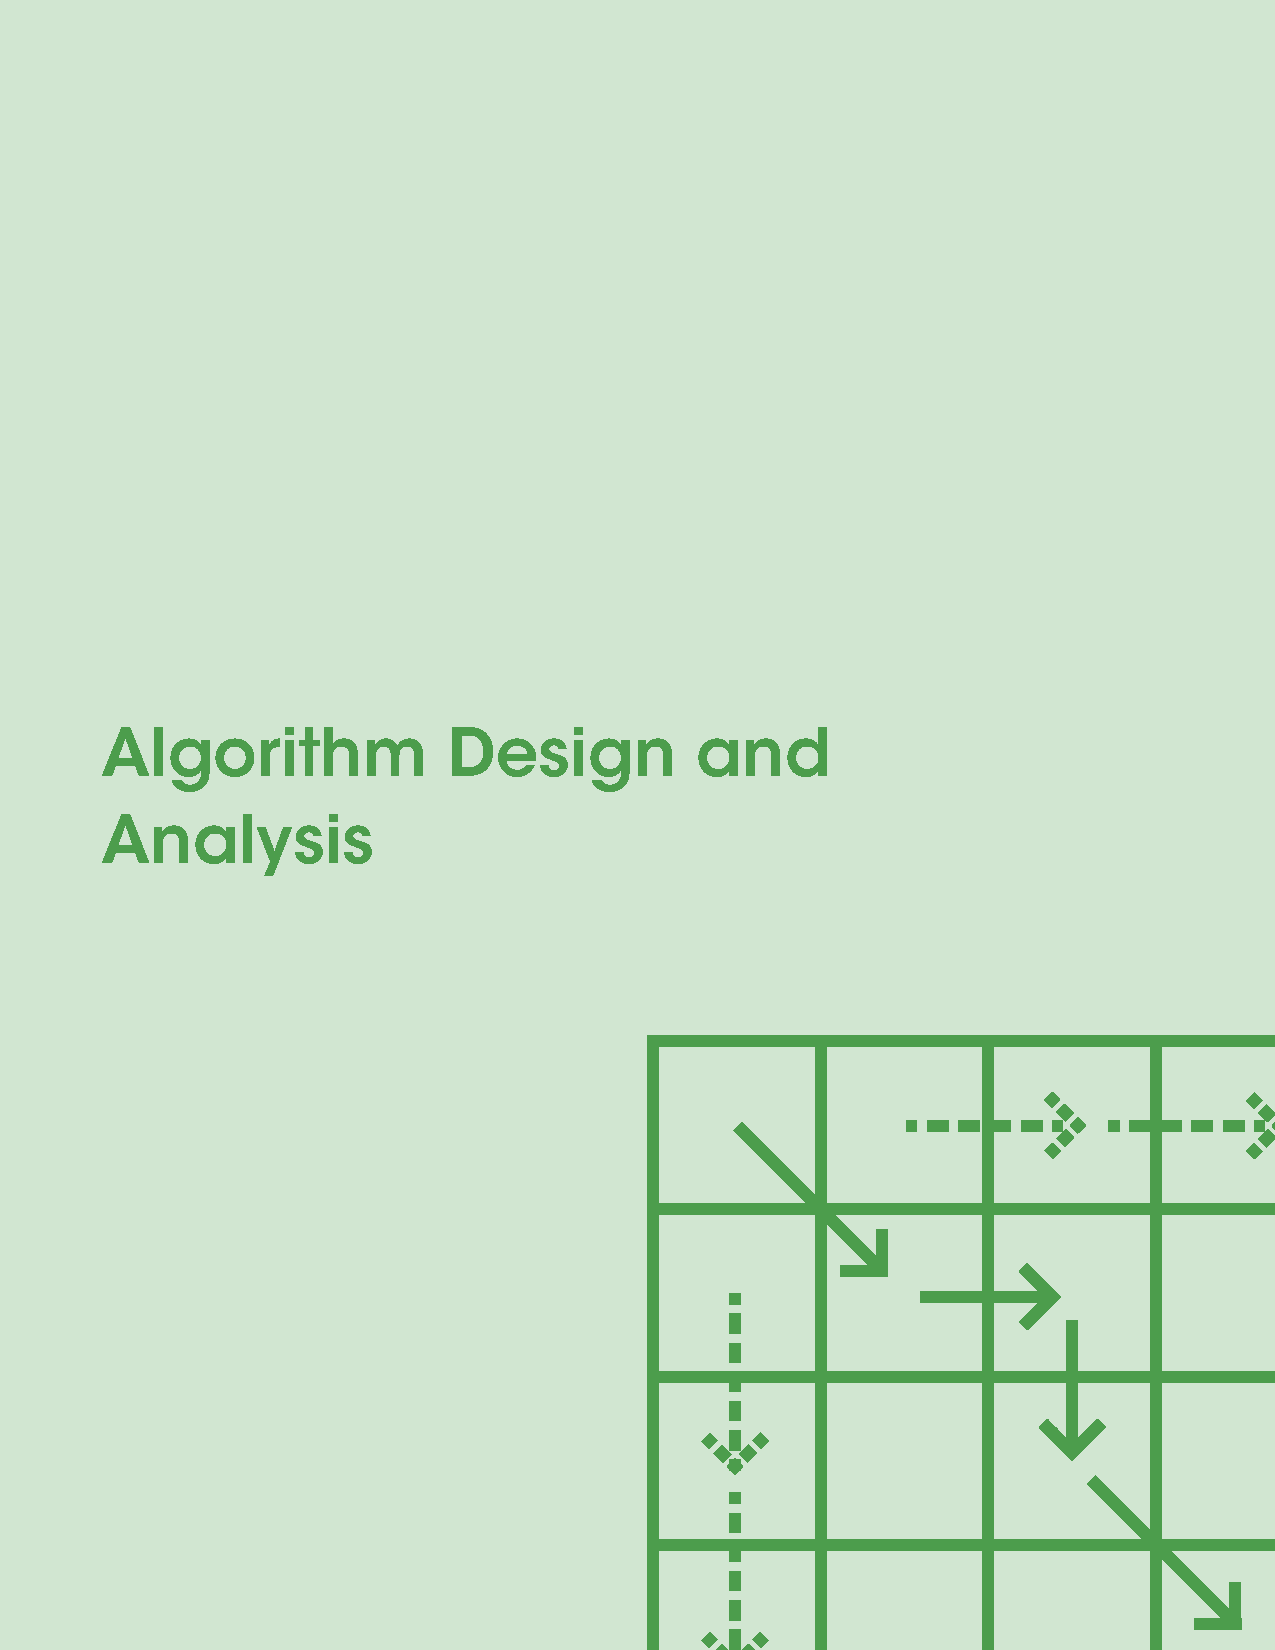
\includepdf[pages=-]{algo_cover.pdf}

%----------------------------------------------------------------------------------------
%	COPYRIGHT PAGE
%----------------------------------------------------------------------------------------

\newpage
The cover depicts a dynamic programming matrix used in the edit distance algorithm. Variations of this algorithm such as the Needleman-Wunsch and Smith-Waterman algorithms are frequently used in computational biology to align DNA or protein sequences.
~\vfill
\thispagestyle{empty}

\noindent Copyright \copyright\ \the\year{} Kevin Gao % Copyright notice

\hfill

\noindent \textsc{terra-incognita.dev} % URL

\hfill

% License information
\noindent Licensed under the Creative Commons Attribution-NonCommercial 3.0 Unported License (the ``License''). You may not use this file except in compliance with the License. You may obtain a copy of the License at \url{http://creativecommons.org/licenses/by-nc/3.0}. Unless required by applicable law or agreed to in writing, software distributed under the License is distributed on an \textsc{``as is'' basis, without warranties or conditions of any kind}, either express or implied. See the License for the specific language governing permissions and limitations under the License.


%----------------------------------------------------------------------------------------
%	TABLE OF CONTENTS
%----------------------------------------------------------------------------------------

%\usechapterimagefalse % If you don't want to include a chapter image, use this to toggle images off - it can be enabled later with \usechapterimagetrue

 % Table of contents heading image

\pagestyle{empty} % Disable headers and footers for the following pages
\usechapterimagefalse
\tableofcontents % Print the table of contents itself

\cleardoublepage % Forces the first chapter to start on an odd page so it's on the right side of the book

\pagestyle{fancy} % Enable headers and footers again

%----------------------------------------------------------------------------------------
%	PART
%----------------------------------------------------------------------------------------
\setlength{\parskip}{1em}

\part{Divide and Conquer}

\chapter{Divide and Conquer Primer}
\section{Divide and Conquer Paradigm}

Most divide and conquer algorithms follow this paradigm.

\begin{itemize}
    \item Divide up problem into several subproblems. Note that in some cases, we have to generalize the given problem.
    \item Recursively solving these subproblems.
    \item Combining the results from subproblems.
\end{itemize}

In this chapter and the following chapter, we will examine a few examples of divide-and-conquer algorithms, including but not limited to: maximum subarray, Strassen's matrix multiplication algorithm, quicksort, mergesort, median and selection in sorted array, fast Fourier transform (FTT), inversion counting, etc.

\section{The Master Theorem} \index{Master Theorem}

We have used the Master Theorem many times in both the introduction to theory of computation and data structure courses. We will once again present the theorem as it appears in CLRS here. For a careful proof of the theorem, see Section 4.6 of CLRS or Tutorial 7 note for CSC240 (Enriched Introduction to Theory of Computation).

\begin{theorem}[The Master Theorem]
    Let $a\geq 1$ and $b>1$ be constants, and let $f(n)$ be a function. Let $T(n)$ on the nonnegative integers by the recurrence
    $$
    T(n) = aT\left( \frac{n}{b} \right) + f(n)
    $$
    where $\frac{n}{b}$ is interchangeable with $\left\lfloor n/b \right\rfloor$ and $\left\lceil n/b \right\rceil $. Then, $T(n)$ has the following asymptotic bounds:
    \begin{itemize}
        \item If $f(n) \in O(n^{\log_b a - \epsilon})$ for some constant $\epsilon > 0$, then $T(n) \in \Theta(n^{\log_b a})$.
        \item If $f(n) \in \Theta(n^{\log_b a})$, then $T(n) \in \Theta(n^{\log_b a} \lg n)$.
        \item If $f(n) \in \Omega(n^{\log_b a+\epsilon})$ for some constant $\epsilon > 0$, and if $af(n/b) \leq cf(n)$ for some constant $c < 1$ and all sufficiently large $n$, then $T(n) \in \Theta(f(n))$. 
    \end{itemize}
\end{theorem}

An equivalent formulation of the theorem is as follows.

\begin{theorem}[The Master Theorem]
    Suppose that for $n \in \Z^+$.
    \begin{equation*}
        T(n) =
        \begin{cases}
        c & \text{if $n<B$} \\
        a_1 T(\lceil n/b \rceil) + a_2 T(\lfloor n/b \rfloor) + dn^i & \text{if $n\geq B$}
        \end{cases}
    \end{equation*}
    where $a_1, a_2, B, b \in \N$.
    
    Let $a = a_1+a_2 \geq 1$, $b>1$, and $c,d,i \in \R \cup \{0\}$. Then,
    \begin{equation*}
        T(n) \in
        \begin{cases}
        O(n^i \log n) & \text{if $a=b^i$} \\
        O(n^i) & \text{if $a < b^i$} \\
        O(n^{\log_b a}) & \text{if $a > b^i$}
        \end{cases}
    \end{equation*}
\end{theorem}

\section{Counting Inversions}

The objective of array inversion problems is to find the number inversions in an unsorted array compared to a sorted array. That is, given an array $A$, how many pairs $(i,j)$ are there such that $i < j$ and $A[i] > A[j]$. In other words, it counts the number of element-wise swaps needed in order to sort the given array.

For example, given the array $[8,4,2,1]$, the algorithm should answer 6 since the array has these six inversions: $(8,4)$, $(4,2)$, $(8,2)$, $(8,1)$, $(4,1)$, and $(2,1)$. If we follow these inversions, we will get a sorted array.

An naive algorithm for this problem is naturally to examine every pair of elements in the given array, which will take $O(n^2)$ comparisons. However, due to its resemblance to sorting, it is not hard to come up with a divide-and-conquer algorithm similar to mergesort that solves this problem in $O(n\log n)$ time.

At a high level, the algorithm should follow the aforementioned paradigm:
\begin{itemize}
    \item Divide: split list into two halves $A$ and $B$ 
    \item Conquer: recursively count inversions in each list
    \item Combine: count inversions $(a,b)$ with $a \in A$ and $b \in B$ 
    \item Return the sum of the tree counts
\end{itemize}

For the combine step, we assume that the two subarrays $A$ and $B$ are sorted. Then, we can scan $A$ and $B$ from left to right in parallel and compare $A[i]$ and $B[j]$. If $A[i] < B[j]$, then $A[i]$ is not inverted with any element in $B$. If $A[i] > B[j]$ then $B[j]$ is inverted with every element in left in $A$.

A pseudocode for the algorithm is shown below. Equivalently, instead of explicitly splitting the array, we can perform this in place by passing around the indices $p$ and $q$, as shown in Section 2.3.1 of CLRS.

\begin{codebox}
    \Procname{$\proc{Sort-And-Count}(L)$}
    \li \If $\attrib{L}{length} \isequal 0$ \Then
        \li \Return $(0,L)$ 
        \End
    \li $\id{mid} = \lfloor (1 + \attrib{L}{length})/2  \rfloor$
    \li $(\id{count-a}, A) = \proc{Sort-And-Count}(A[1\ldots \id{mid}])$
    \li $(\id{count-b}, B) = \proc{Sort-And-Count}(A[\id{mid}+1 \ldots \attrib{A}{length}])$ 
    \li $(\id{count-ab}, L') = \proc{Merge-And-Count}(A,B)$
    \li \Return $(\id{count-a}+\id{count-b}+\id{count-ab}, \, L')$ 
\end{codebox}

\begin{codebox}
    \Procname{$\proc{Merge-And-Count}(A,B)$}
    \li $\id{count} = 0$
    \li $i,j,k = 1$ 
    \li $L = []$ 
    \li \While $i \leq \attrib{A}{length}$ and $j \leq \attrib{B}{length}$ \Do
        \li \If $A[i] \leq B[j]$ \Then
            \li $L[k] = A[i]$
            \li $i = i + 1$
        \li \Else
            \li $\id{count} = \id{count} + 1$
            \li $L[k] = B[j]$
            \li $j = j + 1$
            \End
        \li $k = k + 1$
        \End
    \li \While $i \leq \attrib{A}{length}$ \Do
        \li $L[k] = A[i]$
        \li $k = k + 1$
        \End
    \li \While $j \leq \attrib{B}{length}$ \Do
        \li $L[k] = B[j]$
        \li $k = k + 1$
        \End
    \li \Return $(\id{count}, L)$ 
\end{codebox}

The number of comparisons made by the algorithm is given by this recurrence
$$
T(n) =
\begin{cases}
    \Theta(1) & \text{if $n = 1$} \\
    T(\lceil n/2 \rceil) + T(\lfloor n/2 \rfloor) + \Theta(n) & \text{otherwise}
\end{cases}
$$
By Masters Theorem, $T(n) \in O(n \log n)$.

\section{Closest Pair}

\vspace{\parskip}

\begin{lemma}
    Let $p$ be a point in the $2\delta$ strip within $\delta$ distance horizontally. There are at most 7 points $p$ such that $|y_p-y_q| \leq \delta$.
\end{lemma}

\begin{proof}
    $p$ must lie either in the left or right $\delta \times \delta$ square. Within each square, each point have distance at least $k$ from each other. So, we can pack at most 4 such points into one square, and since we have a left square and right square, we have 8 points in total. Other than $p$, there are at most 7 points.
\end{proof}

\begin{codebox}
    \Procname{$\proc{Closest-Pair}(P=p_1,p_2,\ldots,p_n)$}
    \li compute a vertical line $L$ such that half the points 
    \zi are on each side \RComment{$O(n \log n)$}
    \zi \Comment{consider sorting based on $x$-axis}
    \li $\delta_1 = \proc{Closest-Pair}(P_L)$
    \li $\delta_2 = \proc{Closest-Pair}(P_R)$
    \li $\delta = \min \{ \delta_1,\delta_2 \}$
    \li \For $p$ in $p_1,p_2,\ldots,p_n$ \Do \RComment{$O(n)$}
        \li \If $\proc{Y-Distance}(p,L)$ \Then
            \li \textbf{delete} $p$
        \End
    \End
    \li sort remaining points by $y$-coordinate \RComment{$O(n\log n)$}
    \li \For $p$ in $p_1,p_2,\ldots,p_n$ \Do \RComment{$O(n)$}
        \li \For $i$ \textbf{from} 1 \textbf{to} 7 \Do
            \li $p_i = \text{$i$th neighbor of $p$}$
            \li \If $\proc{Distance}(p,p_i) < \delta$ \Then
                \li $\delta = \proc{Distance}(p,p_i)$
            \End
        \End
    \End
    \li \Return $\delta$ 
\end{codebox}

The number of operations performed by this algorithm is
$$
T(n) =
\begin{cases}
    \Theta(1) & \text{if $n = 1$} \\
    T(\lceil n/2 \rceil) + T(\lfloor n/2 \rfloor) + O(n\log n) & \text{otherwise}
\end{cases}
$$
By Masters Theorem, $T(n) \in O(n \log^2 n)$.

\begin{theorem}[Lower Bound for Closest Pair]
    In a quadradic decision tree model, the closest pair problem requires at least $\Omega(n \log n)$ quadratic tests.
\end{theorem}

A quadradic decision tree is a comparison tree whose internal nodes are labeled with quadradic comparisons in the form of $x_i < x_j$ or $(x_i - x_k)^2 - (x_j - x_k)^2 < 0$. More generally, each internal node contains a comparison between a polynomial of degree at most 2 and 0 (2nd-order algebraic decision tree).

A hand-wavy proof of this lower bound follows by reduction from the result that the element uniqueness problem has a $\Omega(n \log n)$ lower bound, first shown by Ben-Or in \textit{Lower Bounds For Algebraic Computation Trees}. Element distinctness reduces to 2D closest pair problem.

\section{Karatsuba's Integer Multiplication Algorithm} \index{Karatsuba's algorithm}

To multiply two $n$-bit integers $a$ and $b$, we can follow this recursive procedure:
\begin{itemize}
    \item add two $\frac{1}{2}n$ bit integers
    \item multiply three $\frac{1}{2}n$-bit integers recursively
    \item add, subtract, and shift to obtain the result
\end{itemize}

$$
\begin{aligned}
    a &= 2^{n/2} a_1 + a_0 \\
    b &= 2^{n/2} b_1 + b_0 \\
    ab &= 2^n a_1b_1 + 2^{n/2} (a_1b_0 + a_0b_1) + a_0b_0 \\
    &= 2^n \underbrace{a_1b_1} + 2^{n/2} (\underbrace{(a_1+a_0)(b_1+b_0)} - \underbrace{a_1b_1} - \underbrace{a_0b_0}) + \underbrace{a_0b_0}
\end{aligned}
$$
The recursive steps are labeled with underbrace. By Masters Theorem, Karatsuba's algorithm performs
$$
T(n)=3T(\lceil n/2\rceil )+cn+d \in \Theta(n^{\log_2 3})
$$
bit-wise operations.

\chapter{Strassen's Algorithm}
\section{Matrix Multiplication}

The standard method to multiply two $n \times n$ matrices requires $O(n^3)$ scalar operations (multiplication and addition). The standard algorithm follows from the definition of matrix multiplication that the $i,j$ entry of $C=A \cdot B$ is given by
$$
c_{ij} = \sum_{k=1}^n a_{ik} \cdot b_{kj}
$$
\begin{codebox}
    \Procname{$\proc{Square-Matrix-Multiply}(A,B)$}
    \li $n = \attrib{A}{rows}$
    \li $C = \text{$n \times n$ matrix}$
    \li \For $i=1$ to $n$ \Do
        \li \For $j=1$ to $n$ \Do
            \li $c_{ij} = 0$
            \li \For $k=1$ to $n$ \Do
                \li $c_{ij} = c_{ij} + a_{ij}b_{ij}$
            \End
        \End
    \End
    \li \Return $C$ 
\end{codebox}
Clearly, this algorithm runs in $\Theta(n^3)$. 

\section{A Recursive Approach}

Without loss of generality, let $n=2^k$ for some $k$. Then, we can divide any $n \times n$ matrix into four $n/2 \times n/2$ matrices.
$$
\begin{bmatrix} C_{11} & C_{12} \\ C_{21} & C_{22} \end{bmatrix} = \begin{bmatrix} A_{11} & A_{12} \\ A_{21} & A_{22} \end{bmatrix}  \cdot \begin{bmatrix} B_{11} & B_{12} \\ B_{21} & B_{22} \end{bmatrix} 
$$
Since matrices are a non-commutative ring, $n \times n$ matrix multiplication can be realized in $7 n/2 \times n/2$ matrix multiplications and 18 matrix additions. Matrix addition only takes $O(n^2)$ scalar operations. Then, we have the following recurrence
$$
T(n) =
\begin{cases}
    1 & \text{if $n = 1$} \\
    7 T(n/2) + O(n^2) & \text{otherwise}
\end{cases}
$$
which implies that $T(n) \in O(n^{\log_2 7})$.

An implementation of this recursive approach is presented in pseudocode below
\begin{codebox}
    \Procname{$\proc{Square-Matrix-Multiply}(A,B)$}
    \li $n = \attrib{A}{rows}$
    \li $C = \text{$n\times n$ matrix}$ 
    \li \If $n \isequal 1$ \Then
        \li $c_{11} = a_{11} \cdot b_{11}$
    \Else
        \li partition $A$, $B$, and $C$ each into four sub-matrices
        \li $C_{11} = \proc{Square-Matrix-Multiply}(A_{11},B_{11}) + $
        \zi \> $\phantom{=}\proc{Square-Matrix-Multiply}(A_{12},B_{21})$
        \li $C_{12} = \proc{Square-Matrix-Multiply}(A_{11},B_{12}) + $
        \zi \> $\phantom{=}\proc{Square-Matrix-Multiply}(A_{12},B_{22})$
        \li $C_{21} = \proc{Square-Matrix-Multiply}(A_{21},B_{11}) + $
        \zi \> $\phantom{=}\proc{Square-Matrix-Multiply}(A_{22},B_{21})$
        \li $C_{22} = \proc{Square-Matrix-Multiply}(A_{21},B_{12}) + $
        \zi \> $\phantom{=}\proc{Square-Matrix-Multiply}(A_{22},B_{22})$
    \End
    \li \Return $C$ 
\end{codebox}
However, this particular implementation of the recursive approach still has a $O(n^3)$ running time, as demonstrated by solving the recurrence by Masters Theorem.

\section{Strassen's Algorithm}

Strassen's algorithm is a rather peculiar algorithm that multiplies two square matrices using $O(n^{\log_2 7}) = O(n^{2.81})$ scalar operations. It is debatable how practical asymptotically faster matrix multiplication algorithms (including Strassen's algorithm and Coppersmith-Winograd algorithm) are given that their crossover point (the threshold on input size beyond which such algorithms become actually faster) is often quite large for them to be useful in practical applications.

Strassen's algorithm as described in CLRS works as follows:
\begin{enumerate}
    \item Divide the input matrices $A$ and $B$ and output matrix $C$ into $n/2 \times n/2$ submatrices. This takes $\Theta(1)$ operations.
    \item Create 10 submatrices $S_1,S_2,\ldots,S_{10}$, each of which is $n/2 \times n/2$ and is the sum or difference of two matrices created in Step 1. This can be done in $\Theta(n^2)$.
    \item Using the submatrices in Step 1 and the 10 matrices in Step 2, recursively compute seven matrix products $P_1,P_2,\ldots,P_7$. Each matrix $P_i$ is $n/2 \times n/2$.
    \item Compute the desired $C_{11},C_{12},C_{21},C_{22}$ of the result matrix $C$ by adding and subtracting various combinations of the $P_i$ matrices. This can also be done in $\Theta(n^2)$ time.
\end{enumerate}
More specifically, in Step 2,
$$
\begin{aligned}
    S_1 &= B_{12} - B_{22} \\
    S_2 &= A_{11} + A_{12} \\
    S_3 &= A_{21} + A_{22} \\
    S_4 &= B_{21} - B_{11} \\
    S_5 &= A_{11} + A_{22} \\
    S_6 &= B_{11} + B_{22} \\
    S_7 &= A_{12} - A_{22} \\
    S_8 &= B_{21} + B_{22} \\
    S_9 &= A_{11} - B_{21} \\
    S_{10} &= B_{11} + B_{12},
\end{aligned}
$$
and in Step 3,
$$
\begin{aligned}
    P_1 &= A_{11} \cdot S_1 &=& A_{11} \cdot B_{12} - A_{11} \cdot B_{22} \\
    P_2 &= S_2 \cdot B_{22} &=& A_{11} \cdot B_{22} + A_{12} \cdot B_{22} \\
    P_3 &= S_3 \cdot B_{11} &=& A_{21} \cdot B_{11} + A_{22} \cdot B_{11} \\
    P_4 &= A_{22} \cdot S_4 &=& A_{22} \cdot B_{21} - A_{22} \cdot B_{11} \\
    P_5 &= S_5 \cdot S_6 &=& A_{11} \cdot B_{11} + A_{11} \cdot B_{22} + A_{22} \cdot B_{11} + A_{22} \cdot B_{22} \\
    P_6 &= S_7 \cdot S_8 &=& A_{12} \cdot B_{21} + A_{12} \cdot B_{22} - A_{22} \cdot B_{21} - A_{22} \cdot B_{22} \\
    P_7 &= S_9 \cdot S_{10} &=& A_{11} \cdot B_{11} + A_{11} \cdot B_{12} - A_{21} \cdot B_{11} - A_{21} \cdot B_{12}.
\end{aligned}
$$
In Step 4,
$$
\begin{aligned}
    C_{11} &= P_5 + P_4 - P_2 + P_6 \\
    C_{12} &= P_1 + P_2 \\
    C_{21} &= P_3 + P_4 \\
    C_{22} &= P_5 + P_1 - P_3 - P_7
\end{aligned}
$$

\chapter{Fast Fourier Transform}
\section{Motivation}
A polynomial can be represented in various ways. Each representation has its advantages and downsides.

In general, a polynomial $A(x)$ of degree $n-1$ can be written as
$$
\begin{aligned}
    A(x) &= a_0 + a_1x + a_2x^2 + \cdots + a_{n-1}x^{n-1} \\
    &= \sum_{k=0}^{n-1} a_k x^k
\end{aligned}
$$

\subsection{Coefficient Vector}

For a polynomial $A(x)$ of degree $n-1$, the coefficient vector contains the coefficient of the polynomial represented as a vector.
$$
A(x) = a_0 + a_1 x + a_2 x^2 + \cdots + a_{n-1}x^{n-1} \quad  \leftrightarrow \quad \langle a_0,a_1,a_2,\ldots,a_{n-1} \rangle
$$

\subsection{Roots}

Equivalently,
$$
A(x) = (x-r_0) (x-r_1) \cdots (x - r_{n-1}) \cdot c
$$
where $r_0,r_1,\ldots,r_{n-1}$ are the $n$ roots of the polynomial and $c$ is a scale term.

\subsection{Samples}

Given a polynomial, we can take $n$ points (coordinates): 
$$
(x_0,y_0),\, (x_1,y_1),\, \ldots ,\, (x_{n-1},y_{n-1})
$$
where $A(x_i)=y_i$ for all $i \in \{0,1,\ldots,n-1\}$. This representation is also known as the point-value representation.

By the Foundamental Theorem of Algebra, these samples uniquely define a polynomial of degree $n-1$.

\begin{theorem}[The Fundamental Theorem of Algebra]
    A univariate polynomial of degree $n$ with complex coefficients has exactly $n$ complex roots.
\end{theorem}

\begin{corollary}[Uniqueness of Polynomial Interpolation]
    A degree $n-1$ univariate polynomial $A(x)$ is uniquely defined by its evaluation at $n$ distinct values of $x$.
\end{corollary}

\section{Operations on Polynomials}

There are three primary operations on polynomials: evaluation, addition, and multiplication. The complexity of these operations varies depending on the representation. There is not a single representation that is efficient for all operations, so we need a way to efficiently convert between the representations. 

\subsection{Coefficient Representation}

\subsubsection{Evaluation}

Evaluation is efficient when the polynomial is represented as the coefficient vector using the Horner's rule:
$$
A(x_0) = a_0 + x_0 (a_0 + x_0 (a_2 + \cdots + x_0 (a_{n-2} + x_0 (a_{n-1})) \cdots ))
$$
which can be written in pseudocode as follows
\begin{codebox}
    \Procname{$\proc{Evaluate}(A=\langle a_0,\ldots a_{n-1}\rangle,\,x)$}
    \li $y = 0$
    \li \For $i = n-1$ \textbf{to} 0 \Do
        \li $y = a_j + (x \cdot y)$
    \End
    \li \Return $y$ 
\end{codebox}

\subsubsection{Addition}

Addition is easy in coefficient representation. We simply add each coefficient to get a new coefficient vector.

\begin{codebox}
    \Procname{$\proc{Add}(A=\langle a_0\ldots a_{n-1} \rangle,\, B=\langle b_0 \ldots b_{n-1} \rangle)$}
    \li \For $j = 0$ \textbf{to} $n-1$ \Do
        \li $c_j = a_j + b_j$
    \End
    \li \Return $C = \langle c_0,\ldots,c_{n-1} \rangle$
\end{codebox}

\subsubsection{Multiplication}

Multiplication is a little bit trickier in coefficient representation. We need to use linear convolution, which takes $O(n^2)$ operations.
$$
A(x) \times B(x) = \sum_{j=0}^{2n-2} c_j x^j = \sum_{j=0}^{2n-2} \sum_{k=0}^j a_k b_{j-k} x^j
$$
\begin{codebox}
    \Procname{$\proc{Multiply}(A=\langle a_0\ldots a_{n} \rangle,\, B=\langle b_0 \ldots b_{m} \rangle)$}
    \li \For $j = 0$ to $n+m$ \Do
        \li $c_j = 0$
    \End
    \li \For $j = 0$ to $n$ \Do
        \li \For $k = 0$ to $n$ \Do
            \li $c_{j+k} = c_{j+k} + a_j \cdot b_k$
        \End
    \End
    \li $C = \langle c_0 \ldots c_{n+m} \rangle$
\end{codebox}

\subsection{Samples}

\subsubsection{Evaluation}

Evaluation can be done in $O(n^2)$ through interpolation using Lagrange's formula.
$$
A(x) = \sum_{k=0}^{n-1} y_k \frac{\prod_{j\neq k} (x-x_j)}{\prod_{j \neq k} (x_k - x_j)}
$$

\subsubsection{Addition}

Addition is also easy in samples representation.
$$
A(x) + B(x):\; (x_0,y_0+z_0),(x_1,y_1+z_1),\ldots (x_{n-1},y_{n-1}+z_{n-1})
$$
given that $A(x)$ is represented as $(x_0,y_0),\ldots,(x_{n-1},y_{n-1})$ and \\ $B(x)$ is represented as $(x_0,z_0),\ldots,(x_{n-1},z_{n-1})$.

\subsubsection{Multiplication}

Multiplication is done in a similar fashion as addition.
$$
A(x) \times B(x):\; (x_0,y_0z_0),(x_1,y_1z_1),\ldots (x_{n-1},y_{n-1}z_{n-1})
$$
given that $A(x)$ is represented as $(x_0,y_0),\ldots,(x_{n-1},y_{n-1})$ and \\ $B(x)$ is represented as $(x_0,z_0),\ldots,(x_{n-1},z_{n-1})$.

\subsection{Roots}
\subsubsection{Evaluation}
Takes $O(n)$ operations by substitution and multiplication.

\subsubsection{Addition}
Impossible in the general case. There is not a general formula that can converts a coefficient vector back to the roots.

\subsubsection{Multiplication}
Multiplying two polynomials represented by their roots is equivalent to concatenate the list of roots since the resulting polynomial will have the the same roots of both polynomials.

\subsection{Summary}

\begin{table}[htpb]
    \centering
    \begin{tabular}{c|c|c|c}
    & Coefficient & Roots & Samples \\
    \hline
    Evaluation & $O(n)$ & $O(n)$ & $O(n^2)$ \\
    \hline
    Addition & $O(n)$ & $\infty$ & $O(n)$ \\
    \hline
    Multiplication & $O(n^2)$ & $O(n)$ & $O(n)$  
    \end{tabular}
    \caption{Comparison between different representations of polynomial}
    \label{tab:polynomial-rep-comparison}
\end{table}

The following chart outlines the conversions required for efficient multiplication of polynomials. The figure is taken from CLRS pp. 904.

\begin{figure}[htbp]
    \centering
    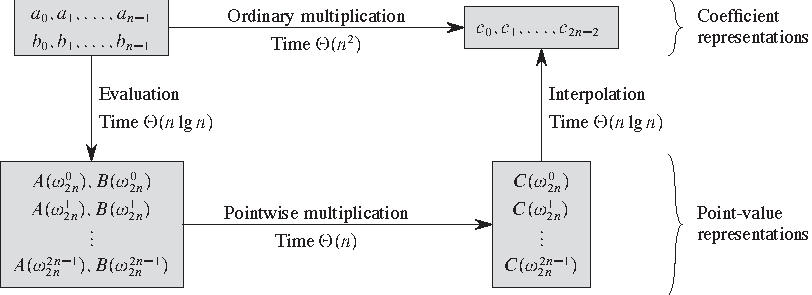
\includegraphics{fft/polynomial-conversion.pdf}
    \caption{Graphical outline of an efficient polynomial multiplication procedure.}
    \label{fig:fft-polynomial-conversion}
\end{figure}

\section{Fast Fourier Transform}

\subsection{Coefficient to Samples (and back)}

Conversion from coefficient to samples is similar to evaluation. We fix a set of points $x_0,x_1,\ldots,x_{n-1}$ and evaluate the polynomial at these points. This evaluation is equivalent to the following matrix multiplication
$$
\mathbf{y} = \mathbf{V} \mathbf{a} =
\begin{bmatrix}
1 & x_0 & x_0^2 & \cdots & x_0^{n-1} \\
1 & x_1 & x_1^2 & \cdots & x_1^{n-1} \\
1 & x_2 & x_2^2 & \cdots & x_2^{n-1} \\
\vdots & \vdots & \vdots & \ddots & \vdots \\
1 & x_{n-1} & x_{n-1}^2 & \cdots & x_{n-1}^{n-1} \\
\end{bmatrix}
\begin{bmatrix} 
    a_0 \\
    a_1 \\
    a_2 \\
    \vdots \\
    a_{n-1}
\end{bmatrix} =
\begin{bmatrix} 
    y_0 \\
    y_1 \\
    y_2 \\
    \vdots \\
    y_{n-1}
\end{bmatrix} 
$$
where $\mathbf{V}$ is called the Vandermonde matrix with entries $V_{jk} = x_j^k$ and $\mathbf{a}$ is the coefficient vector of the polynomial $A(x)$.

Evaluating this matrix product takes $\Theta(n^2)$ scalar operations. Similarly, to convert from samples back to polynomial (interpolation), we can compute $\mathbf{V}^{-1}$ using Gaussian elimination with $O(n^3)$ operations, and computing $\mathbf{a} = \mathbf{V}^{-1}\mathbf{y}$ (it is rarely a good idea to invert any matrices; ``Don't invert that matrix!'' -- John Cook).

In order to obtain efficient algorithms for manipulating polynomials, we need to somehow get rid of the $O(n^2)$ overhead resulted from the interconversion between coefficient and samples.

Note that we simply said ``fix $x_0\ldots x_{n-1}$'' when constructing the Vandermonde matrix without putting any constraints on what values of $x$ to take. By choosing special values for $x$, we can reduce the conversion overhead to $O(n \log n)$.

\subsection{Divide and Conquer}

We can formulate the evaluation $\mathbf{y}=\mathbf{V}\mathbf{a}$ as a divide and conquer algorithm.

We can come up with an outline of the algorithm by following the divide-and-conquer paradigm
\begin{enumerate}
    \item Divide: divide the polynomial $A$ into even and odd coefficients (this is equivalent to divide the coefficient vector $\mathbf{a}$ into even and odd entries)
    $$
    A_{even}(x) = \sum_{k=0}^{\lceil \frac{n}{2}-1 \rceil} a_{2k}x^k \quad \leftrightarrow \quad \mathbf{a}_{even} = \langle a_0,a_2,a_4,\ldots \rangle
    $$
    $$
    A_{odd}(x) = \sum_{k=0}^{\lfloor \frac{n}{2}-1 \rfloor} a_{2k+1}x^k \quad \leftrightarrow \quad \mathbf{a}_{odd} = \langle a_0,a_2,a_4,\ldots \rangle
    $$
    Note that the degree of the two resulting polynomials is half of the original polynomial.

    \item Conquer: recursive conquer $A_{even}(x)$ and $A_{odd}(x)$ for $x \in X^2$ where $X^2 = \{x^2 \mid x \in X\}$.
    
    \item Combine: combine the terms as follows
    $$
    A(x) = A_{even}(x^2) + xA_{odd}(x^2)
    $$
    for $x \in \mathbf{x}$.
\end{enumerate}

It is obvious that the degree of the polynomial $n$ halves, and hence the recurrence
$$
T(n,|X|) = 2T\left( \frac{n}{2},|X| \right) + O(n + |X|) \in O(n^2).
$$
This is no better than the naive approach. The main issue is that we are not halving the size of $X$. Ideally, we want $X$ to be recursively collapsing.

\subsection{Complex Roots of Unity} \index{complex roots of unity}

We can construct a collapsing set of $x$'s via square roots. If we only look at real numbers, taking the square root or squaring a number won't give you fewer or more numbers, but if we broaden our view to complex numbers, we notice that starting from 1, every time we take the square root, the size of the set doubles. The $n$th root of 1 is called the \textit{\textbf{complex $n$th root of unity}}. The observation implies that if we start from the $n$th root of unity and square the elements in the set, the set will collapse every time we square it.

Example: $\{1\} \to \{1,-1\} \to \{1,-1,i,-i\} \to \{1,-1,i,-i,\pm \frac{\sqrt{2}}{2}(1+i),\pm \frac{\sqrt{2}}{2}(-1+i) \}$

The complex roots of unity are spaced equally around the unit circle centered at the origin of the complex plane. These points are of the form $\cos\theta + i\sin\theta = e^{i\theta}$ for $\theta = 0,\frac{2}{n}\pi,\frac{4}{n}\pi,\ldots,\frac{2(n-1)}{n}\pi$. 

\begin{center}
    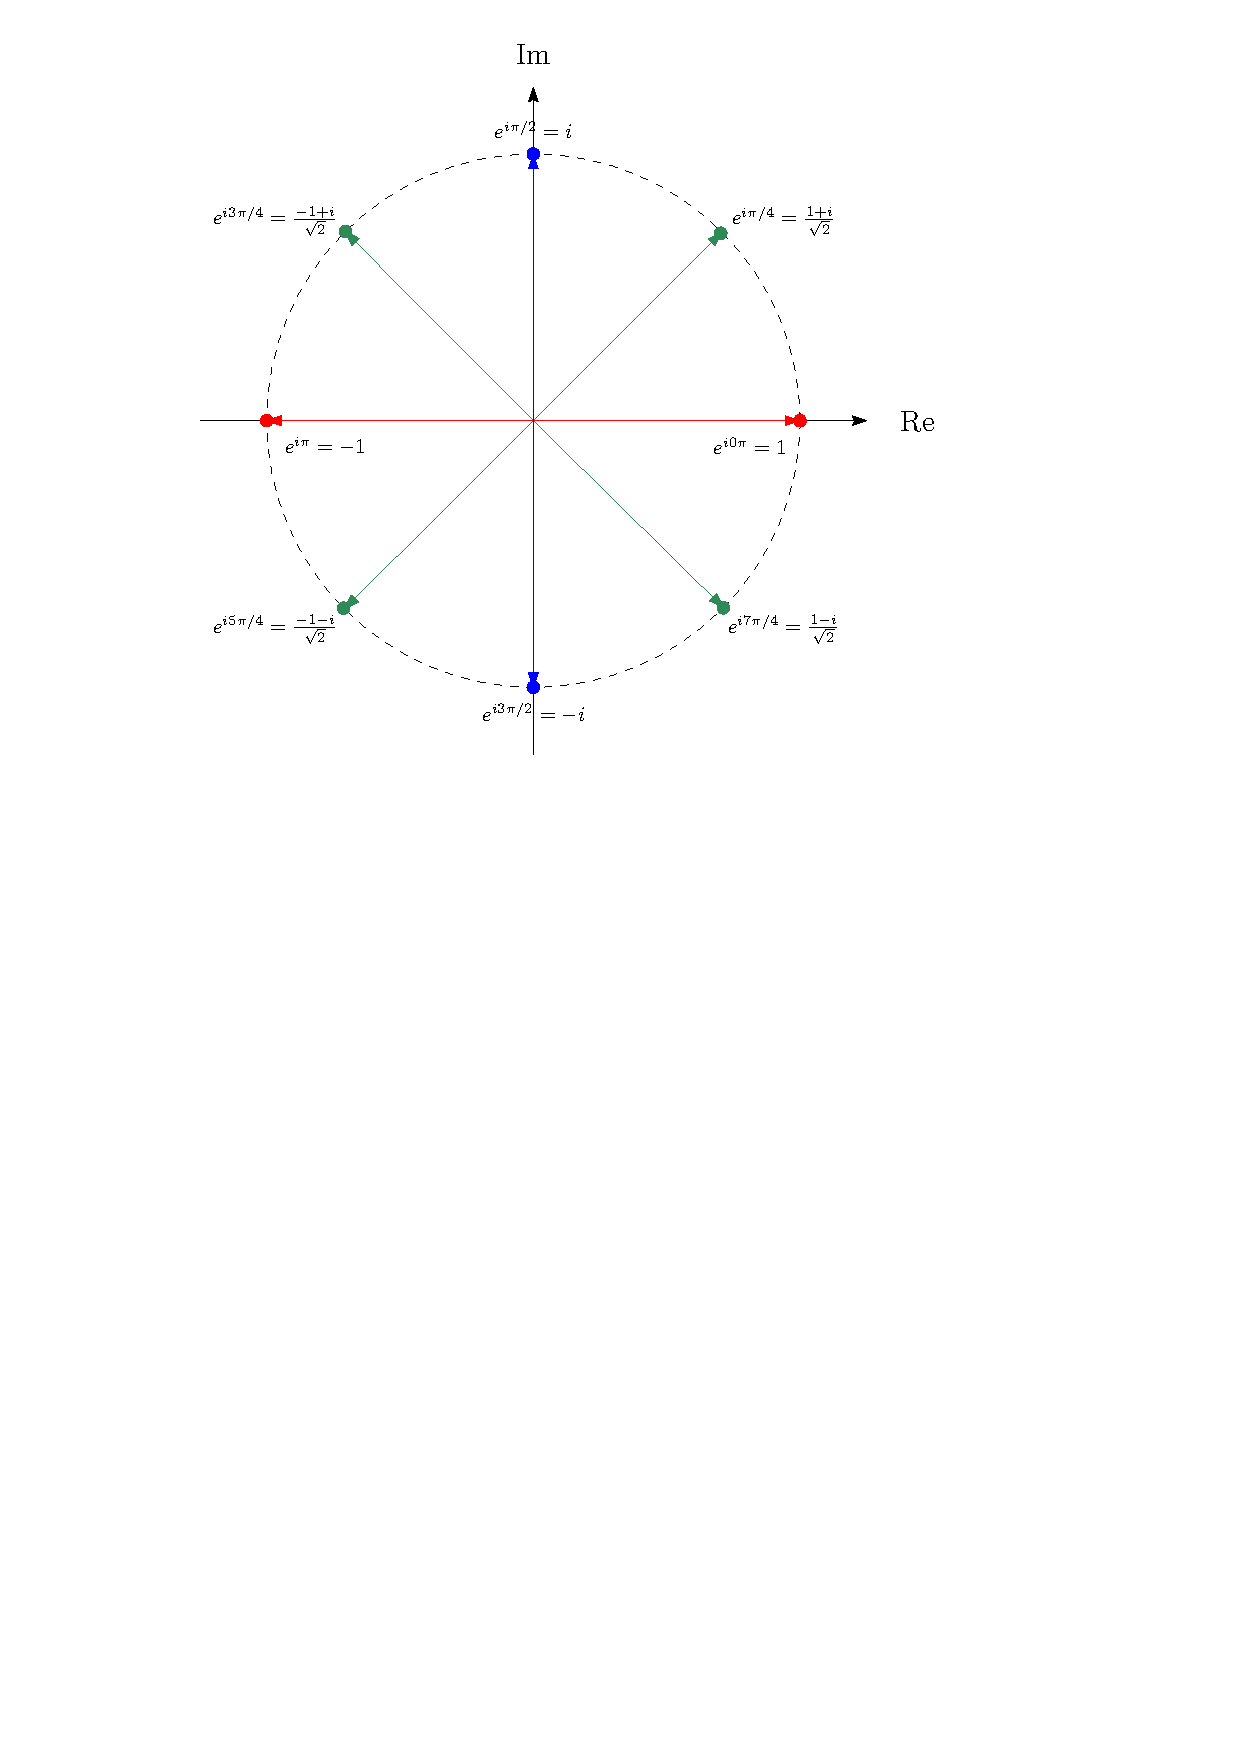
\includegraphics[width=0.6\linewidth]{fft/nth-root-of-unity.pdf}
\end{center}

The $n$th roots of unity where $n=2^\ell$ for some integer $\ell$ form a collapsing set since $(e^{i\theta})^2 = e^{i 2\theta} = e^{i(2\theta \bmod 2\pi)}$. 

Let us formalize this idea and prove that it works.

\begin{lemma}[Halving (Collapsing) Lemma]
    If $n>0$ is even, then the squares of the $n$ complex $n$th roots of unity are the $n/2$ complex $(n/2)$th roots of unity. 
\end{lemma}

\begin{proof}
    We know that $\left(e^{\frac{2\pi i}{n}}\right)^{2k} = e^{\frac{4k\pi i}{n}} = \left(e^{\frac{2\pi i}{1/2 \cdot n}}\right)^k$ for any nonnegative integer $k$. 
    
    Furthermore, $\left(e^{\frac{2\pi i}{n}}\right)^{2(k+n/2)} = \left(e^{\frac{2\pi i}{n}}\right)^{k}$. This implies that for every pair of $k$ and $k+n/2$ share the same square, and that if take the square of every element in the set of $n$th roots of unity, we get the $n/2$ elements and it follows from algebra that the resulting set contains the $(n/2)$th roots of unity.
\end{proof}

\subsection{The FFT Algorithm} \index{fast Fourier transform (FFT)}

By choosing the $x$'s in the Vandermonde matrix to be the $n$th roots of unity, we can make $X$ collapsing along with $n$. The rest of the algorithm is the same as the divide-and-conquer approach described earlier.

\begin{codebox}
    \Procname{$\proc{FFT-Recursive}(a)$}
    \li $n = \attrib{a}{length}$
    \li \If $n \isequal 1$ \Then
        \li \Return $a$ 
    \End
    \li $\omega_n = e^{2\pi i/n}$
    \li $\omega = 1$
    \li $a_{even} = (a_0,a_2,\ldots,a_{n-2})$
    \li $a_{odd} = (a_1,a_3,\ldots,a_{n-1})$
    \li $y_{even} = \proc{FFT-Recursive}(a_{even})$
    \li $y_{odd} = \proc{FFT-Recursive}(a_{odd})$
    \li \For $k = 0$ to $n/2 - 1$ \Do
        \li $y_k = y_{even}[k] + \omega y_{odd}[k]$
        \li $y_{k+\frac{n}{2}} = y_{even}[k] - \omega y_{odd}[k]$
        \li $\omega = \omega \omega_n$
    \End
    \li \Return $y = (y_0,\ldots,y_{n-1})$      
\end{codebox}

This algorithm takes $T(n) = 2T\left( \frac{n}{2} \right) + O(n) \in O(n \log n)$ operations.

\section{Inverse Fast Fourier Transform} \index{inverse fast Fourier transform (IFFT)}

The inverse discrete fourier transform is an algorithm used to find the coefficients fo a polynomial given a set of samples. The transformation is of the form $\mathbf{a}^* \to \mathbf{V}^{-1}\mathbf{a}^* = \mathbf{a}$. To evaluate this, we need $\mathbf{V}^{-1}$. In fact, this matrix has a very useful property that allows to find it without actually inverting $\mathbf{V}$ (again, don't invert the matrix).

\begin{lemma}
    Let $\mathbf{V}$ be the Vandermonde matrix constructed from the set of $n$th roots of unity. Let $\overline{\mathbf{V}}$ denote the complex conjugate of $\mathbf{V}$. Then,
    $$
    \mathbf{V}^{-1} = \frac{1}{n}\overline{\mathbf{V}}
    $$
\end{lemma}

\begin{proof}
    We claim that $\mathbf{P} = \mathbf{V}\overline{\mathbf{V}} = n \mathbf{I}$.

    Let $p_{jk}$ be the $j,k$th entry of $\mathbf{P}$.
    $$
    \begin{aligned}
        p_{jk} &= (\text{row $j$ of $\mathbf{V}$}) \cdot (\text{column $k$ of $\overline{\mathbf{V}}$}) \\
        &= \sum_{m=0}^{n-1} e^{ij2\pi m/n} \overline{e^{ik2\pi m/n}} \\
        &= \sum_{m=0}^{n-1} e^{ij2\pi m/n} e^{-ik2\pi m/n} \\
        &= \sum_{m=0}^{n-1} e^{i(j-k)2\pi m/n}
    \end{aligned}
    $$
    Take $j=k$. Then, $p_{jk} = \sum_{m=0}^{n-1} 1 = n$. Otherwise, $p_{jk} = 0$. This means that the diagonal entries are $n$, and the entires off the diagonal are all 0. Thus, the claim is true.

    It follows that $\mathbf{V}^{-1} = 1/n \mathbf{V}$.
\end{proof}

This lemma implies that for the Inverse Fast Fourier Transform algorithm, we can simply replace $e^{ikr/n}$ with its complex conjugate in the FFT algorithm and divide the final result by 2. The rest of the algorithm is analogous to that for FFT, and it is easy to see that the running of IFFT is also in $O(n \log n)$.

Quite surprisingly, many sources online including lecture notes from numerous institutions and prominant YouTube channels appear to have made some mistakes when presenting the pseudocode for IFFT. For a recursive implementation, the division by $n$ is applied only once at the very end when all recursive calls have terminated, not during the recursive call. It is not correct to simply change the twiddle factor to $w_n = e^{-2\pi i/n} / n$ or to divide by $n$ every time we update $a$ like $a_k = (a_{even}[k] + \omega a_{odd}[k])\; / n$. However, it is correct to divide by 2 every time we update $a$, as shown below. It is the same implementation as the one in Jeff Erickson's notes.

\begin{codebox}
    \Procname{$\proc{IFFT-Recursive}(y)$}
    \li $n = \attrib{y}{length}$
    \li \If $n \isequal 1$ \Then
        \li \Return $y$ 
    \End
    \li $\omega_n = e^{{\color{red}-}2\pi i/n}$
    \li $\omega = 1$
    \li $y_{even} = (y_0,y_2,\ldots,y_{n-2})$
    \li $y_{odd} = (y_1,y_3,\ldots,y_{n-1})$
    \li $a_{even} = \proc{IFFT-Recursive}(y_{even})$
    \li $a_{odd} = \proc{IFFT-Recursive}(y_{odd})$
    \li \For $k = 0$ to $n/2 - 1$ \Do
        \li $a_k = (a_{even}[k] + \omega a_{odd}[k])\; {\color{red} / \;2}$
        \li $a_{k+\frac{n}{2}} = (a_{even}[k] - \omega a_{odd}[k])\; {\color{red} / \;2}$
        \li $\omega = \omega \omega_n$
    \End
    \li \Return $a = (a_0,\ldots,a_{n-1})$      
\end{codebox}

\section{Fast Polynomial Multiplication}

With FFT, we can implement the procedure outlined in Figure \ref{fig:fft-polynomial-conversion}.

To calculate $A(x)\times B(x)$,

\begin{enumerate}
    \item Compute $A^* = \proc{FFT}(A)$ and $B^* = \proc{FFT}(B)$. This step is $O(n \log n)$.
    \item Compute $C^* = A^* \cdot B^*$ in sample representation. This step is $O(n)$.
    \item Compute $C = \proc{IFFT}(C^*)$ to get $C$ in coefficient representation. This step is $O(n \log n)$.
\end{enumerate}
Overall, the algorithm has runtime complexity of $O(n \log n)$.

\chapter{Selection in Linear Time}
\input{notes/quickselect.tex}

\part{Greedy Algorithms}

\chapter{Interval Scheduling}
\section{Interval Scheduling}

We begin by considering the interval scheduling problem. The same problem is referred to as the activity selection problem in CLRS.

Consider a set $S = \{a_1,a_2,\ldots,a_n\}$ of jobs/activities, each with a start time $s_i$ and finish time $f_i$. Two jobs are said to be compatible if they don't overlap. More formally, given activities $a_i$ and $a_j$, they are compatible if $[s_i,f_i) \cap [s_j,f_j) = \emptyset$. That is, if $s_i \geq f_j$ or $s_j \geq f_i$. The goal of the interval scheduling problem is to find a maximum-size subset of mutually compatible jobs.

Let us consider the greedy strategy for solving the interval scheduling problem. Intuitive, the globally optimal solution should leave resources/time open for as many other jobs as possible. This requires us to consider the jobs in some ``natural'' order:

\begin{itemize}
    \item Earliest start time: consider jobs in ascending order of $s_i$
    \item Earliest finish time: consider jobs in ascending order of $f_i$
    \item Shortest inverval: consider jobs in ascending order of $f_i - s_i$ 
    \item Fewest conflicts: for each job $a_i$, count the remaining number of conflicting jobs $c_i$ and schedule in ascending order of $c_i$. 
\end{itemize}

Not all of those strategies work. Here are some counterexamples (Figure \ref{fig:greedy-interval-scheduling-counterexample}).

\begin{figure}[htbp]
    \centering
    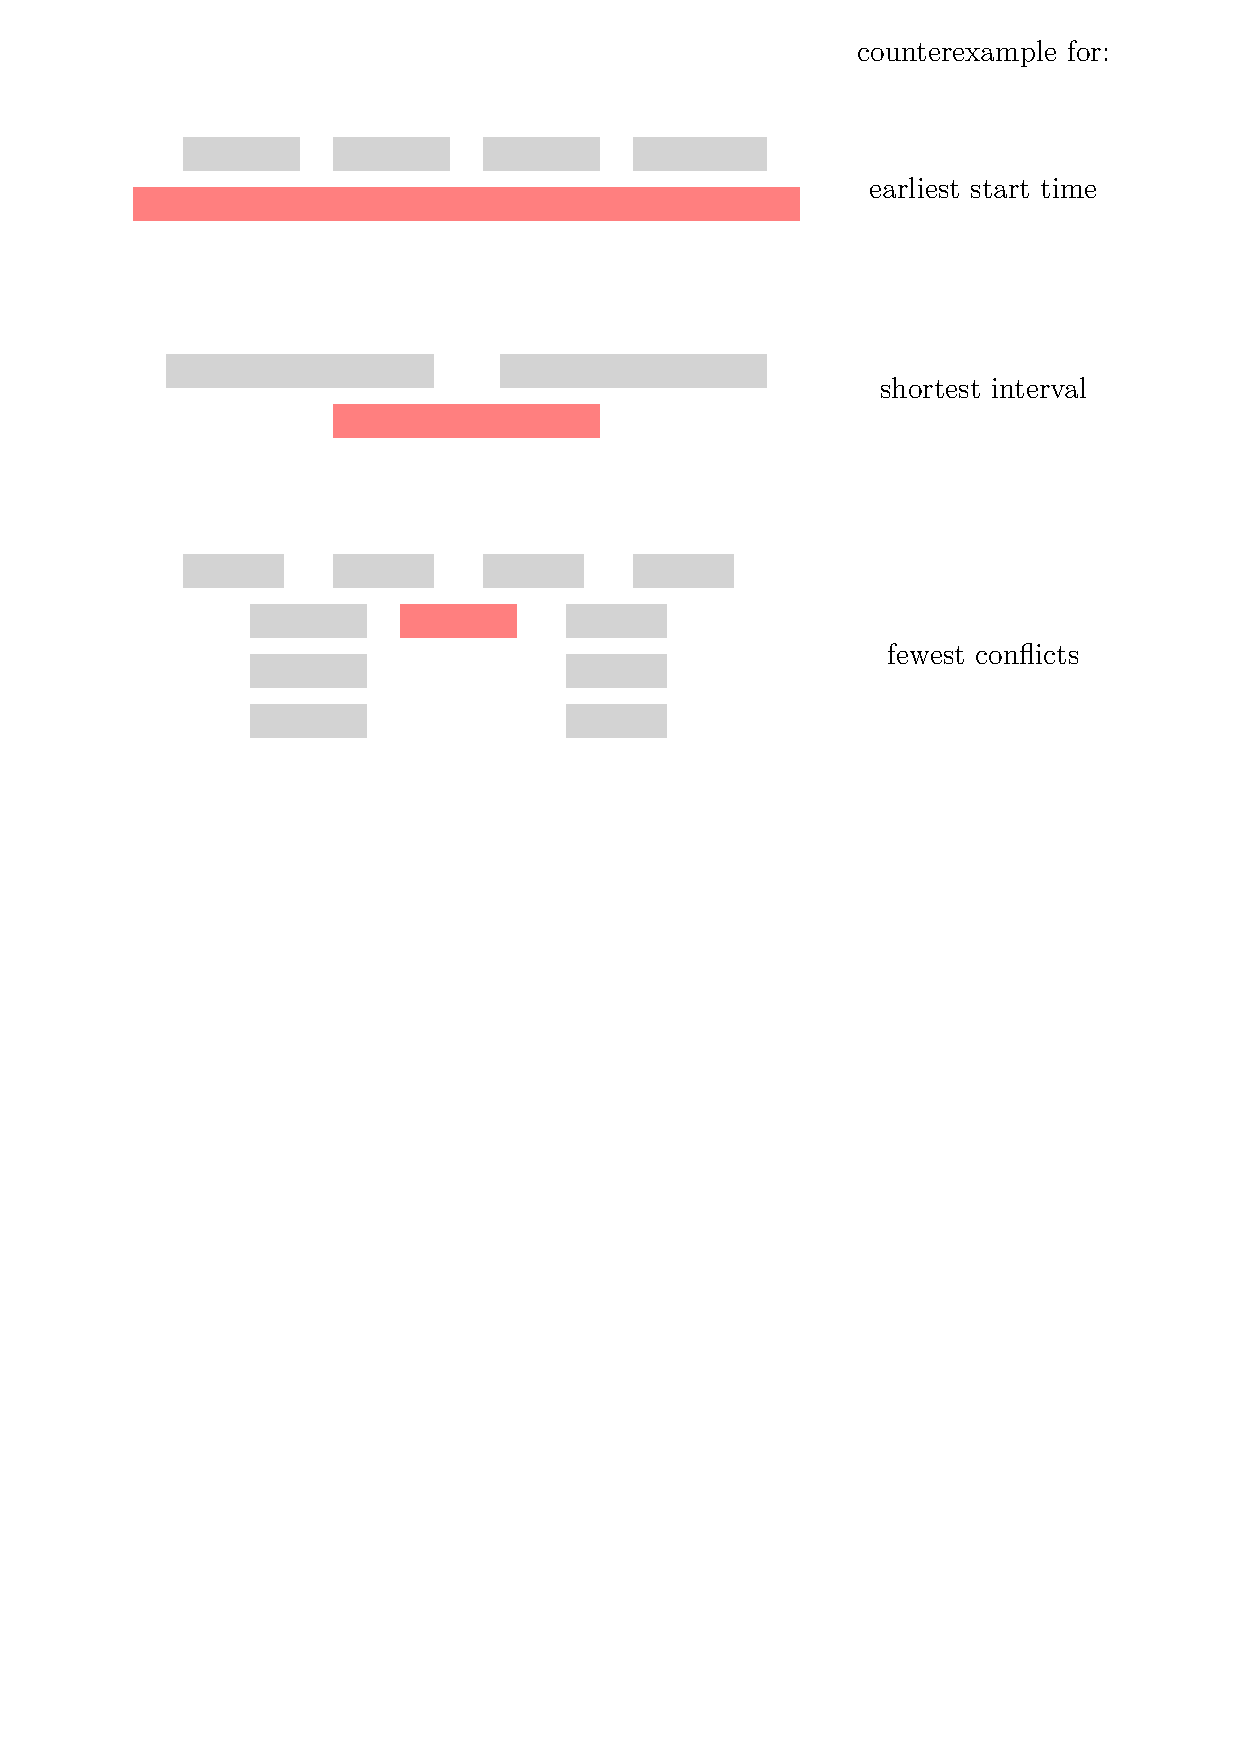
\includegraphics[width=0.7\linewidth]{greedy/interval-scheduling-counterexample.pdf}

    \hfill

    \caption{Counterexamples for the greedy strategies that do not work for the interval scheduling problem. The interval that satisfies the greedy strategy but leads to incorrect global solution is highlighted in red.}
    \label{fig:greedy-interval-scheduling-counterexample}
\end{figure}

Therefore, we choose earliest finish time as our greedy strategy, which we can implement into this recursive algorithm

\begin{codebox}
    \Procname{$\proc{Interval-Scheduling-Recursive}(S,k,n)$}
    \li $m = k + 1$
    \li \While $m \leq n$ and $S[m].s < S[k].f$ \Do
        \li $m = m + 1$
    \End
    \li \If $m \leq n$ \Then
        \li \Return $\{S[m]\} \cup \proc{Interval-Scheduling-Recursive}(S,m,n)$
    \li \Else
        \li \Return $\emptyset$ 
\end{codebox}

As a precondition, we assume that the array of jobs $S$ is sorted in monotonically increasing order by finish time. $S[i].s$ denotes the starting time of the $i$th job, and $S[i].f$ denotes the finish time of the $i$th job. $k$ is the job being considered. In each call to the recursive algorithm, we starts from $m = k+1$ and increment $m$ until we find a job with starting time $S[m].s$ strictly lower than the finish time of $S[k]$. This is the job that is selected by our greedy strategy in the current recursive call. After finding this $m$, we return the union of $\{S[m] = a_m\}$ and the maximum-size subset of $S_m$ returned by the recursive call $\proc{Interval-Scheduling-Recursive}(S,m,n)$.

The initial call that solves the problem globally is $\proc{Interval-Scheduling-Recursive}(S,0,n)$ where $n$ is the number of jobs to be considered.

This algorithm can be easily converted into an iterative algorithm.

\begin{codebox}
    \Procname{$\proc{Interval-Scheduling}(S)$}
    \li $n = \attrib{S}{length}$ 
    \li $S' = \{a_1\}$
    \li $k = 1$
    \li \For $m = 2$ to $n$ \Do
        \li \If $S[m].s \geq S[k].f$ \Then
            \li $S' = S' \cup \{S[m]\}$
            \li $k = m$
        \End
    \End
    \li \Return $S'$ 
\end{codebox}

Sorting the array of jobs takes $O(n \log n)$ time, and going over the sorted the list and check each job's compatibility takes $O(n)$ in total.

\section{Proving Optimality}

As we have demonstrated earlier in Figure \ref{fig:greedy-interval-scheduling-counterexample}, greedy strategy does not always work. It is important for us to ensure (prove) that the locally optimal greedy choice leads to a globally optimal solution. Here, we will present three equally valid proofs for the optimality of the greedy algorithm for the interval scheduling problem.

\begin{theorem}
    The greedy algorithm using earliest finish time is optimal. More formally, the algorithm returns a maximum-size set of disjoint jobs $\{a_1,\ldots,a_m\} \subseteq S$
\end{theorem}

\begin{proof}[Proof (by contradiction)]
    Suppose, for contradiction, that the greedy algorithm using earlies finish time is not optimal. Let $i_1,i_2,\ldots,i_k$ be the sequence of jobs selected by the algorithm, and let $j_1,j_2,\ldots,j_m$ be the correct solution where $m>k$. Let $r$ be the largest possible value such that $i_{r+1} \neq j_{r+1}$. That is, the $(r+1)$th job is the first job where the two sequences begin to differ. 

    Both $i_{r+1}$ and $j_{r+1}$ must be compatible with previous choices of $i$ and $j$, respectively. Let $i_1=j_1,i_2=j_2,\ldots,i_r=j_r,i_{r+1},j_{r+2}, \ldots, j_m$ be a new sequence of jobs. This is the optimal solution with $j_{r+1}$ replaced with $i_{r+1}$. By assumption, the greedy solution is not optimal so $j_{r+1}$ is not selected by the greedy algorithm and thus $i_{r+1} \leq j_{r+1}$. So, the new sequence of jobs is still feasible because $i_{r+1} \leq j_{r+1}$. The algorithm is still optimal because all $m$ disjoint jobs are scheduled. But then, $i_{r+1}$ is not different from $j_{r+1}$, which implies that $r$ is not the maximum value such that $i_{r+1} \neq j_{r+1}$. This is a contradiction. Therefore, the greedy algorithm is optimal.
\end{proof}

\begin{proof}[Proof (by induction)]
    Let $S_k$ be the subset of jobs selected by the greedy algorithm after considering the first $k$ jobs in increasing order of finish time. We say that $S_k \subseteq S$ is promising if it can be extended to the optimal solution ($S_k$ is part of the optimal solution). More formally, $S_k$ is promising if there exists $T \subseteq \{ a_{k+1},\, \ldots,\, a_{n}\}$ such that $O_k = S_k \cup T$ is optimal.

    We want to show that for all $k \in \{0,1,\ldots,n\}$, $S_k$ is promising.

    \textbf{Base case}: When $k=0$, $S_0=\emptyset$. The claim is vacuously true.
    
    \textbf{Inductive step}: Let $j \in \N$ be arbitrary. Suppose that the claim holds for $k = j - 1$ and that $S_{j-1}$ is promising. For $S_j$, there are two possibilities:

    (1) The greedy algorithm did not select job $a_j$ (i.e. $s_{j+1} < f_j$), so $S_j = S_{j-1}$. This implies that $a_j$ is not compatible with some job in $S_{j-1}$. Since $S_{j-1} \subseteq O_{j-1}$, $O_{j-1}$ does not include $a_j$. $O_j = O_{j-1}$ does not include $a_j$, so $S_j$ can be extended to $O_j$ and $S_j$ is promising.
    
    (2) The greedy algorithm selected job $a_j$ (i.e. $s_{j+1} \geq f_j$), so $S_j = S_{j-1} \cup \{a_j\}$. Consider the earliest job $a_r$ in $O_{j-1} - S_{j-1}$. Consider $O_j = O_{j-1} - \{a_r\} \cup \{a_j\}$. $O_j$ is still feasible since jobs in $O_{j-1}$ are disjoint, $a_r$ is the first to finish, and the finish time of $a_j$ is earlier or equal to the finish time of $a_r$. Hence, $S_j$ can be extended to $O_j$.

    \begin{center}
        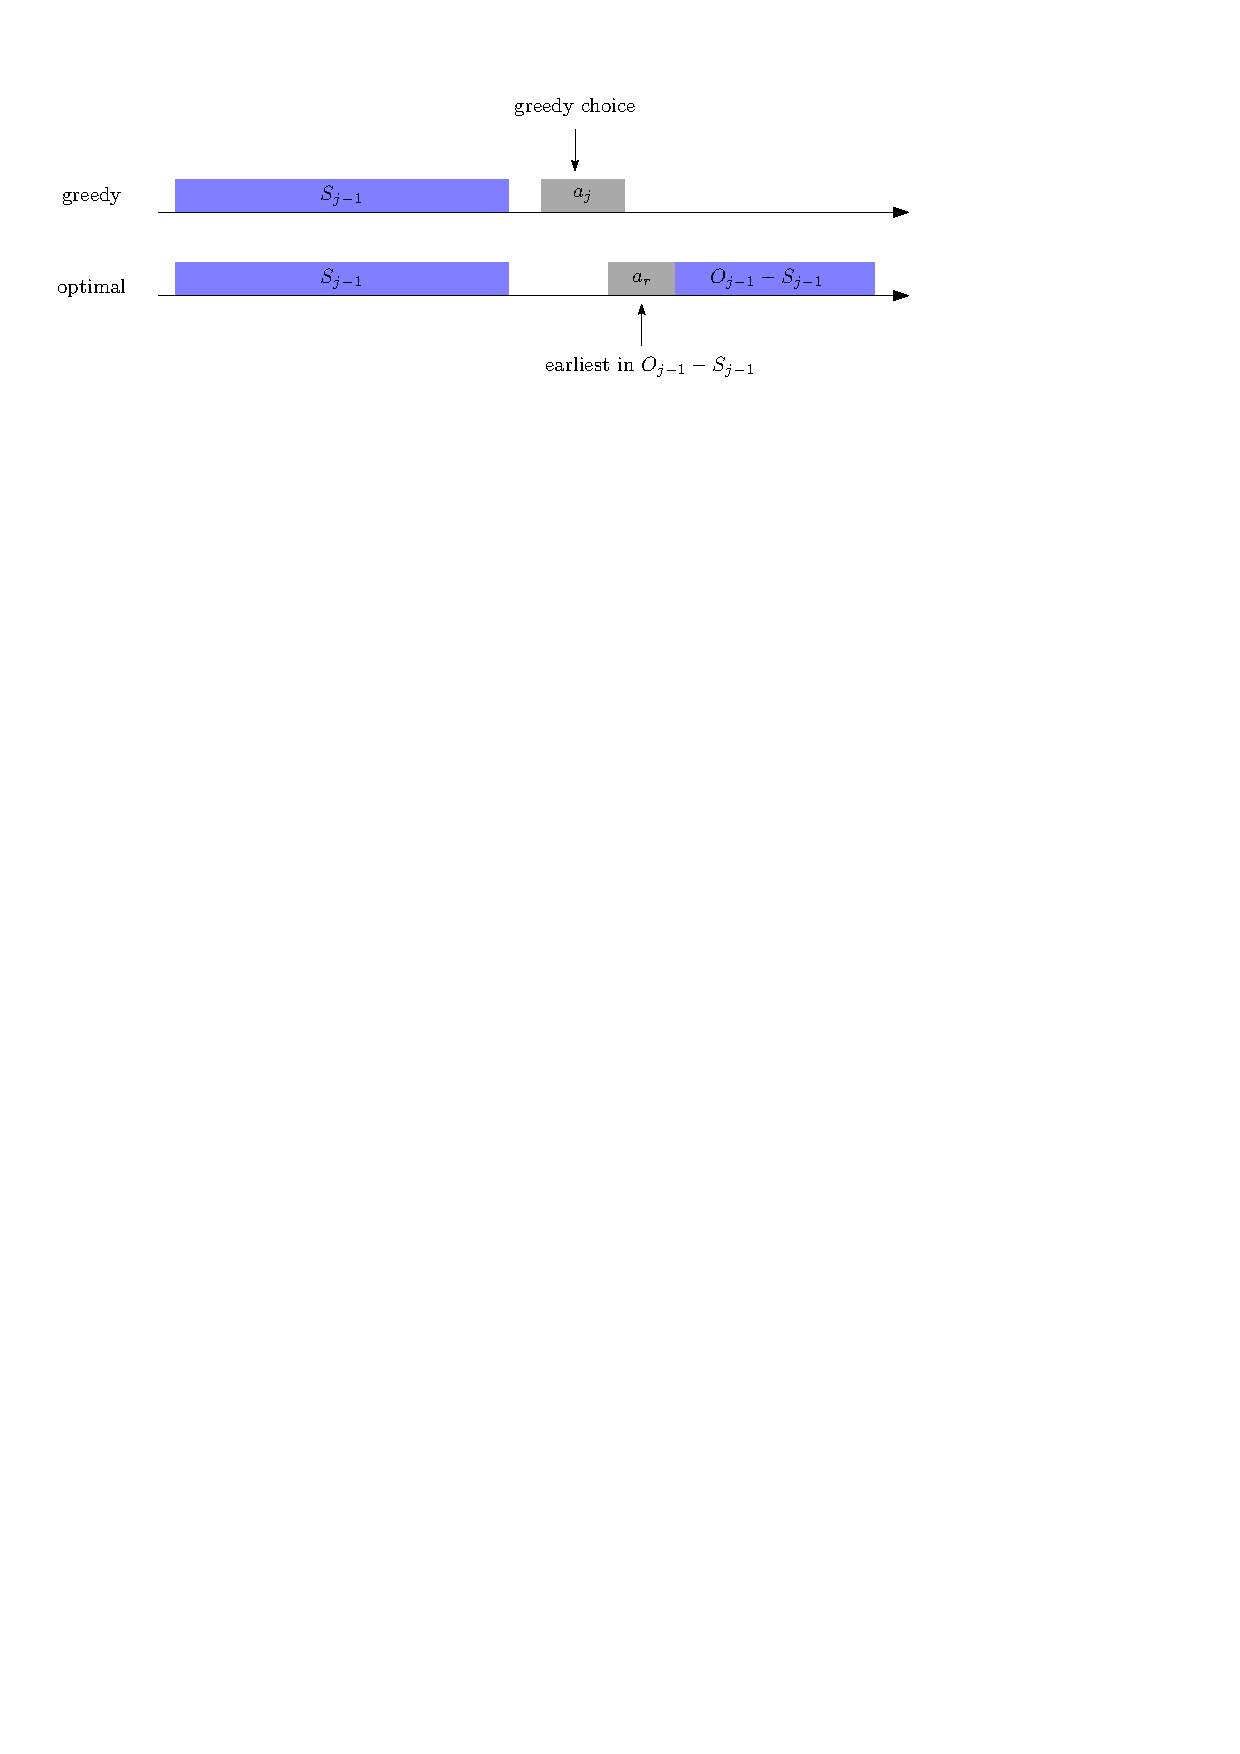
\includegraphics[width=0.7\linewidth]{greedy/interval-scheduling-optimality-proof.pdf}
    \end{center}
    By induction, the claim is true for all $k \in \{0,1,\ldots,n\}$.
\end{proof}

The previous two proofs use the technique known as the exchange argument. They both rely on the argument that if the greedy solution after $j$ iterations can be extended to an optimal solution, then the greedy solution after $j+1$ iterations can also be extended to an optimal solution by exchanging some interval with one chosen based on the greedy strategy. 

The last proof uses what we call an ``\textbf{charging argument}''. In this case, the charging argument charges each interval of an optimal solution (or arbitrary solution) to a unique interval in the greedy solution. Charging arguments are also used in approximation algorithms (for example, to prove that an algorithm is a $k$-approximation).

\begin{proof}[Proof (by charging argument)] \index{charging argument}
    Given a set of jobs $S = \{a_1,\ldots,a_n\}$, let $O$ be an optimal solution of the interval scheduling problem. Let $S'$ be the solution given by the greedy algorithm using earliest finish time. We want to find a one-to-one function $h:\, O \to S'$. For any job $j \in O$, define $h(j)$ as the interval $j' \in S'$ that intersects $j$ and has the earliest finish time amongst intervals in $S'$ intersecting $j$.

    We claim that the $h$ is well-defined so $h(j)$ must exists for all $j$. This is proved by contradiction. Suppose, for contradiction, that there exists a $j \in O$ where $h(j)$ as we defined does not exist. By definition, this means no interval in $S'$ intersects with $j$. This implies that $j$ is compatible with every interval in $S'$, so the greedy strategy would have selected $j$ and $j$ would be part of $S'$. But then if $j \in S'$, $j$ intersects with itself. This is a contradiction. $h(j)$ \textbf{exists} for all $j \in O$. Furthermore, $h(j)$ is \textbf{unique} because all intervals in $S'$ are mutually disjoint, and every interval in $S'$ that intersects $j$ have distinct finish time.

    We then show that $h$ is \textbf{injective}, similarly by contradiction. Assume that there are two intervals $j_1,j_2 \in O$ such that $h(j_1) = h(j_2) = j' \in S'$. Without loss of generality, suppose that the finish time of $j_1$ is earlier than $j_2$. $j_1$ and $j_2$ are disjoint because they are both in $O$, which implies that $f_1 \leq s_2 < f_2$. Since $j' \in S'$, the greedy algorithm must have encountered $j'$ before $j_1$ and $j_2$. Thus, $f' \leq f_1$. But then, this implies that $f' \leq f_1 \leq s_2 < f_2$. That is, $j'$ and $j_2$ do not overlap. This is a contradiction because if they do not intersect, $h(j_2) \neq j'$. Therefore, $h$ is injective.
    
    Since there exists an one-to-one function $h:\; O \to S'$, by the charging argument, the greedy algorithm for the interval scheduling problem is optimal.
\end{proof}

More generally, we have shown that $|O| \leq |S'|$, which implies the optimality of the algorithm (that the algorithm returns the maximum-size subset).

\section{Interval Coloring (Interval Partition)}

Let us know consider a modified version of the original interval scheduling problem. Suppose that we are given a set of intervals. We want to color all intervals so that intervals with the same color do not intersect while using the minimum number of colors. This problem is also known as the interval partitioning problem.

Similar to interval scheduling, let's take a look at the few possible choices for our greedy strategy:
\begin{itemize}
    \item Earliest start time
    \item Earliest finish time
    \item Shortest interval
    \item Fewest conflicts
\end{itemize}
We can show using counterexamples that the last three heuristics, earliest finish time, shortest interval, and fewest conflicts, do not work. We will prove that the earliest start time greedy choice gives us a globally optimal solution for the interval partitioning problem.

The proof for this is somewhat similar to the charging argument that we used to prove the optimality of interval scheduling. We attempt to bound the size of the solution set in order to show that it is optimal (miminal). In the charging argument, we bound the size by showing that there exists an one-to-one function. In this proof, we will skip that part and instead bound the size directly.

\begin{lemma} \label{lem:interval-partition-upper-bound}
    Given a set of intervals, let $d$ be the maximum number of intersecting intervals at any time. The number of partitions (colors) given by any algorithms that solve the interval partitioning problem must be at least $d$.
\end{lemma}

\begin{proof}
    By contradiction.
\end{proof}

\begin{lemma} \label{lem:interval-partition-lower-bound}
    Let $d$ be defined as in the previous lemma. The greedy algorithm using earliest start time produces a solution with at most $d$ partitions.
\end{lemma}

\begin{proof}
    Let $d'$ be the number of partitions produced by the greedy algorithm. Suppose for contradiction that the algorithm used more than $d$ partitions. Consider the first time that the greedy algorithm used $d+1$ partitions. Suppose this happens when the algorithm is trying to assign a partition to the interval $j$. This implies that there are $d$ intervals intersecting $j$. Let $s_j$ be the starting time of $j$. These $d$ intervals must contain $s_j$. This is because all the previous $d$ intervals have starting time earlier than $s_j$. So it must be that case that $s_j$ is after or at the starting time of the other $d$ intervals. But then, this implies that there are $d+1$ overlapping intervals at $s_j$, contradicting the fact that there are at most $d$ intersecting intervals at any time.
\end{proof}

\begin{corollary}
    The greedy algorithm produces a solution with exactly $d$ partitions.
\end{corollary}

\begin{proof}
    Follows immediately from the Lemma \ref{lem:interval-partition-upper-bound} and \ref{lem:interval-partition-lower-bound}.
\end{proof}

Hence the theorem:

\begin{theorem}
    The greedy algorithm using earliest starting time as greedy choice is optimal.
\end{theorem}

This greedy algorithm is implemented as follows. Suppose, as a precondition, that $S$ is sorted in increasing order of starting time, and that elements in $Q$ contains objects of $\proc{Interval}$s that are indexed by finish time.

\begin{codebox}
    \Procname{$\proc{Interval-Partitioning}(S)$}
    \li $d = 0$
    \zi \Comment{initialize PQ using finish time as key} 
    \li $Q = \proc{Priority-Queue}(\id{key}=f)$ 
    \li \For $i = 1$ \textbf{to} $\attrib{S}{length}$ \Do
        \li $k = \proc{Extract-Min}(Q)$
        \li \If $k \isequal \const{nil}$ \Then
            \li $d = d + 1$
            \li $\id{interval} = $ \textbf{new} $\proc{Interval}(i.f)$ 
            \li $\proc{Insert}(Q,\id{interval})$
        \End
        \li \If $i.s > \proc{Min}(Q)$ \Then
            \zi \Comment{if $i$ is compatible with $k$, allocate $i$ to $k$}
            \li $k.f = i.f$
            \li $\proc{Insert}(Q, k)$
        \li \Else
            \zi \Comment{otherwise, create new classroom $d+1$}
            \li $d = d + 1$
            \li $\proc{Insert}(Q, k)$
            \li $\id{interval} = $ \textbf{new} $\proc{Interval}(i.f)$
            \li $\proc{Insert}(Q,\id{interval})$
        \End
    \End
    \li \Return $d$
\end{codebox}

This algorithm runs in $O(n \log n)$ time. This is the case regardless of whether or not we consider sorting as part of the algorithm because the $n$ priority queue operation is going to cost $O(n \log n)$ anyway, assuming the priority is implemented as a min-heap.

\section{Greedy Strategy}

The greedy strategy can be generalized as follows:

\begin{enumerate}
    \item Cast the optimization problem as one in which we make a choice and are left with one subproblem to solve.
    \item Prove that there is always an optimal solution to the original problem that makes the greedy choice, so that the greedy choice is always safe.
    \item Demonstrate optimal substructure by showing (typically by contradiction or induction) that, having made the greedy choice, what remains is a subproblem with the property that if we combine an optimal solution to the subproblem with the greedy choice we have made, we arrive at an optimal solution to the original problem.
\end{enumerate}

\index{greedy property}
The important property that requires us to prove when implementing a greedy algorithm is the \textbf{greedy property}. It tells us that we can assemble a globally optimal solution from locally optimal choices. The exchange argument for the proof (the first two proofs that we have seen for interval scheduling) argues that we can modify the globally optimal solution to substitute the greedy choice for some other choice, resulting in one similar, but smaller, subproblem.

\chapter{Graph Algorithms Using Greedy}
\section{Interval Scheduling as Graph Problems}

There is a natural way to view the interval scheduling and partitioning problems as graph problems.

\index{intersection graph} \index{interval graph}
Let $I$ be a set of intervals. We can construct the \textit{\textbf{intersection graph}} $G(I) = (V,E)$ where $V=I$ and $(u,v) \in E$ if and only if the intervals corresponding to $u$ and $v$ intersect.

Any graph that is the intersection graph of a set of intervals is called an \textit{\textbf{interval graph}}. The interval scheduling and interval partition problem can be viewed as the \textit{\textbf{maximum independent set problem}} for the class of interval graphs.

\begin{definition}[Maximum Independent Set]
    Let $G=(V,E)$ be a graph. A subset $U$ of $V$ is an independent set (stable set) in $G$ if for all $u,v \in U$, $(u,v) \not\in E$.

    The maximum independent set of $G$ is an independent set of $G$ with maximum cardinality.
\end{definition}

\begin{pitfall}
    Maximal and maximum are \textit{\textbf{not}} the same. It is important to distinguish between ``maximum'' and ``maximal'' sets, and between ``minimum'' and ``minimal'' sets. A maximal set is a set that is not a proper subset of any other sets, while a maximum set is simply a set of maximum cardinality among all sets.
\end{pitfall}

\begin{figure}[htbp]
    \centering
    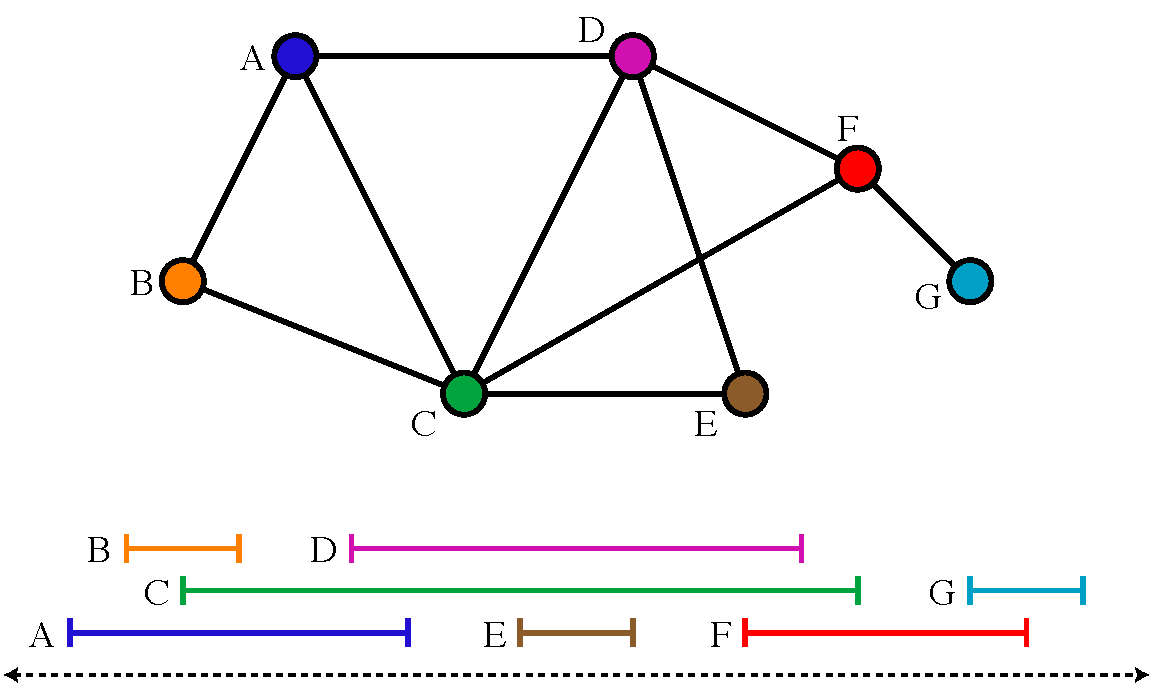
\includegraphics[width=0.6\linewidth]{greedy/Interval_graph.pdf}
    \caption{Intervals represented as an interval graph. Image from \href{https://en.wikipedia.org/wiki/Interval_graph}{Wikipedia}.}
    \label{fig:greedy-interval-graph}
\end{figure}

\begin{definition}[Graph Coloring]
    Let $G=(V,E)$ be a graph. A function $c:\, V \to \{1,\ldots,k\}$ is a valid coloring of $G$ if $c(u) \neq c(v)$ for all $(u,v) \in E$.

    The graph coloring problem is to find a coloring $c$ that minimizes the number of colors $k$. Such number is called the chromatic number of $G$, denoted $\chi(G)$.
\end{definition}

To model the interval scheduling and partition problem as a graph theory problem, we first need a way to efficiently interconvert between the interval graph representation and the set representation.

Given a set $I$ of intervals, it is easy to construct the interval graph $G(I)$. For conversion back from interval graph, the following theorem claims that it can also be done efficiently.

\begin{theorem}
    Given any graph $G$, there is a linear-time algorithm to decide if $G$ is an interval graph, and if so, to construct an interval representation.
\end{theorem}

The maximum independent set problem for intersection graph can be efficiently solved, so the interval scheduling and partition problem can also be efficiently solved. The graph theoretical explanation for this is that interval graphs are chordal graphs with a perfect elimination ordering, making it possible to use the greedy approach (or more generally, a priority based approach). However, in the general case, the maximum independent set problem is known to be NP-hard.

To formallly prove that the maximum independent set problem can be efficiently solved for interval graphs, we need to introduce a few additional concepts.

\subsection{Interval Graph is Chordal Graph}

We first show that an interval graph is also a chordal graph (the converse is not true).

\begin{definition}[Chordal Graph] \index{chordal graph} \index{rigid circuit graph} \index{chord}
    Let $G$ be an undirected graph. $G$ is a \textit{\textbf{chordal graph}} or \textit{\textbf{rigid circuit graph}} if for any cycles of 4 or more vertices, there exists a pair of vertices $u,v$ on the cycle such that $\{u,v\} \in E$ but $\{u,v\}$ is not part of the cycle. The edge $\{u,v\}$ is called a \textit{\textbf{chord}} of the cycle.
\end{definition}

\vspace{\parskip}

\begin{theorem}
    An interval graph is also a chordal graph.
\end{theorem}

\begin{proof}
    Let $G=(V,E)$ be an interval graph with a cycle $C_k = v_1v_2\ldots v_kv_1$ where $k \geq 4$ and each $v_i$ represents an interval $[a_i,b_i)$. The case where $k < 4$ is vacuously true. Suppose the first $k$ vertices of the cycle are ordered in increasing order by the left endpoints of the intervals they represent. Consider the $k$ vertex on the cycle. $\{v_{k-1},v_k\} \in E$, so $[a_{k-1},b_{k-1}) \cap [a_k,b_k) \neq \emptyset$. Since the vertices are sorted by left endpoints, $a_k \in [a_{k-1},b_{k-1})$. Since $C_k$ is a cycle, $\{v_k,v_1\} \in E$, so $[a_1,b_1) \cap [a_k,b_k) \neq \emptyset$. Again, because the intervals are sorted by left endpoints, $a_1 < a_k$. It follows that $a_k \in [a_1,b_1)$. $a_k$ is in both the interval $[a_{k-1},b_{k-1})$ and $[a_1,b_1)$, so $[a_1,b_1) \cap [a_{k-1},b_{k-1}) \neq \emptyset$, so $\{v_1,v_{k-1}\} \in E$ by definition of interval graphs. $\{v_1,v_{k-1}\}$ is a chord, so $G$ is a chordal graph.
\end{proof}

\subsection{Perfect Elimination Ordering and Cliques}

The next step is to show that there exists an ordering of the vertices of the interval graph, from which we can derive a greedy algorithm.

\begin{definition}[Simplicial Vertex]
    In a graph $G=(V,E)$, we say $v \in V$ is \textit{\textbf{simplicial}} if the subgraph induced by the $\{v\} \cup N(v)$ is a complete graph (forms a clique).
\end{definition}

\begin{definition}[Perfect Elimination Ordering]
    A graph $G=(V,E)$ has a \textit{\textbf{perfect elimination ordering (P.E.O.)}} if there is an ordering $(v_1,\ldots,v_n)$ of $V$ such that $v_i$ is simplicial vertex in the subgraph induced by $\{v_i,\ldots,v_n\}$. 
\end{definition}

\begin{definition}[Separator and Minimal Separator]
    Given a graph $G=(V,E)$, we define the \textit{\textbf{separator}} $S$ in $G$ to be the subset of $V$ such that it partitions $V$ into three disjoint sets $A,S,B$ such that $V=A\cup S \cup B$ and for all $a \in A$ and $b \in B$, $(a,b) \not\in E$. Intuitively, this means there is no edge going directly from a vertex in $A$ to a vertex in $B$, so the subgraph induced by $V-S$ has two disjoint connected components (induced by $A$ and $B$).

    Given two non-adjcent vertices $a,b \in V$ such that $(a,b) \not\in E$, we say $S$ is an $\mathbf{(a,b)}$-\textit{\textbf{separator}} if $S$ partitions $V$ into disjoint subsets $A,S,B$ such that $a \in A$ and $b \in B$. A \textit{\textbf{minimal}} $(a,b)$-separator is an $(a,b)$-separator $S$ such that no subset of $S$ is an $(a,b)$-separator.
\end{definition}

\begin{figure}[htbp]
    \centering
    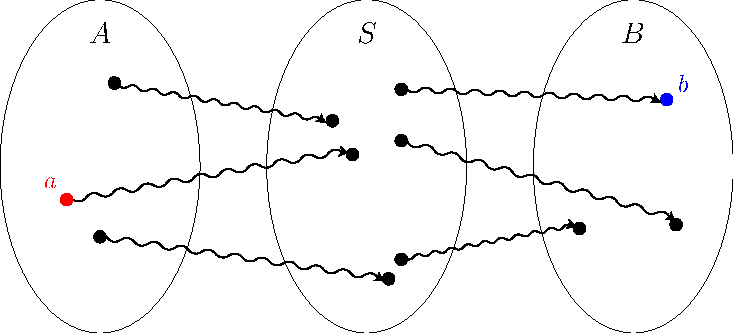
\includegraphics[width=0.5\linewidth]{greedy/graph-ab-separator.pdf}
    \caption{Example of an $(a,b)$-separator}
    \label{fig:graph-ab-separator}
\end{figure}

\begin{lemma} \label{lem:chordal-implies-separation}
    Given a chordal graph $G=(V,E)$ and two non-adjacent vertices $a,b \in V$ such that $(a,b) \not\in V$, any minimal $(a,b)$-separator induces a clique.
\end{lemma}

\begin{proof}
    By contradiction.

    Let $S$ be a minimal $(a,b)$-separator. Let $A,B$ be the two connected components separated by $S$, where $a \in A$ and $b \in B$. Suppose, for contradiction, that $S$ does not induce a clique, so there exists $u,v \in S$ such that $\{u,v\} \not\in E$. Since $S$ is minimal, there are edges from $u$ and $v$ to the subgraphs induced by $A$ and $B$. Otherwise, $S-\{u,v\}$ would have been a smaller $(a,b)$-separator.

    Let $p_a$ be the shortest path from $u$ to $v$, passing through vertices in $A$. Similarly, let $p_b$ be the shortest path from $v$ to $u$, passing through vertices in $B$. $p_a$ and $p_b$ each has path length of at least 2 because $u,v$ are not adjacent. It follows that the union of the two paths $p_a$ and $p_b$ is a cycle $u \to a_1 \leadsto a_k \to v \to b_1 \leadsto b_k \to u$ of length at least 4. Since $G$ is chordal, this cycle must contain a chord. But since this is the shortest cycle, there is no edge from $u,v$ to vertices in $A,B$ (otherwise, we can form a shorter cycle using this edge). There is no edge from vertices in $A$ to vertices in $B$ because the subgraphs they induce are disjoint. So, the chord must be between $u$ and $v$. However, this contradicts the assumption that $\{u,v\}\not\in E$.

    Hence, for every $u,v \in E$, $\{u,v\} \in E$.

    \begin{center}
        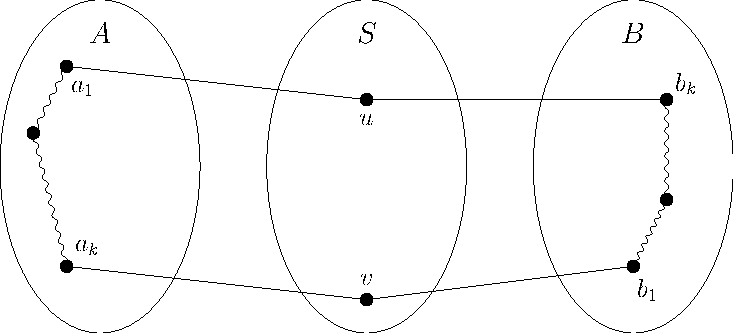
\includegraphics[width=0.5\linewidth]{greedy/graph-ab-sep-shortest-cycle.pdf}
    \end{center}
\end{proof}

\begin{lemma}[Dirac 1961] \label{lem:separation-implies-peo}
    Given a graph $G=(V,E)$, if all for all $a,b\in V$, the minimal $(a,b)$-separator induces a clique, then $G$ has a perfect elimination ordering.
\end{lemma}

\begin{proof}
    By induction on the number of vertices in $G$.

    \textbf{Base case}: When $n=1$, the lemma trivially holds.

    \textbf{Inductive step}: Let $n \in \N$. Assume that the lemma holds for all $k < n$.

    If $G$ is a complete graph, the whole graph is a clique, and we are done since every ordering is a perfect elimination ordering.

    Otherwise, there exists $a,b \in V$ such that $\{a,b\} \not\in E$. Let $S$ be a minimal $(a,b)$-separator in $G$. $S$ separates $V$ into disjoint subsets $A,S,B$. By assumption, $S$ induces a clique. Since the size of $A$ is strictly smaller than $V$, by induction hypothesis, we know that $A$ has a perfect elimination ordering. This implies that there exists $u \in A$ such that $\{u\} \cup N(u)$ induces a clique on the subgraph induced by $A$.

    Since $S$ separates $A$ and $B$, there is no edge going directly from vertices in $A$ to vertices in $B$. There is an edge connecting every pair of vertices in $S$, so if there are edges going between $u$ and vertices in $S$, the resulting subgraph is also a clique. Hence, $\{u\} \cup N(u)$ also induces a clique in $G$ because $S$ induces a clique.

    Consider the graph $G'$ obtained by removing vertex $u$ from $G$. $|V-\{u\}| < |V| = n$. By induction hypothesis, $G'$ has a perfect elimination ordering. Suppose the ordering is $(v_1,\ldots,v_{n-1})$. We can let $v_n = u$. By adding $v_n$ to the ordering, we get a new valid perfect elimination ordering because $v_{n}$ and its neighbors induces a clique in $G$.
    
    By induction, the lemma holds for graph of any size.
\end{proof}

\begin{figure}[htbp]
    \centering
    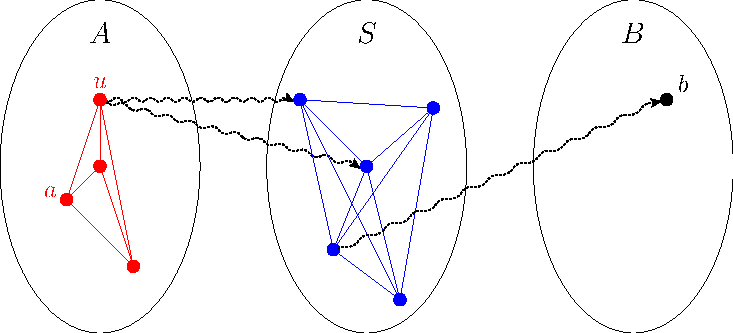
\includegraphics[width=0.5\linewidth]{greedy/graph-clique-separation.pdf}
    \caption{Proof idea for Lemma \ref{lem:separation-implies-peo}}
    \label{fig:graph-clique-separation}
\end{figure}

\begin{theorem}[Fulkerson and Gross 1965]
    A graph is a chordal graph if and only if it has a perfect elimination order.
\end{theorem}

\begin{proof}
    We will prove the theorem by proving the chain of implications that
    $$
    \text{(1) P.E.O.} \Rightarrow \text{(2) chordal graph}\Rightarrow \text{(3) minimal separator induces a clique} \Rightarrow \text{(1) P.E.O.}
    $$
    (1) $\Rightarrow$ (2): Let $C$ be a cycle of length at least 4 in $G$. Assume $G$ has a perfect elimination ordering. Then, take the perfect elimination ordering, and remove vertices by the ordering until we reach a vertex $c$ on the cycle $C$. Once we remove $c$, $N(c)$ induces a clique by definition of perfect elimination ordering. Therefore, there exists an edge between every two vertices in $C-\{c\}$. In other words, $C$ contains chords. Hence, $G$ is a chordal graph.

    (2) $\Rightarrow$ (3): By Lemma \ref{lem:chordal-implies-separation}.

    (3) $\Rightarrow$ (1): By Lemma \ref{lem:separation-implies-peo}.
\end{proof}

Tarjan and Yannakakis designed a linear-time algorithm called the maximum cardinality search for computing the perfect elimination ordering given a chordal graph \cite{Tarjan-Chordal-Graph}.

\begin{codebox}
    \Procname{$\proc{Compute-PEO}(G)$}
    \li \For all $v \in V$ \Do
        \li $\attrib{v}{label} = 0$
        \li $\sigma(v) = -1$ 
    \End
    \li \For $i=|V|$ \Downto 1 \Do
        \li $u = \mathrm{argmax}_{v \in V} \{ \attrib{v}{label} \mid \sigma(v) = -1 \}$ \quad \Comment{unvisited vertex with largest label}
        \li $\sigma(u) = i$ \quad \Comment{assign an order}
        \li \For neighbor $w$ of $v$ \Do
            \li \If $\sigma(w) \isequal -1$ \Then
                \li $\attrib{w}{label} = \attrib{w}{label} + 1$
            \End
        \End
    \End
    \li \Return $\sigma$
\end{codebox}

The algorithm starts by initializing the labels and numbers for each vertex. Then, it iteratively select unnumbered vertex with largest label to assign an order. With an naive implementation, Line 5 of the algorithm takes $O(|V|)$ time. However, this can be improved by using a disjoint set data structure. Let $S_i$ be the sets of unnumbered vertices with label $i$ for $0 \leq i \leq |E|-1$. Each $S_j$ is implemented using a linked list, and $[S_0,S_1,\ldots S_{i} ]$ is a direct access array indexed by $i$. Every time we increment the label of $w$, we move $w$ from $S_{i}$ to $S_{i+1}$ where in this case, $i$ is the $\attrib{w}{label}$. It is clear that this improved implementation runs in $O(|V|+|E|)$ time.

Finally, as promised, we will show an algorithm that solves the maximum independent set problem on an interval (chordal) graph.

\begin{codebox}
    \Procname{$\proc{MIS}(G)$}
    \li $\sigma = \proc{Compute-PEO}(G)$
    \li $I = \emptyset$
    \li \For $i = 1$ \To $|V|$ \Do
        \li $v = \sigma^{-1}(i)$
        \li $N = \{v \in N(v) \mid \sigma^{-1}(v) < i \}$
        \li \If $N \cap I \isequal \emptyset$ \Then
            \li $I = I \cup \{v\}$
        \End
    \End
    \li \Return $I$
\end{codebox}

The proofs in this section are based on the papers \textit{Incidence matrices and interval graphs} by Fulkerson and Gross \cite{Fulkerson1965-Chordal-Graph}, and \textit{On rigid circuit graphs} by Dirac \cite{Dirac1961-Rigid-Circuit-Graph}. The presentation of the proofs is loosely based on \textit{Advanced Topics in Graph Algorithms} by Ron Shamir \cite{shamir}.

\section{Minimum Spanning Tree}

A tree $(V,T)$ is a connected graph with no cycles (connected acyclic graph). Every node is reachable from every other node in exactly one way. If $(V,T)$ is connected, then $(V,T)$ is acyclic if and only if $|T| = |V|-1$.

\begin{definition}[Spanning Forest and Spanning Tree] \index{spanning forest} \index{spanning tree}
    Let $G = (V,E)$ be an undirected graph. A spanning forest of $G = (V,E)$ is an acyclic graph $(V,F)$ with $F \subseteq E$. It is a set of tree on disjoint sets of vertices.

    A spanning tree of $G$ is a connected spanning forest of $G$. It contains $|V| - 1$ edges.
\end{definition}

Kruskal's algorithm for MST proceeds by interatively merging subtrees of the input graph by picking the minimum weighted edge between the two subtrees. Prim's algorithm proceeds by starting from a single vertex and iteratively growing a tree from the vertex, again, by picking the minimum weighted edge as we expand the growing frontier of the current subtree.

\subsection{Kruskal's Algorithm} \index{Kruskal's algorithm}

\begin{codebox}
    \Procname{$\proc{Kruskal}(V,w)$}
    \li $A =  \emptyset$
    \li $Q = \proc{Priority-Queue}(\text{all edges $e$ where priority is $w(e)$})$
    \li \For $v \in V$ \Do
        \li $\proc{Make-Set}(v)$
        \End
    \li \While $|A| < n-1$ \Do 
        \li $\{u,v\} = \proc{Extract-Min}(Q)$ 
        \li $u' = \proc{Find-Set}(u)$
        \li $v' = \proc{Find-Set}(v)$
        \li \Comment{if $u$ and $v$ are in different components of $(V,A)$}
        \li \If $u' \neq v'$  \Then
            \li add $\{u,v\}$ to $A$ 
            \li $\proc{Link}(u',v')$
        \End
    \End
    \li \Return $(V,A)$ 
\end{codebox}

The optimality of Kruskal's algorithm can be proved using an exchange argument similar to the one that we used for the interval selection (job scheduling) problem.

\begin{theorem}[Correctness of Kruskal's Algorithm]
    If $G=(V,E)$ is a undirected connected graph with weight function $w:\,E \to \R$, when we run $\proc{Kruskal}$ on $G$, the algorithm returns a minimum spanning tree $(V,A)$.
\end{theorem}

\begin{proof}
    Let $A_i$ be the set of edges in $A$ after the $i$th iteration of the outer loop at Line 5. We will prove by induction the claim that for all $i \in \{0,\ldots,n-1\}$, there exists a set $T_i \subseteq \{e_{i+1},\ldots,e_n\}$ ordered by the weight of its elements, such that $A_i \cup T_i \subseteq A_{opt} \subseteq A_i \cup \{e_{i+1},\ldots,e_n\}$ where $A_{opt}$ is an optimal solution.

    \textbf{Base case}: When $i = 0$, $A_0 = \emptyset$. Since the graph is connected, there must exists a minimum spanning tree $A_{opt}$ and $A_0 \subseteq A_{opt} \subseteq A_0 \cup \{e_{i+1},\ldots,e_n\}$.

    \textbf{Inductive step}: Let $i \in \N$ be arbitrary. Suppose that the claim holds for $i$. This means $A_i \subseteq A_{opt} \subseteq A_i \cup \{e_{i+1},\ldots, e_n\}$. Let $e_{i+1} = \{u,v\}$ be the edge with $(i+1)$th smallest weight. Consider the following cases:

    (1) Adding $e_{i+1} = \{u,v\}$ forms a cycle. In this case, $e_{i+1}$ is not added to $A$ and $A_{i+1} = A_{i} \subseteq A_{opt} \subseteq A_i \cup \{e_{i+2},\ldots, e_n\}$.

    (2) Adding $e_{i+1} = \{u,v\}$ does not form a cycle and $e_{i+1} \in A_{opt}$. In this case, $e_{i+1}$ is added to $A$. $A_{i+1} = A_i \cup \{e_{i+1}\}$. But since $e_{i+1}$ is already in $A_{opt}$, $A_{i+1} = A_i \cup \{e_{i+1}\} \subseteq A_{opt} \cup \{e_{i+1}\} = A_{opt} \subseteq A_i \cup \{e_{i+2},\ldots,e_n\}$.

    (3) Adding $e_{i+1} = \{u,v\}$ does not form a cycle and $e_{i+1} \not\in A_{opt}$. $e_{i+1}$ is added to $A$. Since $A_{opt}$ is a spanning tree, it covers every vertices in $V$ so adding $e_{i+1}$ to $A_{opt}$ forms a cycle between $u$ and $v$. This implies that there exists an edge $e_j \in A_{opt} - A_{i+1}$ on the cycle since $A_{i+1}$ is acyclic. Removing $e_j$ from $A_{opt} \cup e_{i+1}$ breaks the cycle, and $A_{opt}' = A_{opt} - \{e_j\} \cup \{e_{i+1}\}$ is a spanning tree. Since $A_{opt} \subseteq \{e_{i+1},\ldots,e_n\}$ by inductive hypothesis, and $e_{i+1} \not\in A_{opt}$, we have $j > i+1$. Because $\{e_{i+1},\ldots,e_n\}$ is sorted in nondecreasing order by edge weight, we can conclude that $w(e_{i+1}) \leq e_j$. It follows that $w(A_{opt}') \leq w(A_{opt})$. Since $A_{opt}$ is already optimal, $w(A_{opt}') = w(A_{opt})$ and thus $A_{opt}'$ is also optimal. Furthermore, $A_{opt}' \subseteq A_{i+1} \cup \{e_{i+2},\ldots,e_n\}$.

    By induction, the claim holds for all $\{0,\ldots,n-1\}$. It follows that when the algorithm terminates after the final iteration, $A_{n} \subseteq A_{opt} \subseteq A_n \cup \emptyset = A_n$, so $A_n = A_{opt}$.
\end{proof}

In fact, this proof also shows the correctness of Prim's algorithm.

\subsection{Prim's Algorithm} \index{Prim's algorithm}

\begin{codebox}
    \Procname{$\proc{Prim}(V,r)$}
    \li \For $v \in V - \{r\}$ \Do
        \li $\attrib{v}{priority} = \infty$
        \li $\attrib{v}{parent} = \const{nil}$ \End
    \li $Q = \proc{Priority-Queue}(V-\{r\})$
    \li $u = r$ 
    \li \While $Q \neq \emptyset$ \Do
        \li \For neighbor $v$ of $u$ \Do
            \li \If $v \in Q$ \textbf{and} $w(\{u,v\}) < \attrib{v}{priority}$ \Then
                \li $\attrib{v}{priority} = w(\{u,v\})$
                \li $\proc{Decreae-Priority}(Q,v,\, \id{priority}=w(\{u,v\}))$ 
                \li $\attrib{v}{parent} = u$ \End
            \End
        \li $u = \proc{Extract-Min}(Q)$
        \li add $\{u,\attrib{u}{parent}\}$ to $A$
        \End
    \li \Return $(V,A)$ 
\end{codebox}

\section{Single-Source Shortest Path}

Given a weighted directed graph $G=(V,E)$ with a weight function $w:\; E \to \R$, we define the weight of a path $p = v_0,v_1,\ldots,v_k$ to be the sum of all edges on that path
$$
w(p) = \sum_{i=1}^k w(v_{i-1},v_i)
$$
Additionally, if there is a path from $u$ to $v$ in a graph $G$, let $\delta(u,v)$ denote the minimum weight of any of such path. Otherwise, define $\delta(u,v) = \infty$, meaning that $v$ is not reachable from $u$. 

A path $p$ from $u$ to $v$ is a shortest path if $w(p) = \delta(u,v)$.

\subsection{Dijkstra's Algorithm} \index{Dijkstra's algorithm}

The idea of \textit{\textbf{Dijkstra's algorithm}} is to construct a set of vertices $V'$ whose shortest path from $s$ has been determined. Each vertex $v \in V' - \{s\}$ has its predecessor $\attrib{v}{\id{parent}}$ on this path and $v.d$ is the weight of this path. One important limitation of Dijkstra's algorithm is that the graph \textbf{does not contain any edge with negative weight}.

Line 10-13 of the algorithm is known as ``edge relaxation''. Similar to Prim and Kruskal's algorithm, Dijkstra's algorithm is a greedy algorithm.  It orders the nodes based on their distances (or more precisely, the current estimate of distances at a given stage of the algorithm, $d$) from $s$. At each step of the algorithm (the outer while loop), the algorithm looks at the node $u$ with the smallest $d$ and perform edge relaxation between $u$ and its neighbors.

\begin{codebox}
    \Procname{$\proc{Dijkstra}(G,s)$}
    \li \For $v \in V - \{s\}$ \Do
        \li $v.d = \infty$
        \li $\attrib{v}{parent} = \const{nil}$
        \End
    \li $s.d = 0$
    \li $\attrib{s}{parent} = s$
    \li $Q = \proc{Priority-Queue}(V,\, \id{key}=d)$
    \li \While $Q \neq \emptyset$ \Do
        \li $u = \proc{Extract-Min}(Q)$
        \li \For neighbor $v$ of $u$ \Do
            \li \If $v \in Q$ \textbf{and} $v.d > u.d + w(\{u,v\})$ \Then
                \li $v.d = u.d + w(\{u,v\})$
                \li $\proc{Decrease-Priority}(Q,v,\, \id{priority}=u.d+w(\{u,v\}))$
                \li $\attrib{v}{parent} = u$   
\end{codebox}

\chapter{Huffman Encoding}

\chapter{Generalizing and Formalizing Greedy}
\section{Priority Model}

For a given problem, we assume that the input items belong to some set $\mathcal{J}$. For any execution of the algorithm, the input is a finite subset $\mathcal{I} \subset \mathcal{J}$.

Let $f:\,\mathcal{J} \to \R$ be a function. We do not place restriction on the complexity or computability of such function. For an input set $\mathcal{I} = \{I_1,\ldots,I_n\}$, the function induces a total ordering $\preceq$ on $\mathcal{I}$, breaking ties using certain rules (for example, by input ID).

For a fixed order priority algorithm, $f$ and $\preceq$ are set initially before the algorithm observes the input set. For adaptive order, the algorithm computes $f$ and $\preceq$ dynamically. More formally, there is a different function $f_i$ and ordering $\preceq_i$ associated with each iteration $i$ where $f_i$ and $\preceq$ depends on the items $\{I_1,\ldots,I_{j}\}$ considered in prior iterations $j < i$. 

Let us first consider fixed order algorithm under this priority model. In each iteration $k$ for $1 \leq k \leq n$, the algorithm observes input element $I_k \in \mathcal{I}$ and based on this input and all previous inputs and decisions, the algorithm makes an irrevocable decision $D_k$ about this input item (this typically involves whether to include or discard the current item).

This model gives us the following template for fixed order priority algorithms

\begin{codebox}
    \li $\mathcal{J} =$ set of all possible inputs
    \li $\preceq\,\, = $ a total ordering on $\mathcal{J}$ (typically induced by a function $f$)
    \li $\mathcal{I} \subset \mathcal{J} = $ actual input to the algorithm
    \li $S = \emptyset$ \RComment{items already examined by the algorithm}
    \li $i = 0$
    \li \While $\mathcal{I} - S \neq \emptyset$ \Do
        \li $i = i + 1$
        \li $\mathcal{I} = \mathcal{I} - S$
        \li $I_i = \min_{\preceq} \{ I \in \mathcal{I} \}$ \RComment{select min element based on the ordering $\preceq$}
        \li make an irrevocable decision $D_i$ concerning $I_i$ 
        \li $S = S \cup \{I_i\}$
    \End      
\end{codebox}

This template can be modified to allow the algorithm to determine the total ordering dynamically based on the elements it has observed so far.

\begin{codebox}
    \li $\mathcal{J} =$ set of all possible inputs
    \li $\mathcal{I} \subset \mathcal{J} = $ actual input to the algorithm
    \li $S = \emptyset$ \RComment{items already examined by the algorithm}
    \li $i = 0$
    \li \While $\mathcal{I} - S \neq \emptyset$ \Do
        \li $i = i + 1$
        \li $\preceq_i\,\, = $ a total ordering on $\mathcal{J}$ (typically induced by a function $f_i$)
        \li $\mathcal{I} = \mathcal{I} - S$
        \li $I_i = \min_{\preceq_i} \{ I \in \mathcal{I} \}$ \RComment{select min element based on the ordering $\preceq_i$}
        \li make an irrevocable decision $D_i$ concerning $I_i$ 
        \li $S = S \cup \{I_i\}$
        \li $\mathcal{J} = \mathcal{J} - \{I \in \mathcal{I} \mid I \preceq_i I_i \}$
    \End      
\end{codebox}

For greedy algorithm, the algorithm does not have knowledge of the input other than the elements it has observed so far. Sometimes, we allow the algorithm to have some easily computed global information such as the size of the input. The input is said to be chosen by an adversary.

This generalization applies to a broader category of algorithms known as priority-based algorithms. Informally, greedy algorithms always assume that the current iteration could be the last one and the current item being considered might as well be the last item. Hence, an optimal decision is immediate when the algorithm finishes. A more general priority algorithm that are not necessarily greedy does not have such restriction

This formalization was first given by Allan Borodin \textit{et al.} in \textit{(Incremental) Priority Algorithms} (Thirteen Annual ACM-SIAM Symposium on Discrete Algorithms, January 2002) \cite{borodin-priority}.

\section{Global Optimality of Greedy Algorithms}

(From Allan Borodin's notes)

Most greedy algorithms are not opitmal. The method we use to show that a greedy algorithm is optimal (when it is) known as the exchange argument often proceeds as follws. At each stage $i$, we define our partial solution to be promising if it can be extended to an optimal solution by using elements that haven't been considered yet by the algorithm; that is, a partial solution is promising after stage $i$ if there exists an optimal solution that is consistent with all the decisions made through stage $i$ by our partial solution. We prove the algorithm is optimal by fixing the input problem, and proving by induction on $i \geq 0$ that after stage $i$ is performed, the partial solution obtained is promising. The base case of $i=0$ is usually completely trivial: the partial solution after stage O is what we start with, which is usually the empty partial solution, which of course can be extended to an optimal solution. The hard part is always the induction step, which we prove as follmvs. Say that stage $i+1$ occurs, and that the partial solution after stage $i$ is $S_i$ and that the partial solution after stage $i+1$ is $S_{i+1}$, and we know that there is an optimal solution $S_{opt}$ that extends $S_i$; we want to prove that there is an optimal solution $S_{opt}'$ that extends $S_{i+1}$. $S_{i+1}$ extends $S_i$ by taking only one decision; if $S_{opt}$ makes the same decision, then it also extends $S_{i+1}$, and wve can just let $S_{opt}' = S_{op}$ and we are done. The hard part of the induction step is if $S_{opt}$ does not extend $S_{i+1}$, In this case, we have to show either that $S_{opt}$ could not have been optimal (implying that this case cannot happen), or we show how to change some parts of $S_{opt}$ to create a solution $S_{opt}'$ such that

\begin{itemize}
    \item $S_{opt}'$ extends $S_{i+1}$ and
    \item $S_{opt}'$ has value (cost, profit, etc.) at least as good as $S_{opt}$, so the fact that $S_{opt}$ is optimal implies that $S_{opt}'$ is optimal.
\end{itemize}

For most greedy algorithms, when it ends, it has constructed a solution that cannot be extended to any solution other than itself. Therefore, if we have proven the above, we know that the solution constructed by the greedy algorithm must be optimal.

\part{Dynamic Programming}

\chapter{Weighted Interval Selection}
\section{Dynamic Programming} \index{dynamic programming} \index{memoization}

\textit{\textbf{Dynamic programming}} (DP) is a method for solving complex problem by breaking it down to a collection of simpler subproblems, solving each of those subproblems, and storing their solutions. The next time the same subproblem occurs, instead of recomputing the solution, the algorithm can just use the previously computed solution. Each subproblem is indexed in some way to facilitate the lookup. The technique of storing solutions to subproblems is called \textbf{memoization}.

Let's consider the weighted interval selection problem.

\section{Weighted Interval Selection}

The objective of the weighted interval selection problem is to find a non-intersecting set of intervals so that the sum of the weights of intervals in the set is minimized. More formally, given a set of jobs/activities $\{a_1,\ldots,a_n\}$ with start time $s_i$ and finish time $f_i$ and weight $w_i$, we want to find a set $S$ of mutually compatible jobs with highest total weight $\sum_{i \in S} w_i$ 

Note that when $w_i = 1$ for all $i = \{1,\ldots,n\}$, the weighted interval selection problem is the same as simple interval scheduling.

We first consider greedy algorithms. Possible choices for the greedy choice include: weights, interval length, etc. Unfortunately, all the possible ways of ordering the input items will not only fail to give an optimal solution, but can in fact produce arbitrarily bad solutions for some instances. With a generalized greedy approach, it can be proved that no greedy algorithm can produce a good solution. With certain modifications/extensions to greedy, the algorithm can produce a good approximation (by allowing revocable decisions) and even optimal solution (using local ratio/primal dual algorithms with a reverse delete phase).

\section{Computing the Optimal Weight}
\subsection{The Dynamic Programming Approach}

Assume that the jobs (intervals) have been sorted by non-decreasing finish time. Then, in an optimal solution $O$, either the last interval $I_n$ was selected, or it was not. If not, then we must be using an optimal solution for the first $n-1$ intervals. If $a_n$ is in $O$, then no interval in $O$ can end after the starting time of $a_n$.

Let us now make this intuition more concrete. Given that the jobs are sorted by non-decreasing finish time, let $\id{pred}(i)$ be the largest index $j < i$ such that $f_j < s_j$. This means that jobs $a_1,\ldots,a_j$ are compatible with $a_i$, but $a_{i+1},\ldots,a_{j-1}$ are not compatible.

Let $O$ be an optimal solution. For each job $a_i$, there are two possibilities:
\begin{itemize}
    \item Job $a_i \in O$: This implies that $\{\id{pred}[i]+1,\ldots,a_{i-1}\}$ are all incompatible with $a_i$. So, we must select jobs from $\{a_1,\ldots,\id{pred}[i]\}$.
    
    \begin{center}
        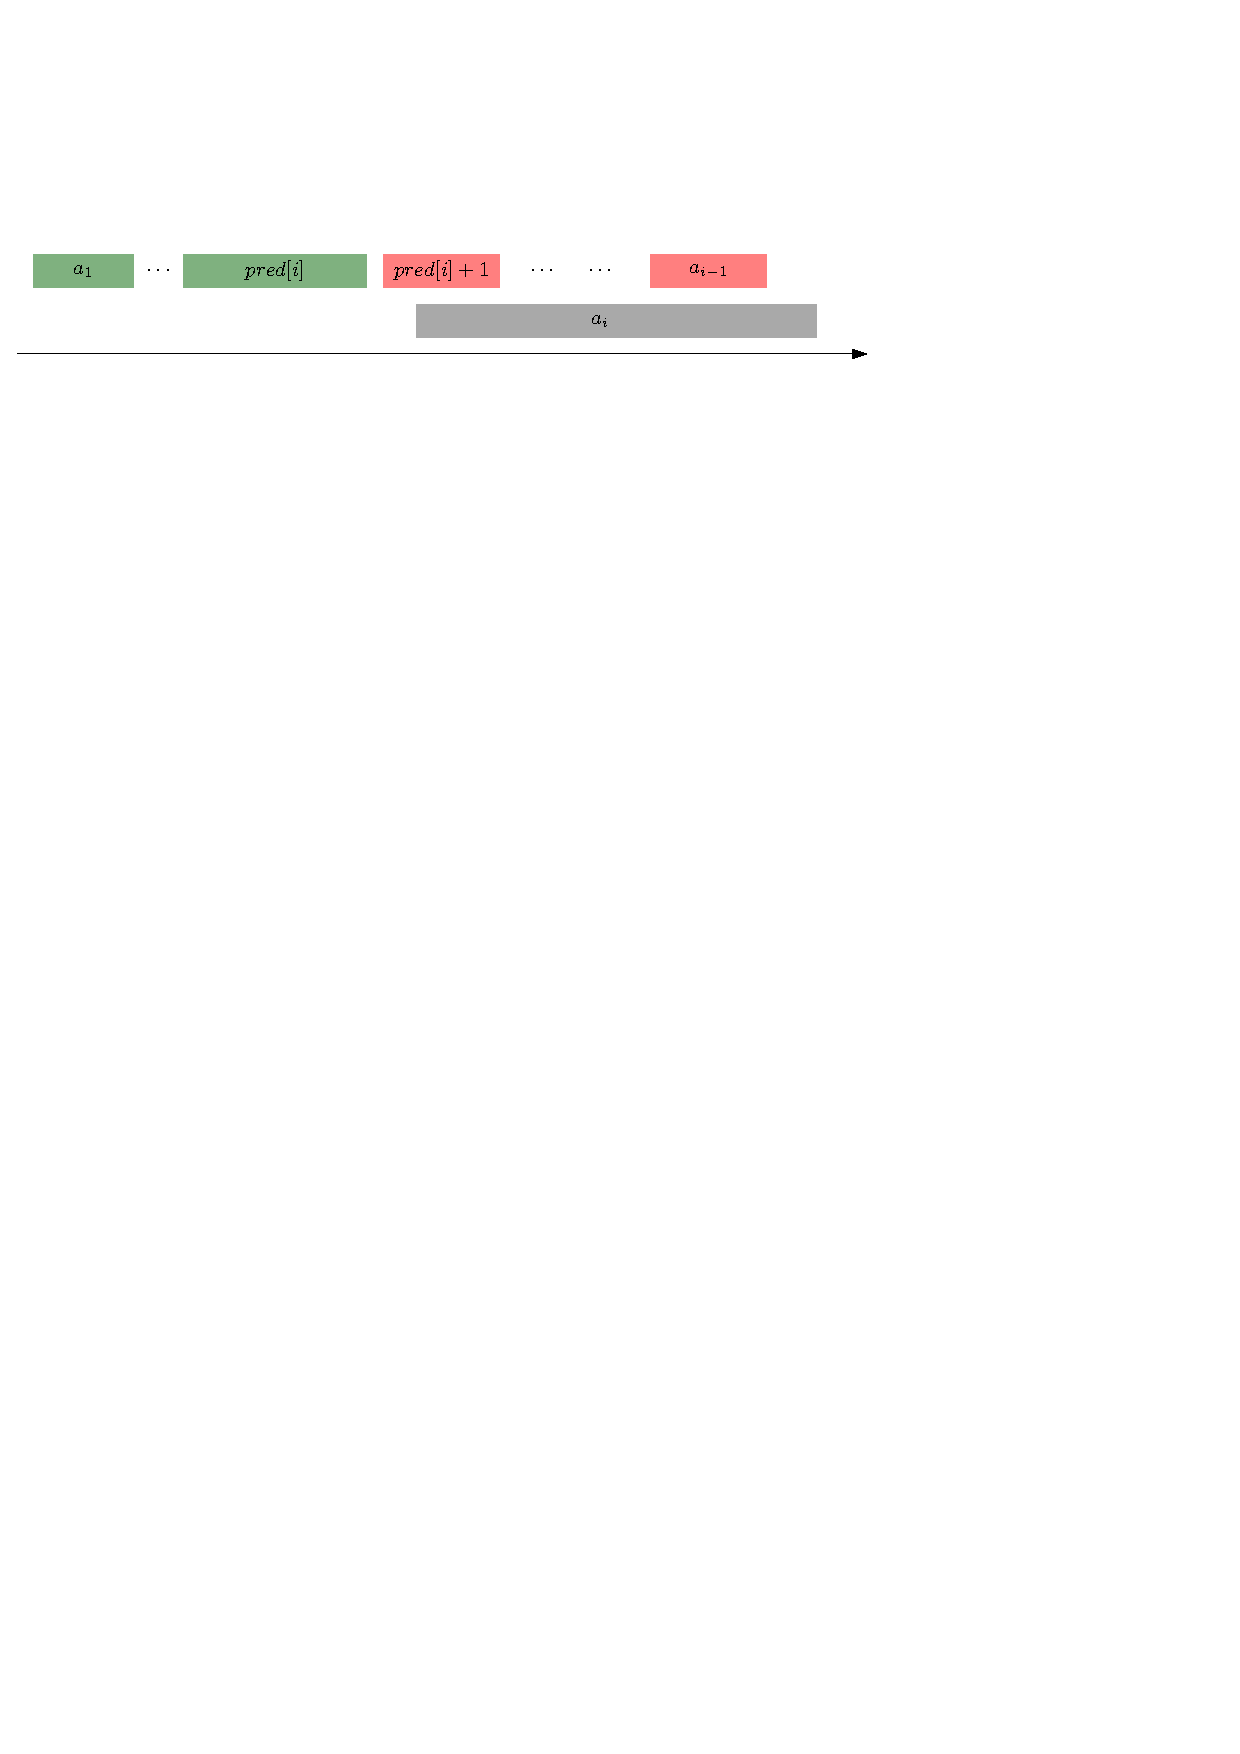
\includegraphics[width=0.8\linewidth]{dp/wisp/wisp-opt-case1.pdf}
    \end{center}

    \item Job $a_i \not\in O$: This implies that we must select jobs from $\{a_1,\ldots,a_{i-1}\}$. 
    
    \begin{center}
        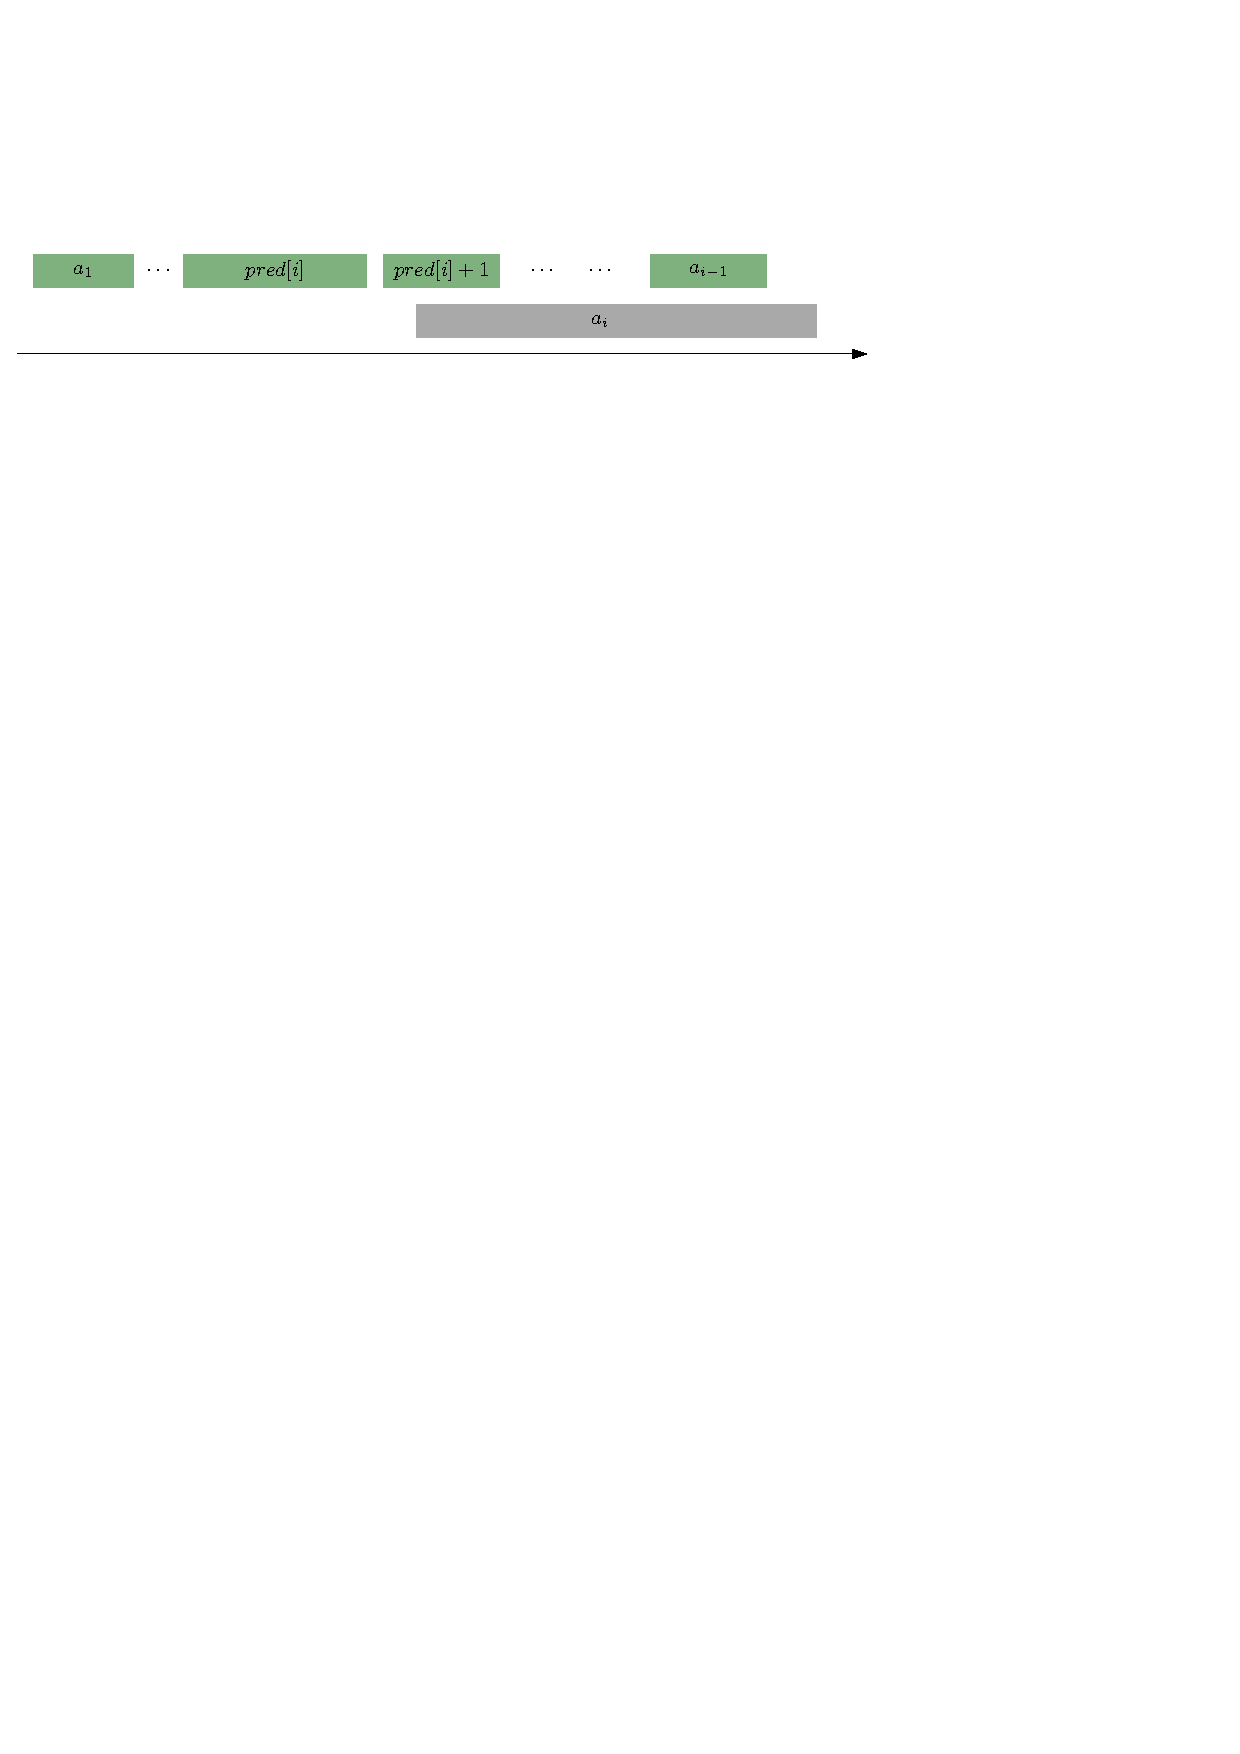
\includegraphics[width=0.8\linewidth]{dp/wisp/wisp-opt-case2.pdf}
    \end{center}
\end{itemize}

Let define $V:\; \{a_1,\ldots,a_n\} \to \R$ be defined such that
$$
V(i) = \text{max total weight of compatible jobs from $\{a_1,\ldots,a_i\}$}
$$
More formally, $V$ can be expressed as this recurrence
$$
V(i) = \begin{cases}
    0 & i = 0 \\
    \max \{V(i-1),w_i+V(\id{pred}[i]) \} & i > 0
\end{cases}
$$
\begin{lemma}
    The two definitions of $V$ are equivalent.
\end{lemma}
\begin{proof}
    By induction.
\end{proof}
\index{semantic array} \index{Bellman equation}
Sometimes, the first definition of $V$ in English is represented as an array indexed by $i$ and referred to as a \textit{\textbf{semantic array}}. The second equation of $V$ is called the \textit{\textbf{Bellman equation}}.

This recurrence gives us a clear recursive solution for the weighted interval selection problem.

Consider the time complexity of the naive recursive implementation. $\id{pred}[i]$ can be computed using binary search in $O(\log n)$ time, and for all of the $n$ values to be considered, this takes $O(n \log n)$ time. However, the time spent on computing $\id{pred}$ turns out to be rather insignificant compared to the running time of the main algorithm.
$$
T(n) = T(n-1) + T(\id{pred}[n]) \leq T(n-1) + T(n-2) \in \Theta(\varphi^n)
$$
where $\varphi \approx 1.618$ is the golden ratio. This is a Fibonacci recurrence.

This is clearly bad. Some solutions are being computed many times unnecessarily. Recall that one of the most important component of dynamic programming is memoization. In many cases, without memoization, dynamic programming simply becomes divide and conquer, or even worse, recurrence that runs in exponential time like this one. Memoization allows us to remember the results that we have already computed and reuse them if needed.

\subsection{Top-Down DP}
In our first dynamic programming implementation, we will store the previously computed values in the array $M$ indexed by the index of each interval.

Assume that prior to calling $\proc{Compute-Opt-DP}(n)$, the intervals are sorted in nondecreasing order based on finish time, $\id{pred}$ has been precomputed in $O(n\log n)$ time, and $M$ is a global array of size $n$ with every entry set to 0 initially.

\begin{codebox}
    \Procname{$\proc{Compute-Opt-DP}(j)$}
    \li \If $M[j] \isequal \const{nil}$ \Then 
        \li $M[j] = \max\{\proc{Compute-Opt-DP}(j-1),\; w_j + \proc{Compute-Opt-DP}(\index{pred}[j]) \}$
    \End
    \li \Return $M[j]$
\end{codebox}

For each $i = \{1,\ldots,n\}$, there is only one call to $\proc{Compute-Opt-DP}(i)$ because previously computed values are stored in the array $M$. Therefore, there are at most $O(n)$ calls to the recursive procedure. Sorting by finish time and computing $\id{pred}$ takes $O(n \log n)$ time, so the overall time complexity of this implementation is $O(n \log n)$. Much better than our original exponential implementation!

\subsection{Bottom-Up DP}

The bottom-up approach differs from the top-down approach in that values of $M$ are precomputed. Instead of using recursive call and checking if $M[i] \isequal \const{nil}$, we can simply reference to indices of the array where previously computed values are stored. Assume the same preconditions are met prior to calling \proc{Compute-Opt-DP-Botton-Up}.

\begin{codebox}
    \Procname{$\proc{Compute-Opt-DP-Botton-Up}()$}
    \li \For $j = 1$ to $n$ \Do
        \li $M[j] = \max\{M[j-1],\, w_j + M[\id{pred}[j]] \}$
    \End
    \li \Return $M[n]$ 
\end{codebox}

It can be shown using a simple loop invariant and induction that at the beginning of the $i$th iteration, $M[j]$ is already computed for all $j < i$ and thus we will not get a null pointer error.

This approach has the same time complexity as the top-down approach.

\subsection{Comparison of Two Approaches}

Top-down may be preferred when not all sub-solutions need to be computed on some inputs. This helps us save some time.

Bottom-up may be preferred when all sub-solutions will always need to be computed for all inputs. The bottom-up approach could be faster as it prevents unnecessary recursive calls which results in unnecessary random memory access. This is because even though recursive dynamic programming does not compute repeated results, there could still be redundant recursive calls, resulting in a large overhead.

\section{Computing the Optimal Solution}

In the previous section, we come up with a dynamic programming algorithm that computes the optimal weight of the solution set for the weighted interval selection problem. Now, we will extend that algorithm so that we get the actual solution set (subset of $S$ that maximizes weight). We only need a really simple modification from the original definition of $V$. Recall that $V$ is defined as
$$
V(i) = \begin{cases}
    0 & i = 0 \\
    \max \{V(i-1),w_i+V(\id{pred}[i]) \} & i > 0
\end{cases}
$$
Instead of calculating values, we want a subset of the input set.
$$
S(i) = \begin{cases}
    \emptyset & i = 0 \\
    S(i-1) & \text{if $V(i) = V(i-1)$} \\
    S(\id{pred[i]}) \cup \{ a_i \} & \text{otherwise}
\end{cases}
$$
We can either precompute $V$ and uses it directly in the implementation of $S$. Or alternatively, we can compute $V$ and $S$ simultaneously.

\chapter{Knapsack Problem}
\section{Knapsack} \index{knapsack problem}

In the knapsack problem, we are given a set of $n$ items $I_1,\ldots,I_n$ and a size bound $B$ where each item $I_j=(w_j,v_j)$ with $w_j$ being the weight of the item and $v_j$ the value of the item.

A subset of items $S$ is feasible if the sum of the weights of items in $S$ is at most $B$. The goal of the knapsack problem is to find a feasible set $S$ that maximizes the sum of the values of items in $S$.

\section{DP Algorithm for 0-1 Knapsack}

We define the semantic array
$$
V(i,b) = \text{max profit possible using the first $i$ items within weight $b$}
$$
with corresponding Bellman equation
$$
V(i,b) = \begin{cases}
    0 & \text{if $i=0$ or $b=0$} \\
    \max\{C,D\} & \text{if $w_i \leq b$}
\end{cases}
$$
where $C = V(i-1,b)$ and $D = V(i-1,b-w_i) + v_i$.

$C$ corresponds to the decision to not include the $i$th item in the knapsack, and $D$ correspond to the decision to include the $i$th item, in which case we deduce $w_i$ from the remaining weight of the knapsack and add $v_i$ to the total profit. Like all DP problems, we need to prove that the semantic array is equivalent to the Bellman equation.

\begin{codebox}
    \Procname{$\proc{Knapsack}(S,B)$}
    \li $n = \attrib{S}{length}$ 
    \li \For $b=0$ to $B$ \Do
        \li $M[0,b] = 0$
    \End
    \li \For $i=1$ to $n$ \Do
        \li \For $b = 0$ to $B$ \Do
            \li \If $S[i].w > b$ \Then
                \li $M[i,b] = M[i-1,b]$
            \li \Else
                \li $M[i,b] = \max\{M[i-1,b],\, S[i].v + M[i-1,b-1]\}$
            \End
        \End
    \End
    \li $M[n,B]$ 
\end{codebox}

The input to the algorithm: $S$ is the set of all items to be considered, and $B$ is the weight bound of the knapsack. This approach makes an important assumption that the weights are integer.

\index{pseudopolynomial}
This DP algorithm solving the 0-1 knapsack problem with $n$ items and weight bound $B$ runs in $\Theta(nB)$ time and uses $\Theta(nB)$ space. As we can see, the running of this algorithm is, unfortunately, not polynomial in the input size. It is \textbf{pseudo-polynomial}. It is polynomial in $\log B + \sum_{i=1}^n (\log v_i + \log w_i)$.

If $B$ is small (a polynomial in $n$), then the algorithm runs in polynomial time. No known exact algorithm runs in polynomial time. The 0-1 knapsack problem is NP-complete.

\section{A Different DP Algorithm}

Consider version of the knapsack problem with a different restriction that the values $v_i$ are integer and small ($V=\sum_{i=1}^n v_i \ll B$). In this case, it makes more sense to derive an algorithm in terms of $v$ instead of $B$.

The semantic array is defined as follows
$$
W(i,v) = \begin{cases}
    \substack{\text{minimum weight required to obtain at least} \\ \text{profit $v$ using a subset of $\{I_1,\ldots,I_i\}$}} & \text{if possible} \\
    \infty & \text{otherwise}
\end{cases}
$$
The goal is to compute $\max\{v \mid W(n,v) \leq B\}$.

The corresponding Bellman equation is
$$
W(i,v) = \begin{cases}
    \infty & \text{if $i=0$ and $v>0$} \\
    0 & \text{if $i\leq 0$ or $b\leq 0$} \\
    \max\{C,D\} & \text{otherwise}
\end{cases}
$$
where $C = W(i-1,v)$ and $D=W(i-1,v-v_i) + w_i$.

This algorithm is still pseudo-polynomial but the complexity is now $O(nV)$ where $V = v_1 + \cdots + v_n$. This is more efficient when $V \ll B$.

\section{FPTAS Approximation for Knapsack}

Because 0-1 knapsack is NP-complete, it is also of theoretical interest to find an efficient approximation algorithm. In the case of the knapsack problem, it is possible to find an algorithm that approximates the result within a specific degree on all possible inputs.

The idea behind the algorithm is as follows: The high order bits/digits of the value $v$ can be used to determine an approximate solution. The fewer high order bits we use, the faster the algorithm runs, but also the worse the approximation.

The goal is to scale the values $v$ using a parameter (rounding factor) $\epsilon$ so that a $(1+\epsilon)$ approximation is obtained with time complexity polynomial in $n$ and $1/\epsilon$.

More precisely, let $\tilde{v} = \lceil v_i/b \rceil b$. This ensures that the constraint that $v$ must be integer for the second algorithm is satisfied. By rounding the values, we get an approximation $\tilde{v}$ of $v$ that is divisible by $b$. This means we can divide all values of $v$ by $\epsilon$ and get an equivalent problem. Let $\hat{v} = \tilde{v}/b$. This allows us to reduce the size of $v$ so that it becomes smaller than $n$ (or at least bounded by a polynomial in $n$).

\begin{codebox}
    \Procname{$\proc{Knapsack-Approx}(\epsilon,S)$}
    \li $b = (\frac{\epsilon}{2n}) \cdot \max_i v_i$
    \li \For $i$ in $S$ \Do 
        \li $\tilde{v} = \lceil v_i/b \rceil b$
        \li $\hat{v} = \tilde{v}/b$
        \li $i.v = \hat{v}$
    \End
    \li $\proc{Knapsack-V}(S,\max_i\{v_i\})$ 
\end{codebox}
where $\proc{Knapsack-V}$ is the second DP algorithm discussed above.

\proc{Knapsack-Approx} is a \textbf{FPTAS} (fully polynomial time approximation scheme) algorithm for the 0-1 knapsack problem.

\begin{definition}[FPTAS and PTAS] \index{FPTAS} \index{PTAS}
    \hfill \\
    An \textbf{FPTAS} (Fully Polynomial Time Approximation Scheme) algorithm is one that is polynomial in the encoding of the input and $1/\epsilon$.

    A \textbf{PTAS} (Polynomial Time Approximation Scheme) algorithm is one that is polynomial to the encoding of the algorithm but can have any complexity in terms of $1/\epsilon$ ($1/\epsilon$ term may not be polynomial).
\end{definition}

\chapter{Graph Algorithms Using DP}
\section{Single-Source Shortest Path}

We have discussed single-source shortest path when we talked about greedy algorithms.

Previously, we have restricted our discussion to graphs without negative weights/cycles. In this chapter, we will talk about algorithms that can be used to general graphs (even one with negative cycles). 

Recall that we store the weight of the path from the source $s$ to each node $u$ at $u.d$. Consider a shortest path $p$ from $s$ to a vertex $v$. If there is a vertex $u$ immediately preceding $v$ on such path, then the path from $s$ to $u$ must also be a shortest path.

One caveat we must consider is that if there is a negative cycle in the graph, one can keep traversing through that negative cycle and yield a path with lower weight. If this happens, the algorithm can get stuck in a negative cycle and $d$ values may never converge. Hence, we need to put one additional constraint: only consider path within certain path length. Let $\delta_k(s,v)$ denote the shortest path from $s$ to $v$ using at most $k$ edges. Similarly, for a vertex $v$, let $v.d_k$ be the weight of the path from $s$ to $v$ using at most $k$ edges.

In addition, we will define some notations to aid our discussion. If $v$ is immediately reachable from $u$ via one edge, we write $u \to v$. If $v$ is reachable from $u$ via multiple edges, we write $u \leadsto v$.

\subsection{Bellman-Ford} \index{Bellman-Ford algorithm}

An obvious dynamic programming solution follows from this Bellman equation
$$
v.d_k = \begin{cases}
    0 & \text{if $k=0$ and $v=s$} \\
    \infty & \text{if $k=0$ and $v \neq s$} \\
    \min\{A,B\} & \text{otherwise}
\end{cases}
$$
where $A = v.d_{k-1}$ and $B = \min\{u.d_{k-1} + w(u,v) \mid (u,v) \in E \}$.
To prove the correctness of this equation, we can use induction on the length of the path $k$.

For a simple shortest path, there are at most $|V|-1$ edges. There will be $O((|V|-1)|V|) \in O(|V|^2)$ because we may need to update the $d$ field of all $|V|$ vertices. Each call takes $O(|E|)$ time in order to evaluate $B = \min\{u.d_{k-1} + w(u,v) \mid (u,v) \in E \}$. Therefore, the overall running time of the algorithm is in $O(|V|^2|E|)$.

The dynamic programming algorithm is a somewhat worse version of the Bellman-Ford algorithm, which runs in $O(|V|\cdot|E|)$ time with space complexity $O(|V| + |E|)$.

This rather unfortunate $O(|V|^2|E|)$ running time partly originates from the fact that we are updating the $d$ field of each $v$ for all $v \in |V|$. But if for every $v$, we are taking $O(|E|)$ time to examine all the edges to update $v.d$ anyway, we might as well just update all the $d$ fields whenever we run a pass through $E$. This gives us an algorithm with running time $O(|V|\cdot |E|)$. The $|V|$ comes from the $|V|-1$ iterations to optimize (``relax'') each edge on the simple shortest path of at most $|V|-1$ edges, and the $|E|$ comes from the pass through $E$ during each of the $|V|-1$ iterations to update the $d$ fields.

Using the following set of lemmas, we will show that it is safe to do so.

\begin{lemma}[Triangle Inequality] \index{triangle inequality (shortest path)}
    For any edge $(u,v) \in E$, we have $\delta(s,v) \leq \delta(s,u) + w(u,v)$.
\end{lemma}
\begin{proof}
    By contradiction.

    Suppose the claim does not hold. In particular, let $\delta(s,v) > \delta(s,u) + w(u,v)$. This implies that the shortest path from $s$ to $v$ has a higher weight than the path $s \leadsto u \to v$. But this contradicts the fact that $\delta(s,v)$ is the shortest path.
\end{proof}

\begin{lemma}[Upper-bound Property] \index{upper-bound property}
    We always have $v.d \geq \delta(s,v)$ for all verticies $v \in V$, and once $v.d$ is equal to $\delta(s,v)$, it never changes.
\end{lemma}
\begin{proof}
    By induction on the number of relaxations.

    Base case: $v.d \geq \delta(s,v)$ after initialization since $v.d = \infty$ for all $v \in V - \{s,v\}$, and for $s.d = 0 = \delta(s,s)$.

    Inductive step: Consider the relaxation of an arbitrary edge $(u,v)$. Assume that $x.d \geq \delta(s,x)$ for all $x \in V$ prior to relaxation. The relaxation of $(u,v)$ can only affect $v.d$. If $v.d$ is updated, then
    $$
    \begin{aligned}
        v.d &= u.d + w(u,v) \\
        &\geq \delta(s,u) + w(u,v) & \text{inductive hypothesis} \\
        &\geq \delta(s,v) & \text{triangle inequality}
    \end{aligned}
    $$
    The invariant is maintained after relaxing $(u,v)$.

    Once $v.d = \delta(s,v)$, $v.d$ cannot decrease because $v.d \geq \delta(s,v)$ always holds and relaxation cannot increase $v.d$.
\end{proof}

\begin{lemma}[No-path Property] \index{no-path property}
    If there is no path from $s$ to $v$, then we always have $v.d = \delta(s,v) = \infty$.
\end{lemma}
\begin{proof}
    Follows immediately from the upper-bound property.
\end{proof}

\begin{lemma}[Convergence Property] \index{convergence property}
    If $s \leadsto u \to v$ is a shortest path in $G$ for some $u,v \in V$, and if $u.d = \delta(s,u)$ at any time prior to relaxing edge $(u,v)$, then $v.d = \delta(s,v)$ at all times afterward.
\end{lemma}
\begin{proof}
    By upper bound property, once $u.d = \delta(s,u)$, it no longer changes. In particular, after relaxing $(u,v)$, we have
    $$
    \begin{aligned}
        v.d &\leq u.d + w(u,v) & \text{Lemma 24.13, CLRS} \\
        &= \delta(s,u) + w(u,v) \\
        &= \delta(s,v) & \text{Lemma 24.1, CLRS}
    \end{aligned}
    $$
    (Note that Lemma 24.1 was proved in the chapter covering Dijkstra's algorithm in my \href{https://github.com/gaojunxuan/data_struct_notes}{\color{ocre}notes on data structures}, CSC265 Notes)
    
    By the upper bound property, $v.d \geq \delta(s,v)$. It follows that $v.d = \delta(s,v)$.
\end{proof}

\begin{lemma}[Path-relaxation Property] \index{path-relaxation property} \index{path relaxation}
    If $p = v_0,v_1,\ldots,v_k$ is a shortest path from $s = v_0$ to $v_k$, and we relax the edges of $p$ in the order $(v_0,v_1),(v_1,v_2),\ldots,(v_{k-1},v_k)$, then $v_k.d = \delta(s,v_k)$. This property holds regardless of other relaxations that occur, including those intermixed with relaxations of edges in $p$.
\end{lemma}

\begin{proof}
    Proof by induction on the $i$th edge of $p$ that is relaxed.

    Base case: $i=0$. This is before any edge of $p$ have been relaxed. From initialization, $v_0.d=\delta(s,s)=0$. By upper bound property, $v_0.d$ does not change once it converges to $\delta(s,v_0)$ 
    
    Inductive step: Assume that $v_{i-1}.d = \delta(s,v_{i-1})$. We relax edge $(v_{i-1},v_i)$. By convergence property, after relaxation of this edge, $v_i.d = \delta(s,v_i)$, and by upper bound property, this equality is maintained thereafter.
\end{proof}

From the path-relaxation property, we can prove the correctness of Bellman-Ford on a graph without negative-weight cycles.

\begin{theorem}[Correctness of Bellman-Ford (without negative cycle)]
    Let \proc{Bellman-Ford} be run on a weighted directed graph $G=(V,E)$ without negative cycles, with source $s$ and weight function $w:\; E \to \R$. Then, the algorithm terminates and when it does, $v.d = \delta(s,v)$ for all vertices $v \in V$, from which we can construct a predecessor subgraph $G_\pi$ that is a shortest path tree.
\end{theorem}

\begin{proof}
    We first prove that at termination, $v.d = \delta(s,v)$ for all vertices $v \in V$. If $v$ is not reachable from $s$, the claim follows from the no-path property. If $v$ is reachable from $s$, then consider a shortest path $p = v_0,v_1,\ldots,v_k$ where $v_0=s$ and $v_k = v$. Because the shortest path is simple in a graph without negative cycle, so $k \leq |V|-1$. Each of the $|V|-1$ iterations of the outer loop of the algorithm relaxes all $|E|$ edges. Among the edges relaxed in the $i$th iteration in the $|V|-1$ total iterations, is $(v_{i-1},v_i)$. By path-relaxation property, $v.d = v_k.d = \delta(s,v_k) = \delta(s,v)$ even if other relaxation steps are intermixed within the sequence of relaxations of edges $(v_0,v_1),\ldots,(v_{k-1},v_k)$. Hence, the claim holds when $v$ is reachable from $s$.

    By the predecessor-subgraph property (Lemma 24.17, CLRS), $G_\pi$ is a shortest-path tree.

    Termination of the algorithm follows from the fact that the loop-counters of both loops are strictly increasing.
\end{proof}

Let us finalliy examine how Bellman-Ford detects negative cycle.

\begin{theorem}[Correctness of Bellman-Ford (negative cycles)]
    If $v.d$ for some vertex $v$ fails to converge after $|V|-1$ passes, then there exists a negative-weight cycle reachable from $s$.
\end{theorem}

\begin{proof}
    After $|V|-1$ passes, if we find an edge that can be relaxed, it means that the current path from $s$ to some vertex is not simple and vertices are repeated on that path. Since this cyclic path has less weight than any simple path, the cycle must be a negative-weight cycle.
\end{proof}

The proofs give a clear picture of how the algorithm should look like.

\begin{codebox}
    \Procname{$\proc{Bellman-Ford}(G=(V,E),w,s)$}
    \li \For $v \in V - \{s\}$ \Do
        \li $v.d = \infty$
        \li $\attrib{v}{parent} = \const{nil}$
    \End
    \li $s.d = 0$
    \li \For $i = 0$ \To $|V|-1$ \Do
        \li \For each edge $(u,v) \in E$ \Do
            \li \If $v.d > u.d + w(u,v)$ \Then
                \li $v.d = u.d + w(u,v)$
                \li $\attrib{v}{parent} = u$
            \End
        \End
    \End
    \li \For each edge $(u,v) \in E$ \Do
        \li \If $v.d > u.d + w(u,v)$ \Then
            \li \Return negative cycle
        \End
    \End
    \li \Return no negative cycle, $G_\pi$ 
\end{codebox}
Note that $G_\pi$ is constructed by following the parent pointer (if exists) of each vertex to $s$.

As we alluded to earlier, this improved version of the Bellman-Ford algorithm runs in $O(|V|\cdot |E|)$ time.

\section{Maximum Length Path Fails} \index{longest simple path} \index{traveling salesman problem}

Bellman-Ford solves the single-source shortest path problem on a general graph efficiently. It is natual to ask if it is possible to find a \textit{\textbf{longest simple path}} on scuh general graph. It might be tempting to simply modify the $\min$ dynamic programming function used Bellman-Ford to $\max$. Although this approach works find on a DAG, the algorithm does not guarantee that the resulting path is a simple path when run on a graph with cycles and the algorithm may get stuck in a positive cycle.

This problem is NP-hard, for which no known polynomial-time algorithm exists. A special case of this problem is the Hamiltonian path problem: does a graph $G=(V,E)$ has a simple path of length $|V|-1$. The Hamiltonian path problem is a variant of the NP-hard \textit{\textbf{traveling salesman problem}} (TSP).

\section{All-Pairs Shortest Paths}

\subsection{Matrix Multiplication}

\subsection{Floyd-Warshall}

\subsection{Johnson's Algorithm}

\section{Traveling Salesman Problem}

\chapter{Bioinformatics}
\section{Dynamic Programming in Computational Biology}

Dynamic programming is one of the most commonly used algorithm design techniques in bioinformatics and computational biology. In this chapter, we discuss several problems of practical interest in computational biology that can be solve using dynamic programming. Dynamic programming is also the foundation of many more powerful algorithms such as BLAST (basic local alignment search tool). BLAST is probably one of the most used tool among biologists. It allows one to use a query string to search against a database of biological sequences, and return sequences that contains the query or are closely related to the query sequence. The core of any such algorithm is sequence alignment, which is solved using dynamic programming.

Bioinformatics is a subject as much about biology as it is about strings. Strings arise naturally as biological sequences. One of the most common thing to do with strings is comparing them. By comparing two strings and locating the common subsequence, we can find conserved protein motifs, infer evolutionary relationships, and even predicting function of newly discovered genes/proteins. We will look at DP algorithms that solve the so-called pairwise sequence alignment problem.

\section{Longest Common Subsequence}

Formally, given a sequence $X = x_1,x_2,\ldots, x_m$, the sequence $Z = z_1,z_2,\ldots,z_k$ is a subsequence of $X$ if there exists a strictly increasing sequence $i_1,i_2,\ldots,i_k$ of indicies such that for all $j = 1,2,\ldots,k$, we have $x_{i_j} = z_{j}$.

\section{Edit Distance}

\begin{figure}[htbp]
    \centering
    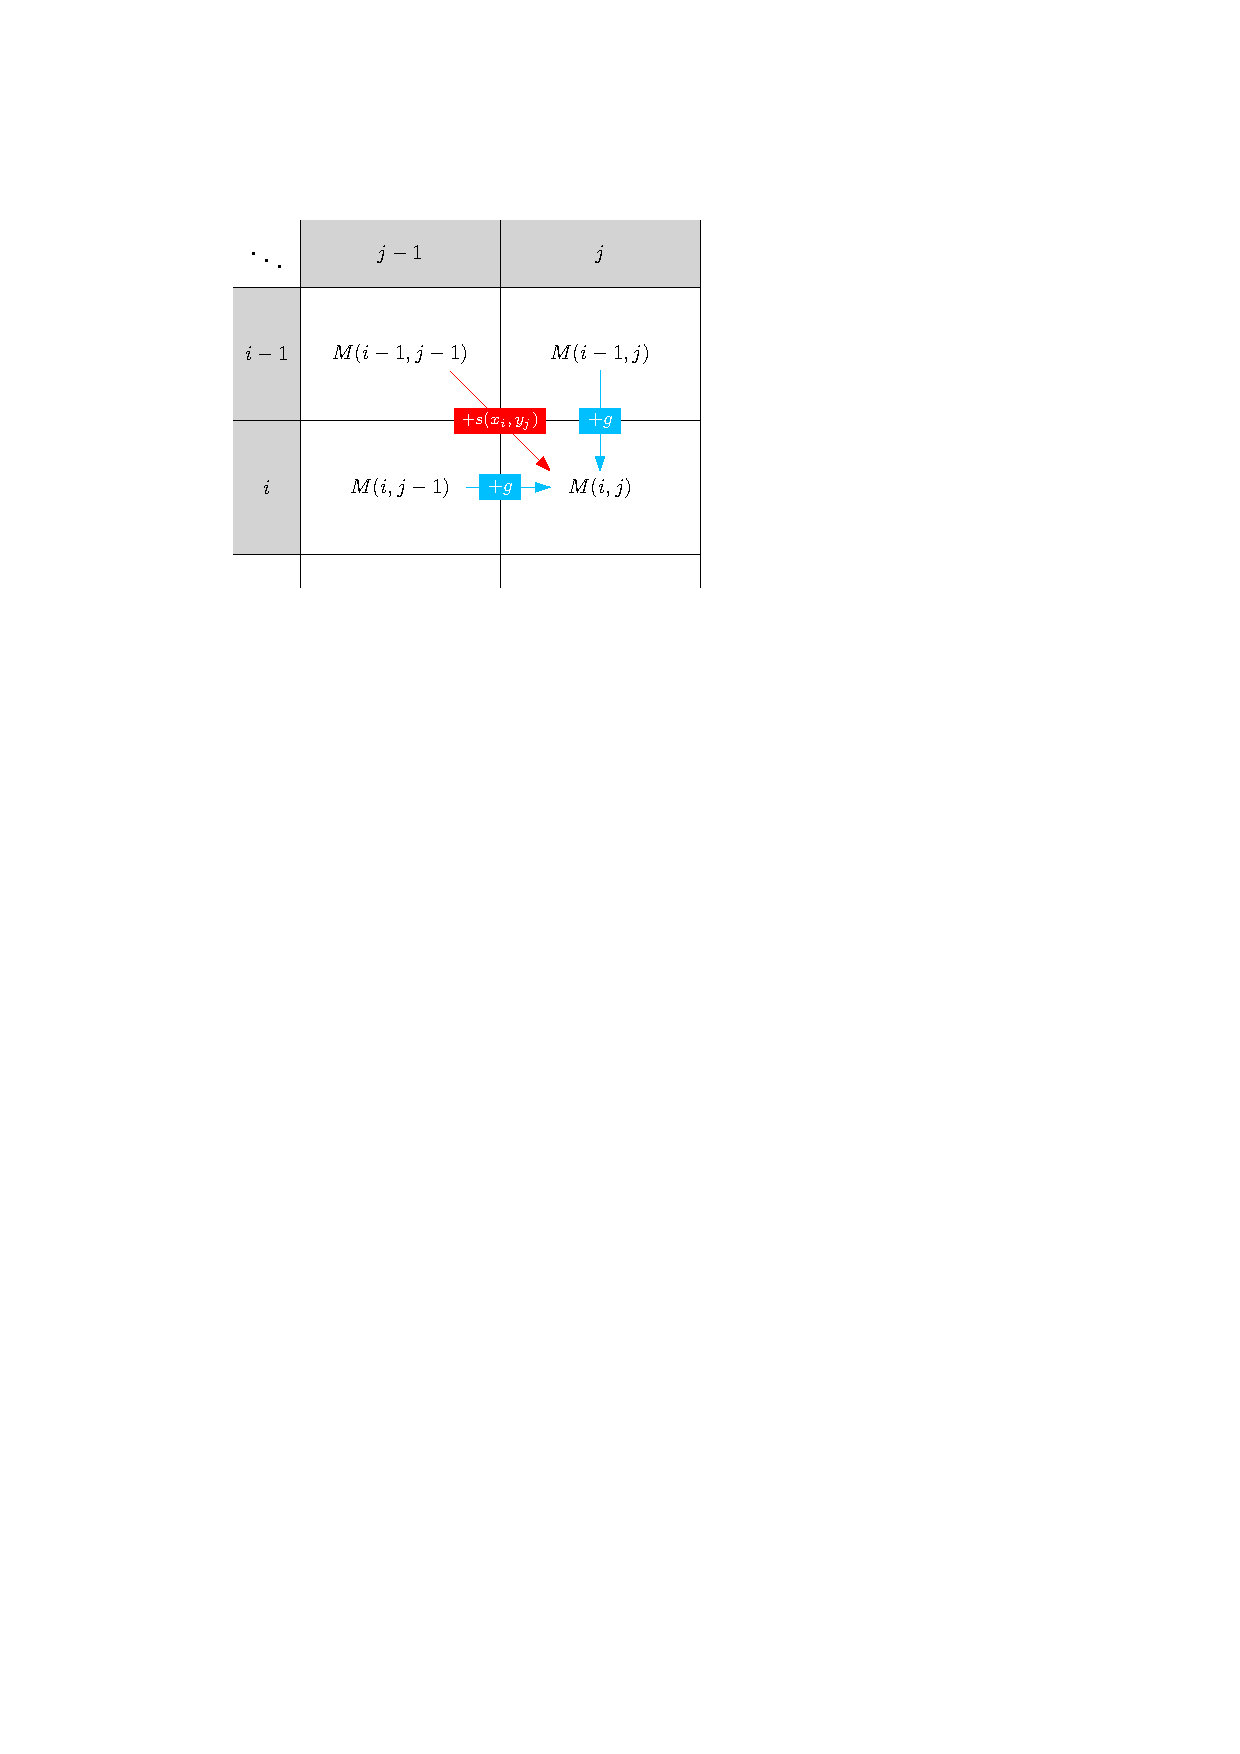
\includegraphics[width=0.4\linewidth]{dp/edit-distance.pdf}
    \caption{The dynamic programming matrix when computing the edit distance. Going diagonally corresponds to a match or substitution; going horizontally and vertically corresponds to insertion and/or deletion.}
    \label{fig:dp-editdistance-mat}
\end{figure}

\part{Network Flow}
\chapter{Ford-Fulkerson}
\section{Flow Network}

\subsection{Definitions}

We can interpret a graph as a ``flow network'' and use it to model the flow of materials such as water through pipes, electricity through wires, or goods through supply chain. Each flow network will have a source where everything originates from and a sink (destination) where everything arrives at. We first formally define a \textbf{flow network}.

\begin{definition}[Flow Network] \index{flow network} \index{source} \index{sink}
    A \textbf{flow network} $G=(V,E)$ is a directed network in which each edge $(u,v) \in E$ has a nonnegative capacity $c(u,v) \geq 0$. Additionally, if $(u,v) \in E$, then $(v,u) \not\in E$. If $(u,v) \not\in E$, then $c(u,v) = 0$.

    In particular, in a flow network, there is a \textbf{source} $s$ and \textbf{sink} $t$, and every vertex lies on some path from from $s$ to $t$. That is, $\forall v \in V$, there exists a path $p$ such that $p = s \leadsto v \leadsto t$.
\end{definition}

\begin{definition}[Flow] \index{flow}
    Let $G=(V,E)$ be a flow network with capacity function $c:\, V\times V \to \R$, and let $s$ be the source and $t$ be the sink of the network. A \textbf{flow} in $G$ is a function $f:\, V\times V \to \R$ that satisfies the following properties:
    \begin{itemize}
        \item Capacity constraint: for all $u,v \in V$, $0 \leq f(u,v) \leq c(u,v)$.
        \item Flow conservation: for all $u \in V - \{s,t\}$, $\sum_{v \in V} f(v,u) = \sum_{v \in V} f(u,v)$. That is, the flow into $u$ must equal the flow out from $u$. When $(u,v) \not\in E$, $f(u,v) = 0$.
    \end{itemize}
    We define the \textbf{value} of a flow $f$ to be
    $$
    |f| = \sum_{v\in V} f(s,v) - \sum_{v \in V} f(v,s)
    $$
    Sometimes, we abuse notations a little bit and omit the summation by writing $f(s,V)$ where $V$ is the set of vertices. Some also uses the notation $f_{in}(v)$ and $f_{out}(v)$ to denote the flow into and out from $v$, respectively.
\end{definition}

\begin{example}[Example of a Flow Network]
    Below is an example of flow network. On each edge $(u,v) \in E$, we write $f(u,v) / c(u,v)$. The slash is simply a separator and does not mean division.

\end{example}

The goal of the maximum flow problem is to find a flow $f$ that maximizes the value of the flow $|f|$. This is also equivalent to finding the maximum flow into the sink $t$.

The max-flow problem is interesting not only because its practical applications, but also its relation to other problems. Many other problems are closely related to the max-flow problem can be polynomial-time reduced to the max-flow problem.

\subsection{Antiparallel Edges and Multiple Sources/Sinks}

In our definition of a flow network, we requires there to be exactly only one source and one sink, and we prohibit antiparallel edges (i.e. if $(u,v) \in E$, then $(v,u) \not\in E$).

However, it is easy to convert a graph with multiple sources and/or sinks and antiparallel edges into a flow network that fit our original definition.

\begin{theorem}
    Suppose that a graph $G$ contains an edge $(u,v)$. We can create a new flow network $G'=(V',E')$ where $V' = V \cup \{x\}$ and $E' = E - \{(u,v)\} \cup \{(u,x),(x,v)\}$. $G'$ is obtained by creating a new vertex $x$ and replacing $(u,v)$ by $(u,x),(v,x)$. We set the capacity $c(u,x) = c(x,v) = c(u,v)$. The maximum flow in $G'$ is the same as the maximum flow in $G$.
\end{theorem}

\begin{proof}
    
\end{proof}

\begin{theorem}
    Let $G$ be a graph with multiple source vertices and multiple sink verticies. Let $G'$ be constructed as follows. Suppose $G$ has sources $S=\{s_1,\ldots,s_i\}$ and sinks $T=\{t_1,\ldots,t_j\}$. We add a supersource $s$ and edges $(s,s_i)$ with capacity $c(s,s_i) = \infty$ for all $s_i \in S$. We add a supersink $t$ and edges $(t_j,t)$ for all $t_j \in T$ with capacity $c(t_j,t) = \infty$. More formally, $G'=(V',E')$ such that $V' = V \cup \{s\} \cup \{t\}$ and $E' = E \cup \{(s,s_i) \mid s_i \in S\} \cup \{(t_j,t) \mid t_j \in T\}$. $G'$ has the same maximum flow as $G$.
\end{theorem}

\begin{proof}
    
\end{proof}

This theorem will become useful later when we look at the maximum bipartite matching problem.

\section{Ford-Fulkerson Method}

Ford-Fulkerson method is a general approach to solve the maximum flow problem. It uses an incremental improve approach by gradually increasing the flow until we reach the maximum. More generally, Ford-Fulkerson can be viewed as a greedy local search algorithm. It is called a method or a scheme because most parts of it can be implemented differently but the general approach remains the same.

The table below summarizes some of the common implementation of the Ford-Fulkerson method. At the end of this chapter, we will discuss the Edmonds-Karp algorithm, and in a later chapter, we will discuss a different algorithm known as the push-relabel algorithm, which uses a different approach than Ford-Fulkerson.

\begin{table}[htpb]
    \centering
    \begin{tabular}{c|c|c}
    Algorithm & Implementation & Complexity \\
    \hline
    Edmonds-Karp (1970) & BFS for finding augmenting path & $O(|E|^2|V|)$ \\
    Dinitz (1970) & BFS + DFS for finding augmenting path & $O(|V|^2 |E|)$ \\
    Capacity Scaling (Dinitz, 1972) & Capacity scaling heuristic & $O(|E|^2 \log c_{max})$ \\
    Dinitz-Gabow (1973) & Capacity scaling heuristic & $O(|V||E| \log c_{max})$ 
    \end{tabular}
    \caption{Comparison of multiple algorithms based on the Ford-Fulkerson. $c_{max}$ in capacity scaling denotes the largest capacity in the network.}
    \label{tab:ford-fulkerson}
\end{table}

\subsection{Idea Behind Ford-Fulkerson}

The idea behind Ford-Fulkerson is quite simple. For each iteration of the algorithm, we find a path from $s$ to $t$, increase the flow along the path until we hit a bottleneck at one of the edges on the path (the edge with the smallest remaining capacity). This is called augmenting flow, and the path is called augmenting path. When augmenting the flow along the augmenting path, we may also want to decrease the flow along each residue (i.e. reverse) edge so that we can ``undo'' bad augmentation choices. We will show that when the algorithm terminates, it correctly returns the max-flow.

Note that this is more precisely, only the partial correctness. Surprisingly, depending on the implementation and capacities, the algorithm may not terminate. In particular, the Ford-Fulkerson method may fail to terminate if edge capacities are irrational \cite{Zwick-FF-Example}. In his 1993 paper, Zwick showed a minimal example flow network (with 6 vertices and 8 edges) on which Ford-Fulkerson fails to terminate.

\begin{codebox}
    \Procname{$\proc{Ford-Fulkerson}(G,s,t)$}
    \li $f = 0$ for all $(u,v) \in E$ 
    \li \While there exists an augmenting path $p$ in residue network $G_f$ \Do
        \li augment flow $f$ along $p$
    \End
    \li \Return $f$
\end{codebox}

\section{Correctness of Ford-Fulkerson}

\subsection{Residue Network and Augmentation}

Let us make the idea more concrete by formalizing it and proving the correctness of the Ford-Fulkerson method. We first define what a residue network is.

Given a flow network $G$, the residue network $G_f$ contains edges with capacities that represent how much more flow we can push through each edge. For each edge $(u,v)$, we will also add backward edges $(v,u)$ to the residue network that can at most cancel out the flow through the edge $(u,v)$.

\begin{definition}[Residue Capacity] \index{residue capacity}
    Let $G=(V,E)$ be a flow network with source $s$ and sink $t$. Let $f$ be a flow in $G$, and consider a pair of vertices $u,v \in V$. The \textbf{residue capacity} $c_f(u,v)$ is defined as
    $$
    c_f(u,v) = \begin{cases}
        c(u,v) - f(u,v) & (u,v) \in E \\
        f(v,u) & (v,u) \in E \\
        0 & \text{otherwise}
    \end{cases}
    $$
    By assumption, since $G$ is a flow network, $(u,v) \in E \iff (v,u) \not\in E$, exactly one case in the definition applies.
\end{definition}

\begin{definition}[Residue Network] \index{residue network}
    Let $G=(V,E)$ be a flow network and a flow $f$. The \textbf{residue network} of $G$ induced by $f$, denoted $G_f$ is $G_f = (V,E_f)$ where $E_f = \{(u,v) \in V \times V \mid c_f(u,v) > 0 \}$.
\end{definition}
A residue network contains at most twice many edges as the original flow network. If an edge does not exist in $G$ (has zero capacity), it does not exist in $G_f$ either.

\begin{definition}[Augmentation] \index{augmentation (max-flow)}
    Let $G=(V,E)$ be a flow network with flow $f$. $G_f$ is the residue network of $G$ induced by $f$. Suppose that $f'$ is a flow in $G_f$. We define the \textbf{augmentation} of $f$ by $f'$, denoted $f \uparrow f'$, to be a function $(f \uparrow f'):\, V\times V \to \R$ such that
    $$
    (f \uparrow f')(u,v) = \begin{cases}
        f(u,v) + f'(u,v) - f'(v,u) & (u,v) \in E \\
        0 & \text{otherwise}
    \end{cases}
    $$
\end{definition}

Note that because we allow backward edges in a residue network, we need to subtract $f'(v,u)$ when augmenting $f$ and $f'$ on edge $(u,v)$. The notion of pushing flow through a reverse edge is called cancellation.

\begin{lemma} \label{lem:value-of-augmented-flow}
    Let $G=(V,E)$ be a flow network with source $s$ and sink $t$, and let $f$ be a flow in $G$. Let $G_f$ be the residue network of $G$ induced by $f$, and let $f'$ be a flow in $G_f$. Then $f \uparrow f'$ is a flow in $G$ and $|f \uparrow f'| = |f| + |f'|$.
\end{lemma}

\begin{proof}
    To show that $f \uparrow f'$ is a flow in $G$, it suffices to show the capacity constraint and flow conservation properties hold.

    Capacity constraint: Let $u,v \in V$. Then, \\ $(f \uparrow f')(u,v)=f(u,v)+f'(u,v)-f'(v,u) \leq f(u,v) + f'(u,v) \leq f(u,v) + c_f(u,v) = f(u,v) + c(u,v) - f(u,v) = c(u,v)$.

    Flow conservation: Fix $u \in V$. Let $In(u) = \{v \in V \mid (u,v) \in E\}$ and $Out(u) = \{v \in V \mid (u,v) \in E\}$. That is, $In(u)$ is the set of vertices with edges to $u$ and $Out(u)$ is the set of vertices with edges from $u$.
    $$
    \begin{aligned}
        \sum_{v \in Out(u)} (f \uparrow f')(u,v) - \sum_{v \in In(u)} (f \uparrow f')(v,u) =&
        \sum_{v \in Out(u)} f(u,v) + \sum_{v \in Out(u)} f'(u,v) - \sum_{v \in Out(u)} f'(v,u) - \\
        & \sum_{v \in In(u)} f(v,u) - \sum_{v \in In(u)} f'(v,u) + \sum_{v \in In(u)} f'(u,v)
    \end{aligned}
    $$
    Regrouping the terms yields \\ $\sum_{v \in Out(u)} f(u,v) - \sum_{v \in In(u)} f(v,u) + [\sum_{v \in Out(u)} f'(u,v) + \sum_{v \in In(u)} f'(u,v) ] \\ - [ \sum_{v \in Out(u)} f'(v,u) + \sum_{v \in In(u)} f'(v,u) ]$,
    
    which is equivalent to $\sum_{v \in V} f(u,v) - \sum_{v \in V} f(v,u) + \sum_{v \in V} f'(u,v) - \sum_{v \in V} f'(v,u)$. We can extend the summation from $In(u)$ and $Out(u)$ to $V$ because all the additional terms are 0 by definition of flow and the fact that there $(u,v) \not\in E$ for $v \in V-Out(u)$ and $(v,u) \not\in E$ for $v \in V-In(u)$.

    By flow conservation of $f$ and $f'$ individually, \\
    $\sum_{v \in V} f(u,v) - \sum_{v \in V} f(v,u) + \sum_{v \in V} f'(u,v) - \sum_{v \in V} f'(v,u) = 0$, \\
    which implies that $\sum_{v \in Out(u)} (f \uparrow f')(u,v) = \sum_{v \in In(u)} (f \uparrow f')(u,v)$.

    To show that $|f \uparrow f'| = |f| + |f'|$, set $u = s$ in the previous derivation, and we have
    $$
    \begin{aligned}
        |f \uparrow f'| &= \sum_{v \in Out(s)} (f \uparrow f')(s,v) - \sum_{v \in In(s)} (f \uparrow f')(v,s) \\
        &= \sum_{v \in V} f(s,v) - \sum_{v \in V} f(v,s) + \sum_{v \in V} f'(s,v) - \sum_{v \in V} f'(v,s) \\
        &= |f| + |f'|.
    \end{aligned}
    $$
\end{proof}

\subsection{Augmenting Paths}

\vspace{\parskip}

\begin{definition}[Augmenting Path] \index{augmenting path}
    Given a flow network $G=(V,E)$ with source $s$ and sink $t$ and flow $f$, an \textbf{augmenting path} $p$ is a simple path from $s$ to $t$ in the residue graph $G_f$ of $G$ induced by $f$.
\end{definition}

\begin{definition}[Residue Capacity of an Augmenting Path]
    Let $p$ be an augmenting path for the flow network $G$. Then, the \textbf{residue capacity} of $p$ is defined as the maximum amount by which we can increase the flow on each edge in the $p$, or more formally,
    $$
    c_f(p) = \min \{c_f(u,v) \mid \text{$(u,v)$ is on $p$} \}
    $$
\end{definition}

\begin{definition}[Flow of an Augmenting Path]
    Let $G=(V,E)$ be a flow network, $f$ be a flow in $G$, and let $p$ be an augmenting path in $G_f$. Define the flow of the augmenting path $f_p:\, V \times V \to \R$ by
    $$
    f_p(u,v) = \begin{cases}
        c_f(p) & \text{$(u,v)$ on $p$} \\
        0 & \text{otherwise}
    \end{cases}
    $$
\end{definition}

\begin{lemma} \label{lem:augmenting-flow}
    The flow $f_p$ on an augmenting path $p$ is a flow in $G_f$ with value $|f_p| = c_f(p) > 0$.
\end{lemma}

\begin{proof}
    We show that $f_p$ satisfies the capacity constraint and flow conservation.

    Capacity constraint: If $(u,v)$ is on $p$, then $f_p(u,v)=c_f(p) \leq c_f(u,v)$ by definition. If $(u,v)$ is not on $p$, then $f_p(u,v) = 0 \leq c_f(p)$.

    Flow conservation: Fix $u \in V - \{s,t\}$. First, consider the case where $u$ is on $p$. Say, edges $(w,u)$ and $(u,v)$ are on $p$. Then, since $p$ is a simple path and $u \in V-\{s,t\}$, there is exactly one edge going into and out from $u$. $\sum_{v \in In(u)} f_p(v,u) = f_p(w,u) = c_f(p)$ and $\sum_{v \in Out(u) f_p(u,v)} = f_p(u,v) = c_f(p)$. If $(u,v)$ is not on $p$, both the flow into $u$ and flow out from $u$ are 0. In both cases, flow conservation is satisfied.

    Finally, to show that $|f_p| = c_f(p)$, consider the flow out from $s$. Since $p$ is a simple path, there is no flow input $s$, so $|f_p| = \sum_{v \in V} f(s,v) - \sum_{v \in V} f(v,s) = c_f(p) - 0 = c_f(p)$ 
\end{proof}

Immediately following from Lemma \ref{lem:augmenting-flow} and \ref{lem:value-of-augmented-flow}, we have the following corollary.

\begin{corollary} \label{corollary:augmentation-increases-flow}
    Let $G=(V,E)$ be a flow network, let $f$ be a flow in $G$, and let $p$ be an augmenting path in $G_f$. Let $f_p$ be a flow on the augmenting path defined previously. Then, $f \uparrow f_p$ is a flow in $G$ with value
    $$
    |f \uparrow f_p| = |f| + |f_p| > |f|
    $$
\end{corollary}

\begin{proof}
    By Lemma \ref{lem:value-of-augmented-flow}, $|f_p| = c_f(p) > 0$. By Lemma \ref{lem:augmenting-flow}, $f \uparrow f_p$ is a flow and has value $|f|+|f_p| > |f|$.
\end{proof}

As a result of Corollary \ref{corollary:augmentation-increases-flow}, we know that augmenting a flow with an augmenting path yields a flow with value strictly greater than the flow prior to augmentation.

\subsection{Max-Flow Min-Cut Theorem}

Our analyses so far shows a promising picture of the correctness of the Ford-Fulkerson method. By iteratively augmenting $f$ with an augmenting path $p$, we gradually increases the flow in the flow network, and when the procedure halts, we should expect to see that $f$ is equal to the maximum flow. The proof utilizes the max-flow min-cut theorem and shows that if there is no augmenting path, there exists a cut in the flow network that implies that $f$ is the max-flow.

\begin{definition}[Cut and Net Flow Across a Cut] \index{cut} \index{minimum cut}
    A \textbf{cut} $(S,T)$ of flow network $G=(V,E)$ is a partition of $V$ into $S$ and $T=V-S$ such that $s \in S$ and $t \in T$. If $f$ is a flow, then the \textbf{net flow} $f(S,T)$ across the cut $(S,T)$ is defined as
    $$
    f(S,T) = \sum_{u \in S}\sum_{v \in T} f(u,v) - \sum_{u \in S}\sum_{v \in T} f(v,u)
    $$
    The \textbf{capacity of the cut}, denoted $c(S,T)$ is
    $$
    c(S,T) = \sum_{u \in S}\sum_{v \in T} c(u,v)
    $$
\end{definition}
A \textbf{minimum cut} is a cut whose capacity is minimum over all cuts of the flow network. The definition of a cut and minimum cut will help us prove the important max-flow min-cut theorem. The proof roughly follows the outline shown in Figure \ref{fig:maxflow-ford-fulkerson-proof}.

\begin{figure}[htbp]
    \centering
    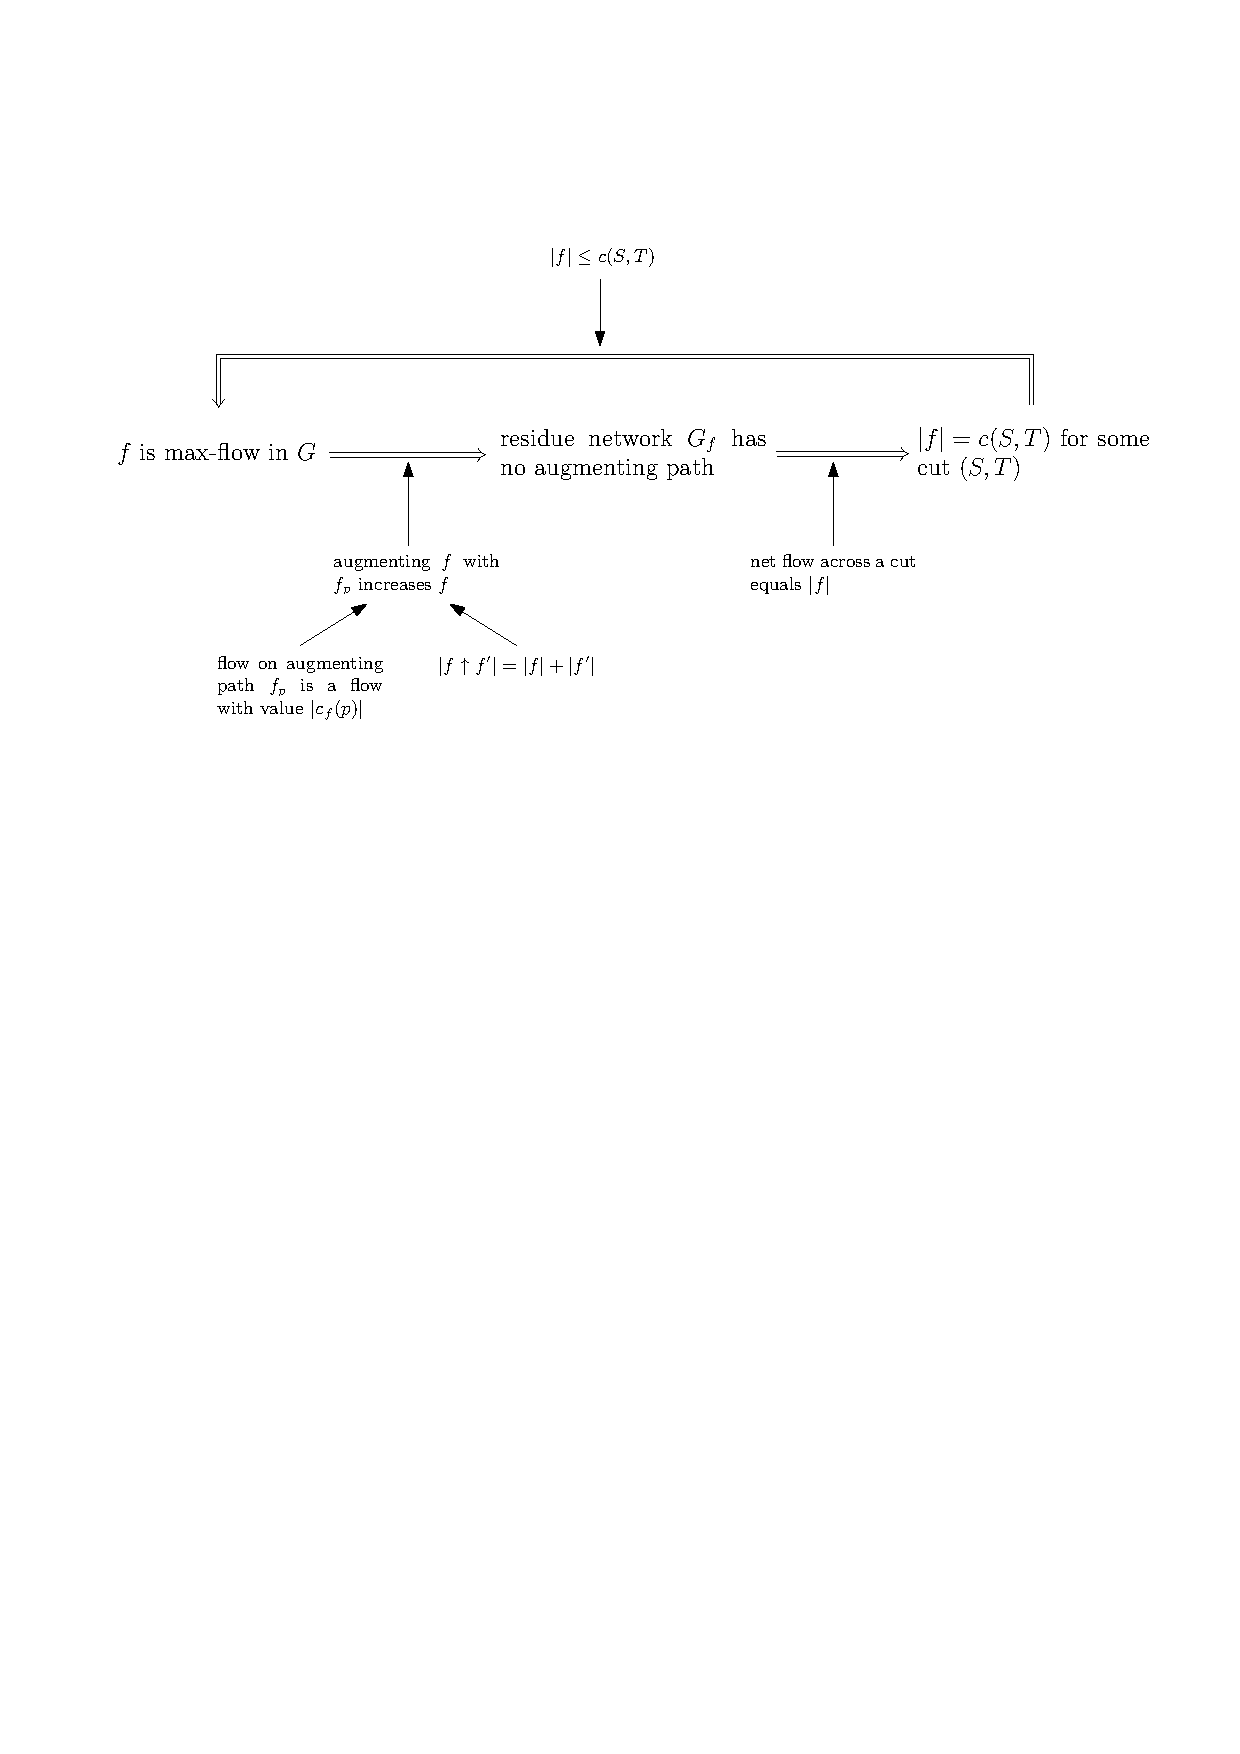
\includegraphics[width=0.95\linewidth]{maxflow/maxflow-mincut-proof-outline.pdf}
    \hfill
    \caption{Proof outline for the partial correctness of the Ford-Fulkerson method.}
    \label{fig:maxflow-ford-fulkerson-proof}
\end{figure}

\begin{lemma} \label{lem:flow-across-cut}
    Let $f$ be a flow in a flow network $G$ with source $s$ and sink $t$. Let $(S,T)$ be a cut of $G$. Then, the net flow across the cut $(S,T)$ is $f(S,T) = |f|$.
\end{lemma}

\begin{proof}
    Let $(S,T)$ be a cut in $G$. Consider the following net flows:
    \begin{itemize}
        \item $f(S,T)$: the net flow across the cut $(S,T)$ 
        \item $f(S,V)$: the net flow for edges starting in $S$
        \item $f(S,S)$: the net flow within $S$ 
        \item $f(\{s\},V)$: the net flow from $s$ (i.e. $|f|$)
        \item $f(S-\{s\},V)$: the net flow of edges that start from the partition $S$ but not the source $s$ 
    \end{itemize}
    Fix $u \in V - \{s,t\}$. By flow conservation, we have $\sum_{v \in V} f(u,v) - \sum_{v \in V} f(v,u) = 0$. This is true for all $u \in V - \{s,t\}$, so 
    $$\sum_{u \in S-\{s\}} \left(\sum_{v \in V} f(u,v) - \sum_{v \in V} f(v,u)\right) = 0.$$ 
    
    This summation can be expanded to 
    $$\sum_{u \in S-\{s\}}\sum_{v \in V} f(u,v) - \sum_{u \in S-\{s\}}\sum_{v \in V} f(v,u) = 0$$
    by linearity. Note this expression is equivalent to $f(S-\{s\},V)$ by definition. So, $f(S-\{s\},V) = 0$.

    Now consider $f(S,S)$. By definition, we can rewrite $f(S,S)$ as 
    $$\sum_{u \in S}\sum_{v \in S} f(u,v) - \sum_{u \in S}\sum_{v \in S} f(v,u) = 0$$
    because for all vertices $x,y \in S$, the term $f(x,y)$ appears exactly once in each summation. Hence, $f(S,S) = 0$.

    Since $V = S \cup T$ and $S \cap T = \emptyset$,
    $$
    \begin{aligned}
        f(S,T) &= f(S,V) - f(S,S) \\
        &= f(S,V) \\
        &= f(\{s\},V) + f(S-\{s\},V) \\
        &= f(\{s\},V) \\
        &= |f|
    \end{aligned}
    $$ 
\end{proof}
This proof is inspired by the proof presented in the second edition of CLRS. The proof in the third edition employs a more rigorous argument using properties of summation, but I personally find it less intuitive.

A corollary to this lemma shows that cut capacity can be used to bound the value of a flow.

\begin{corollary} \label{corollary:flow-upper-bound}
    The value of any flow $f$ in a flow network $G$ is bounded above by the capacity of any cut of $G$.
\end{corollary}

\begin{proof}
    Let $(S,T)$ be a cut of $G$ and let $f$ be a flow. By Lemma \ref{lem:flow-across-cut} and capacity constraint,
    $$
    \begin{aligned}
        |f| = f(S,T) &= \sum_{u \in S}\sum_{v \in T}f(u,v) - \sum_{u \in S}\sum_{v \in T}f(v,u) \\
        &\leq \sum_{u \in S}\sum_{v \in T}f(u,v) \\
        &\leq \sum_{u \in S}\sum_{v \in T} c(u,v) & \text{capacity constraint} \\
        &= c(S,T) & \text{definition}
    \end{aligned}
    $$
\end{proof}

Now we finally have everything we need to prove the max-flow min-cut theorem. We will follow the proof outline to prove the equivalences (iff).

\begin{theorem}[Max-Flow Min-Cut Theorem] \index{max-flow min-cut theorem}
    If $f$ is a flow in a flow network $G=(V,E)$ with source $s$ and sink $t$, then the following conditions are equivalent
    \begin{enumerate}
        \item $f$ is a maximum flow in $G$ 
        \item The residue network $G_f$ contains no augmenting paths
        \item $|f| = c(S,T)$ for some cut $(S,T)$ of $G$ 
    \end{enumerate}
\end{theorem}

\begin{proof}
    \hfill

    (1) $\Rightarrow$ (2): Suppose, for contradiction, that $f$ is a maximum flow in $G$, but $G_f$ has a new augmenting path $p$. Then, by Corollary \ref{corollary:augmentation-increases-flow}, the flow obtained by augmenting $f$ and $f_p$ has a strictly greater value and $f \uparrow f_p$ is a flow in $G$. This contradicts the assumption that $f$ is a maximum flow. 

    (2) $\Rightarrow$ (3): Assume (2) holds. Then, there is no path from $s$ to $t$ in the residue network $G_f$. Let $S = \{ v \in V \mid \text{there exists a path from $s$ to $v$ in $G_f$} \}$, and let $T = V-S$. Clearly, $(S,T)$ is a cut (this can be trivially proved by showing $s \in S$ and $t \not\in S$ because there is no path from $s$ to $t$). We claim that for each $u\in S$ and $v \in T$, $(u,v) \in E$, $f(u,v) = c(u,v)$. To see why this is true, we use proof by contradiction. Suppose the claim is false. By capacity constraint $f(u,v) \leq c(u,v)$. If $f(u,v) \neq c(u,v)$, $f(u,v) < c(u,v)$ and $(u,v) \in E_f$ because it would have positive residue capacity. But then, this means there would be a path from $u$ to $v$ and $v \in S$, contradicting the assumption that $v \in T$. The other case where $(v,u) \in E$ follows from the same argument with $u$ and $v$ swapped.

    (3) $\Rightarrow$ (1): Assume (3) holds. Then, there exists a cut $(S,T)$ such that $|f| = c(S,T)$. By Corollary \ref{corollary:flow-upper-bound}, $|f| \leq c(S,T)$. This implies that every other flow has value less than $f$, so $f$ is a maximum flow.
\end{proof}

This theorem shows that if Ford-Fulkerson terminates, then the resulting flow is the maximum flow. The proof of correctness also suggests the following algorithm that elaborates on the Ford-Fulkerson method outline described earlier.

\begin{codebox}
    \Procname{$\proc{Ford-Fulkerson}(G=(V,E),s,t)$}
    \li \For each $(u,v) \in E$ \Do
        \li $(u,v).f = 0$ \RComment{initialize flow to 0}
    \End
    \li \While there exists a path $p$ from $s$ to $t$ in the residue network $G_f$ \Do
        \li $c_f(p) = \min \{c_f(u,v) \mid \text{$(u,v)$ is on $p$} \}$ \RComment{residue capacity of path $p$}
        \li \For each $(u,v)$ on $p$ \Do \RComment{augment flow}
            \li \If $(u,v) \in E$ \Then
                \li $(u,v).f = (u,v).f + c_f(p)$
            \li \Else $(v,u).f = (v,u).f - c_f(p)$
            \End
        \End
    \End
\end{codebox}

The runtime of Ford-Fulkerson's algorithm/method depends on the way we implement the procedure for finding augmenting path $p$. In the next chapter, we will look at Edmonds-Karp's algorithm, which implements this operation using BFS.

\chapter{Edmonds-Karp Algorithm}
\section{Edmonds-Karp} \index{Edmonds-Karp algorithm}

In the last chapter, we saw the Ford-Fulkerson method for finding the maximum flow. We have left out one important aspect of the implementation -- how to find the augmenting path. The \textit{\textbf{Edmonds-Karp algorithm}} finds augmenting paths using breadth-first search (BFS). We will first take a look at the pseudocode for Edmonds-Karp. It follows the same structure as Ford-Fulkerson.

\begin{codebox}
    \Procname{$\proc{Edmonds-Karp}(G=(V,E),s,t)$}
    \li \For each $(u,v) \in E$ \Do
        \li $(u,v).f = 0$ \RComment{initialize flow to 0}
    \End
    \li $p = \proc{BFS}(G_f, s, t)$ \RComment{find shortest path from $s$ to $t$ on residue network}
    \li \While $p \neq \const{nil}$ \Do
        \li $c_f(p) = \min \{c_f(u,v) \mid \text{$(u,v)$ is on $p$} \}$ \RComment{residue capacity of path $p$}
        \li \For each $(u,v)$ on $p$ \Do \RComment{augment flow}
            \li \If $(u,v) \in E$ \Then
                \li $(u,v).f = (u,v).f + c_f(p)$
            \li \Else $(v,u).f = (v,u).f - c_f(p)$
            \End
        \End
        \li $p = \proc{BFS}(G_f,s,t)$ 
    \End
\end{codebox}

The correctness of the Edmonds-Karp algorithm follows immediately from the correctness of Ford-Fulkerson.

\section{Running Time of Edmonds-Karp Algorithm}

We will show that the Edmonds-Karp algorithm runs in $O(|V||E|^2)$ time. It is a rather subtle proof involving properties of shortest paths and how augmenting a path on the residue network affects the shortest path from $s$ to $t$.

\begin{lemma} \label{lem:edmondskarp-runtime-1}
    Let $\delta_f(s,v)$ be the shortest-path distance from $s$ to $v$ in the residue network $G_f$. After each flow augmentation, $\delta_f(s,v)$ does not decrease for all $v \in V - \{s,t\}$.
\end{lemma}

\begin{proof}
    Suppose for contradiction, that there exists some vertex $v \in V-\{s,t\}$ such that $\delta_f(s,v)$ is decreased after certain flow augmentation. Let $f$ be the flow before the augmentation, and $f'$ be the flow immediately after the augmentation. Let $v$ be the vertex with \textbf{minimum} $\delta_{f'}(s,v)$ whose distance was decreased by flow augmentation. Further, let $u$ be the vertex immediately before $v$ on the shortest path from $s$ to $v$ in $G_{f'}$. By our assumption, $\delta_{f'}(s,v) < \delta_f (s,v)$.

    Since we have chosen $v$ to be the vertex with minimum $\delta_{f'}(s,v)$ whose flow was decreased, we know that the distance from $s$ to $u$ (the vertex immediately before $v$ on the shortest path from $s$ to $v$ in $G_{f'}$) did not decrease. Hence,
    $$
    \delta_{f}(s,u) \leq \delta_{f'}(s,u)
    $$

    \textit{Claim}. $(u,v) \not\in G_f$.

    We can prove this claim by contradiction. Suppose not. Then, since $\delta_{f}(s,v)$ is the shortest-path distance from $s$ to $v$ in $G_f$, by the triangle inequality,
    $$
    \delta_f (s,v) \leq \delta_f (s,u) + 1 \leq \delta_{f'}(s,u) + 1 = \delta_{f'}(s,v)
    $$
    which is a contradiction to our assumption that $\delta_{f'}(s,v) < \delta_f (s,v)$. 

    The only way $(u,v) \not\in G_f$ and $(u,v) \in G_{f'}$ after one augmentation step is if the flow through $(v,u)$ is increased during the augmentation (creating the reverse edge $(u,v)$). Since Edmonds-Karp algorithm uses BFS to select augmenting paths, this implies that $(v,u)$ is on the shortest path selected by the algorithm. But then, 
    $$
    \delta_f(s,v) = \delta_f(s,u) - 1 \leq \delta_{f'}(s,u) - 1 = \delta_{f'}(s,v) - 1 - 1
    $$
    which implies that $\delta_f(s,v) < \delta_{f'}(s,v)$, contradicting our assumption that $\delta_{f'}(s,v) < \delta_f(s,v)$.
\end{proof}

We say an edge is \textit{\textbf{critical}} on an augmenting path $p$ if $c_f(p) = c_f(u,v)$ (i.e. $(u,v)$ is the bottleneck). Based on our algorithm, during an augmentation of the path $p$, $(u,v)$ is removed and $(v,u)$ is added to the residue network.

\begin{lemma} \label{lem:edmondskarp-runtime-2}
    Between any two steps in which $(u,v)$ is critical, $\delta(s,u)$ increases by at least 2.
\end{lemma}

\begin{proof}
    Suppose $(u,v)$ was cirtical in $G_f$. So, $(u,v)$ is removed after augmentation. Further, since $(u,v)$ is selected by the algorithm, it must be on the shortest path from $s$ to $t$, so
    $$
    \delta_f(s,v) = \delta_f(s,u) + 1
    $$
    Once $(u,v)$ is removed, it can only reappear in a residue network if the flow from $u$ to $v$ is decreased, which is only possible when $(v,u)$ is in the network. Let $f'$ be the flow immediately before the augmentation that added $(u,v)$ back. Then, the algorithm must have selected an augmenting path containing $(v,u)$. By Lemma \ref{lem:edmondskarp-runtime-1} on $v$, $\delta_{f}(s,v) \leq \delta_{f'}(s,v)$. It follows that
    $$
    \delta_{f'}(s,u) = \delta_{f'}(s,v) + 1 \geq \delta_{f}(s,v) + 1 = \delta_{f}(s,u) + 2
    $$
    Hence, between the two steps in which $(u,v)$ is critical, the distance from $s$ to $u$ increases by at least 2.
\end{proof}

\begin{corollary} \label{lem:edmondskarp-runtime-3}
    Every edge can become critical at most $|V|/2$ times.
\end{corollary}

\begin{proof}
    Immediate from \ref{lem:edmondskarp-runtime-2}. After the first time an edge $(u,v)$ became critical, the distance of the vertex from $s$ to $u$ increases by at least 2 every time, and there are $|V|-2$ vertices that can show up on the shortest path from $s$ to $u$. This can happen at most $(|V|-2)/2$ times. Along with the first time $(u,v)$ becmoes critical, we have in total at most $|V|/2$ times.
\end{proof}

\begin{theorem}
    \proc{Edmonds-Karp} runs in $O(|V||E|^2)$ time.
\end{theorem}

\begin{proof}
    As shown by Corollary \ref{lem:edmondskarp-runtime-3}, there can be at most $O(|V||E|)$ augmentations steps because there are $|E|$ edges, and every edge can be critical for at most $|V|/2 \in O(|V|)$ times. Each augmentation step takes $O(|E|)$ using breadth-first search and hence the running time $O(|V||E|^2)$.
\end{proof}

\chapter{Maximum Bipartite Matching and Applications of Network Flow}
\section{Maximum Bipartite Matching} \index{bipartite graph} \index{maximum bipartite matching}

Given a \textit{\textbf{bipartite graph}} $G=(V,E)$ where $V = V_1 \cup V_2$ for some $V_1 \cap V_2 = \emptyset$ and $E \subseteq V_1 \times V_2$, a matching is a set of edges going from vertices in $V_1$ to vertices in $V_2$. The objective of the \textit{\textbf{maximum bipartite matching problem}} is to find a bipartite matching of the maximum cardinality.

There is a natural way to solve this problem using max flow. Given such bipartite graph, we can add a source node $s$ and target node $t$ and for all $u \in V_1$, add edge $(s,u)$ with capacity 1 and for all $v \in V_2$, add edge $(v,t)$ with capacity 1. Assign a capacity of 1 to all other edges already in $E$ (note that technically we need to turn those undirected edges into direct edges going from $V_1$ to $V_2$ but the construction for this is trivial so we won't spend time describing it formally).

\begin{figure}[htbp]
    \centering
    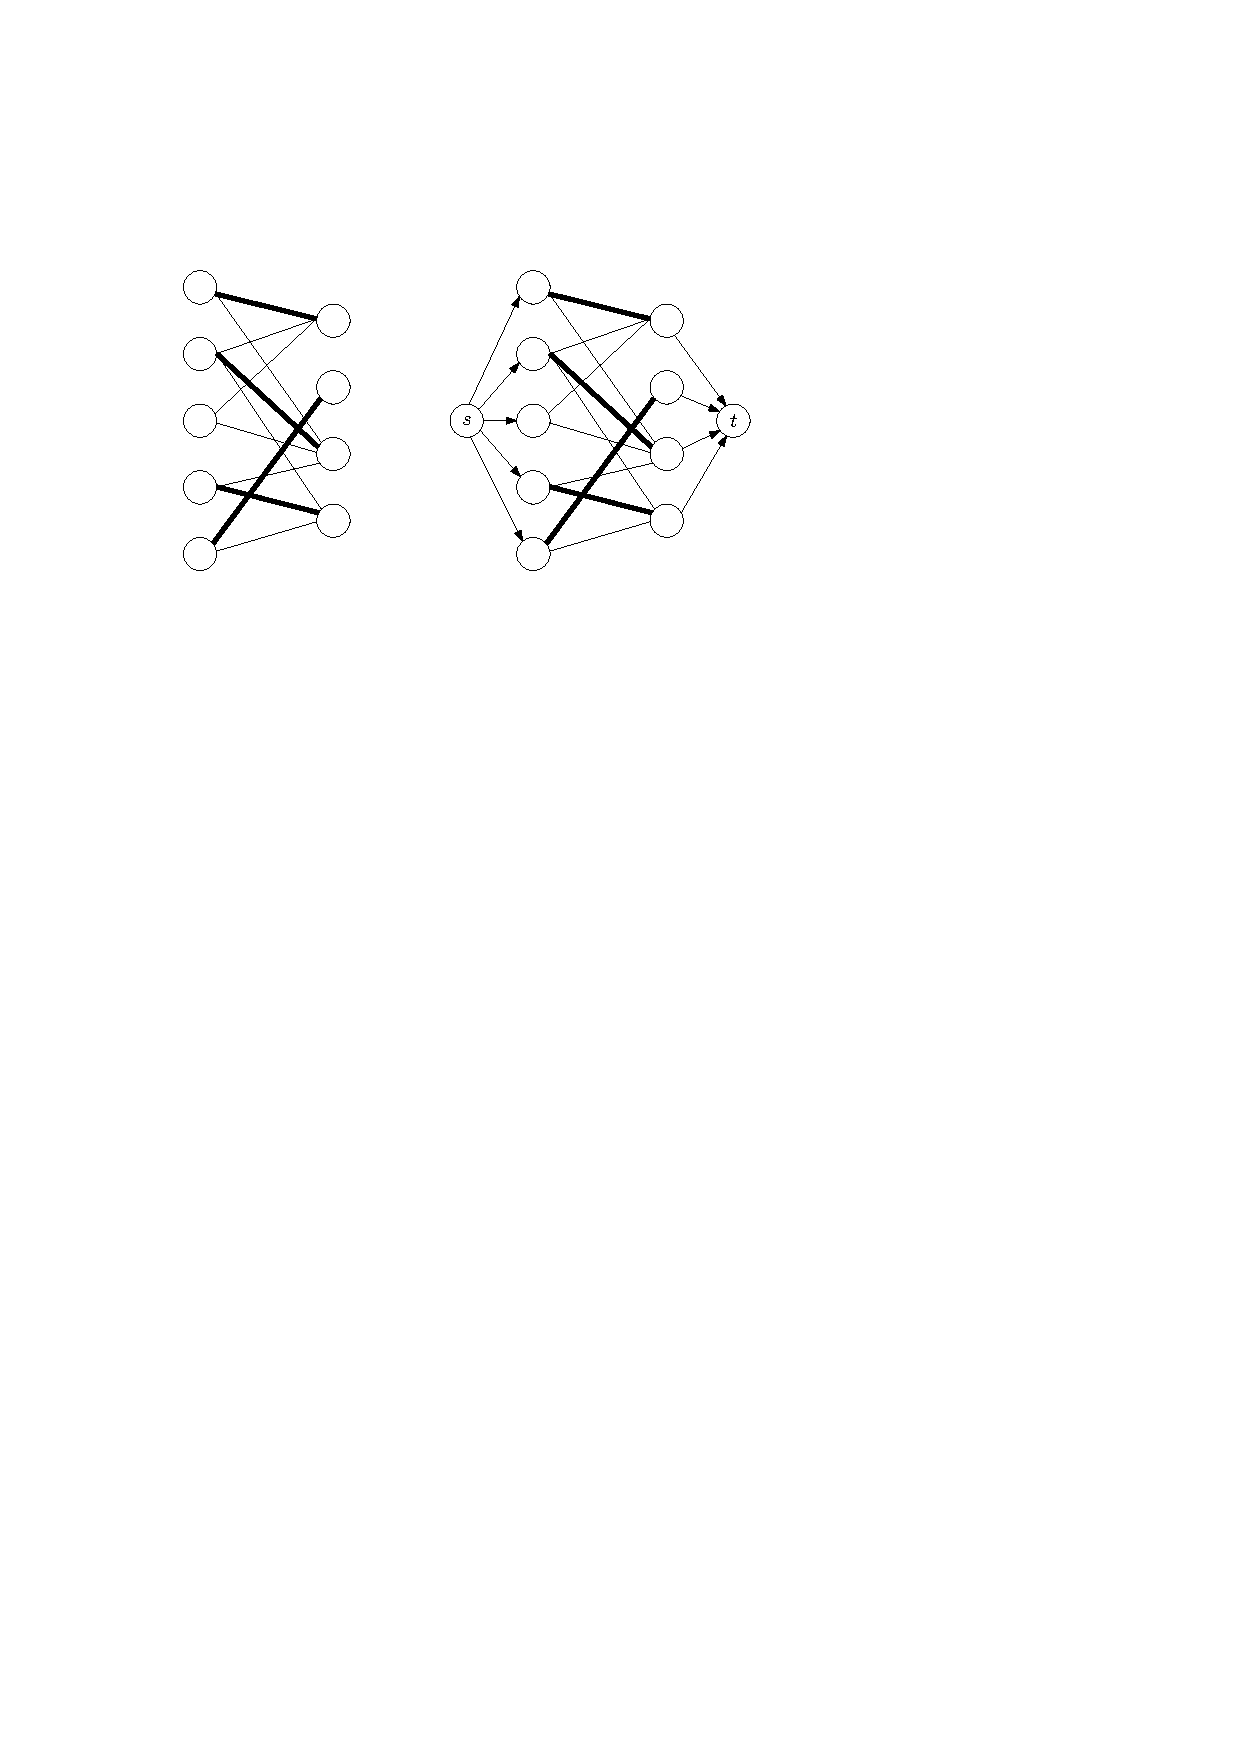
\includegraphics[width=0.7\linewidth]{maxflow/bipartite-matching.pdf}
    \caption{Maximum bipartite matching and its reduction to maximum flow problem.}
    \label{fig:maximum-bipartite-matching}
\end{figure}

Once we apply this construction to obtain a flow network, we can run any max-flow algorithms and the result gives rise to a matching with the maximum cardinality.

\begin{theorem}[Integrality Theorem] \index{integrality theorem}
    If the capacities in a flow network are integers, then the value of the maximum flow produced by the Ford-Fulkerson method is also an integer.
\end{theorem}

\begin{proof}
    By induction on the number of augmentations.
\end{proof}

Once we have the integrality theorem, we are able to prove the corrctness of the reduction from maximum bipartite matching to max flow. We do so by showing that there is an one-to-one correspondence between matchings of size $k$ in the original graph and flows of value $k$ in the flow network.

\begin{proof}
    \hfill

    (matching $\Rightarrow$ integral flow): Let $M = \{(u_1,v_1),\ldots,(u_k,v_k)\}$ be a matching of size $k$. We construct a flow $f$ such that for all $i = 1,\ldots,k$, $f(s,u_i) = f(u_i,v_i) = f(v_i,t) = 1$. It is easy to verify that $f$ is indeed a flow (by showing that it satisfies capacity constraint and flow conservation). The value of the flow $|f| = \sum_{v \in V}f(s,v) - \sum_{v \in V}(v,s) = k$.

    (integral flow $\Rightarrow$ matching): Let $f$ be a flow with value $k$. Let $M$ be the matching such that
    $$
    M = \{(u,v) \in E \mid u \in V_1,\,v \in V_2,\,f(u,v) = 1\}.
    $$
    Since a flow of $k$ comes out of $s$, there must be $k$ edges each with flow of 1 going from $s$ to distinct vertices in $V_1$. From each vertex in $V_1$, there must also be $k$ edges with flow 1 going into vertices in $V_2$ in order to satisfy the flow conservation property of a flow. Hence, $|M| = k$.
\end{proof}

\section{Hall's Theorem}

We now consider the problem of finding a perfect matching.

\begin{definition}[Perfect Matching] \index{perfect matching}
    A \textit{\textbf{perfect matching}} is a matching in which every vertex is matched. Let $G=(V,E)$ be an undirected graph with vertex partition $V = L \cup R$, where $|L|=|R|$. For any $X \subseteq V$, the neighborhood of $X$, denoted $N(X)$ is
    $$
    N(X) = \{y \in V \mid \text{$(x,y) \in E$ for some $x \in X$} \}
    $$
\end{definition}

The question is: when does a bipartite graph have a perfect matching. This is exactly what Hall's theorem answers. Hall's theorem establishes the necessary and sufficient condition for a perfect matching in bipartite graphs.

\begin{theorem}[Hall's Theorem] \index{Hall's theorem}
    Let $G$ be a bipartite graph where $V = V_1 \cup V_2$ and $V_1 \cap V_2 = \emptyset$. $G$ contains a perfect matching if and only if $|N(S)| \geq |S|$ for all $S \subseteq V_1$.
\end{theorem}

\begin{proof}
    By induction on the size of $V_1$.

    \textbf{Base case}: $|V_1| = 1$. The theorem trivially holds.

    \textbf{Inductive step}: Let $V_1$ be a set of vertices such that $|V_1|=k$ for some $k \geq 2$. Assume that for all vertex sets of size smaller than $k$, the theorem holds. Suppose bipartite graph $G = (V_1\cup V_2, E)$ satisfies Hall's condition.

    Case 1: For all $S \subsetneq V_1$, $|N(S)| \geq |S| + 1$. Let $(a,b)$ be an edge where $a \in V_1$ and $b \in V_2$. Let $G'$ be the subgraph induced by $V-\{a,b\}$. Clearly, $|V_1-\{a\}| \leq |N(V_1-\{a\})|$. Here's a more careful argument of why $G'$ satisfies Hall's condition. Let $S' \subseteq V_1-\{a\}$, and let $N'(S')$ denote the neighborhood of $S'$ in the graph $G'$ induced by $V-\{a,b\}$. Further, $S' \subseteq V_1-\{a\} \subset V_1$, so by assumption that $G$ satisfies Hall's condition,
    $$
    |N(S')| - 1 \geq |S'|
    $$
    Since only $b$ has been removed from the induced subgraph $G'$, we also have $|N'(S')| \geq |N(S')|-1$. It follows that $|N'(S')| \geq |S'|$ and Hall's condition holds for $G'$.
    
    By inductive hypothesis, $G'$ contains a perfect matching $M'$. Since $(a,b)$ connects $a \in V_1$ with $b \in V_2$, $\{(a,b)\}$ is a perfect matching. Hence, $M = M' \cup \{(a,b)\}$ is a perfect matching in $G$.

    \begin{figure}[htbp]
        \centering
        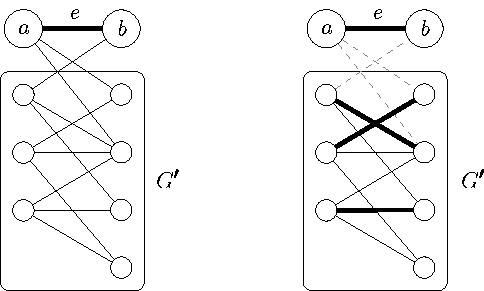
\includegraphics[width=0.5\linewidth]{maxflow/halls-thm-case1.pdf}
        \caption{Case 1. Note that $N(S')$ can have one fewer vertex than $N'(S')$ (this happens when there is an edge from some vertex in $S'$ to $b$, shown as dashed lines). $N(S')$ can also have the same number of vertices as $N'(S')$ if there is no edge going from vertices in $S'$ to $b$. Hence the inequality $|N'(S')| \geq |N(S')|-1$ holds. }
        \label{fig:halls-thm-case1}
    \end{figure}

    Case 2: There exists some $S \subsetneq V_1$ such that $|S| = |N(S)|$. Since $S$ is a proper subset of $V_1$, $|S| < |V_1|$. Let $G_1$ be the subgraph induced by $S \cup N(S)$. $S$ is a proper subset of $V_1$, and $V_1$ satisfies Hall's condition. It follows that any subset of $S$ must also be a subset of $V_1$ and hence satisfies Hall's hypothesis. By induction hypothesis, $G_1$ has a perfect matching $M_1$.

    \begin{figure}[htbp]
        \centering
        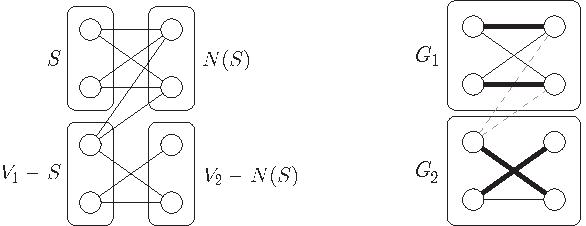
\includegraphics[width=0.6\linewidth]{maxflow/halls-thm-case2.pdf}
        \caption{Case 2. We partition $V_1$ into $S$ and $V_1-S$. The reasoning behind the construction $(S \cup S') \cup (N(S) \cup N(S'))$ when showing that $G_2$ satisfies Hall's condition is that there any neighboring vertices of $S'$ in $G$ not included in $N_{G_2}(S')$ should be included in $N(S)$, which allows us to derive a contradiction if $G_2$ does not satisfy Hall's condition.}
        \label{fig:halls-thm-case2}
    \end{figure}

    Let $G_2$ be the subgraph induced by $(V_1 - S) \cup (V_2 - N(S))$. We claim that $G_2$ also has a perfect matching. It suffices to show that $G_2$ satisfies Hall's condition. Suppose not, then there exists some $S' \subseteq (V_1-S)$ such that $|S'| > |N_{G_2}(S')|$ where $N_{G_2}(S')$ denotes the neighborhood of $S'$ in the subgraph $G_2$. More precisely, $N_{G_2}(S') = N(S) \cap (V_2-N(S))$. Consider the subgraph induced by $(S \cup S') \cup (N(S) \cup N(S'))$. Since $S \cup S'$ is a subset of $V_1$ and $G$ satisfies Hall's condition
    $$
    |N(S \cup S')| \geq |S \cup S'|
    $$
    Since $N(S)$ and $N_{G_2}(S')$ are disjoint,
    $$
    \begin{aligned}
        |N(S \cup S')| &= |N(S) \cup N_{G_2}(S')| \\
        &= |N(S)| + |N_{G_2}(S')| \\
        &= |S| + |N_{G_2}(S')| \\
        &< |S| + |S'| \\
        &= |S \cup S'|
    \end{aligned}
    $$
    which contradicts the assumption that $G$ satisfies Hall's condition. So, $G_2$ must also satisfy Hall's condition and by induction hypothesis, have a perfect matching $M_2$.

    $M_1$ and $M_2$ are perfect matchings within their individual subgraphs that are disjoint. Taking the union of $M_1$ and $M_2$ yields a perfect matching $M$ in $G$.

    By induction, Hall's theorem holds for bipartite graphs of all sizes.
\end{proof}

\section{Disjoint Paths} \index{disjoint path}

Given a graph (directed or undirected) $G=(V,E)$, two non-adjacent nodes $s$ and $t$, we say two paths $p$ and $p'$ from $s \leadsto t$ is are \textit{\textbf{edge-disjoint}} if the two paths do not share a common edge. The \textit{\textbf{maximum edge-disjoint paths}} problem wants to find the maximum number of edge-disjoint $s \to t$ paths. There is a simlilar but different notion of disjoint paths known as \textit{\textbf{interally disjoint paths}} or \textit{\textbf{vertex disjoint paths}} where instead of defining two paths $p$ and $p'$ as disjoint if they do not share an edge, we say two paths are disjoint only if they don't share a vertex. The problem of finding the maximum-size edge-disjoint paths is often useful in the context of communication networks, where we may want to evaluate the \textit{\textbf{fautlt tolerance}} of a network and ensure that there are sufficiently many edge-disjoint paths between two given nodes in the network.

\textit{\textbf{Menger's theorem}} states that the maximum number of edge-disjoint $s-t$ paths is equal to the minimum number of edges in an $s-t$ cut. We will present the theorem for both edge-disjoint paths and vertex disjoint paths. For the edge-based version, we will present an algorithm using max-flow to find the maximum number of edge-disjoint paths, and Menger's theorem follows immediately from the algorithmic construction and the max flow-min cut theorem.

For the vertex-based version, however, things are a little bit more complicated. It is easy to show the vertex-based version of Menger's theorem on a directed graph since we can follow the same construction as in the edge-based version. For undirected graphs, simply making every undirected edge a bidirectional directed edge is not enough, and we need some additional modifications to the original construction. We will also see another not quite constructive proof of Menger's theorem that does not directly rely on the max flow-min cut theorem.

\begin{theorem}[Menger's Theorem (vertex)] \index{Menger's theorem}
    Let $G=(V,E)$ be a graph and let $a,b \in V$ be two \textbf{non-adjacent} distinct vertices. The minimum number of \textbf{vertices} in a $a,b$ separating cut equals the maximum number of \textbf{internally vertex disjoint} $a \leadsto b$ paths in $G$.
\end{theorem}

\begin{theorem}[Menger's Theorem (edge)]
    Let $G=(V,E)$ be a graph and let $a,b \in V$ be two distinct vertices. The minimum number of \textbf{edges} in a $a,b$ separating cut equals the maximum number of \textbf{pairwise edge disjoint} $a \leadsto b$ paths in $G$.
\end{theorem}

\subsection{Edge-Disjoint Paths}

\subsection{Vertex-Disjoint Paths}

\begin{figure}[htbp]
    \centering
    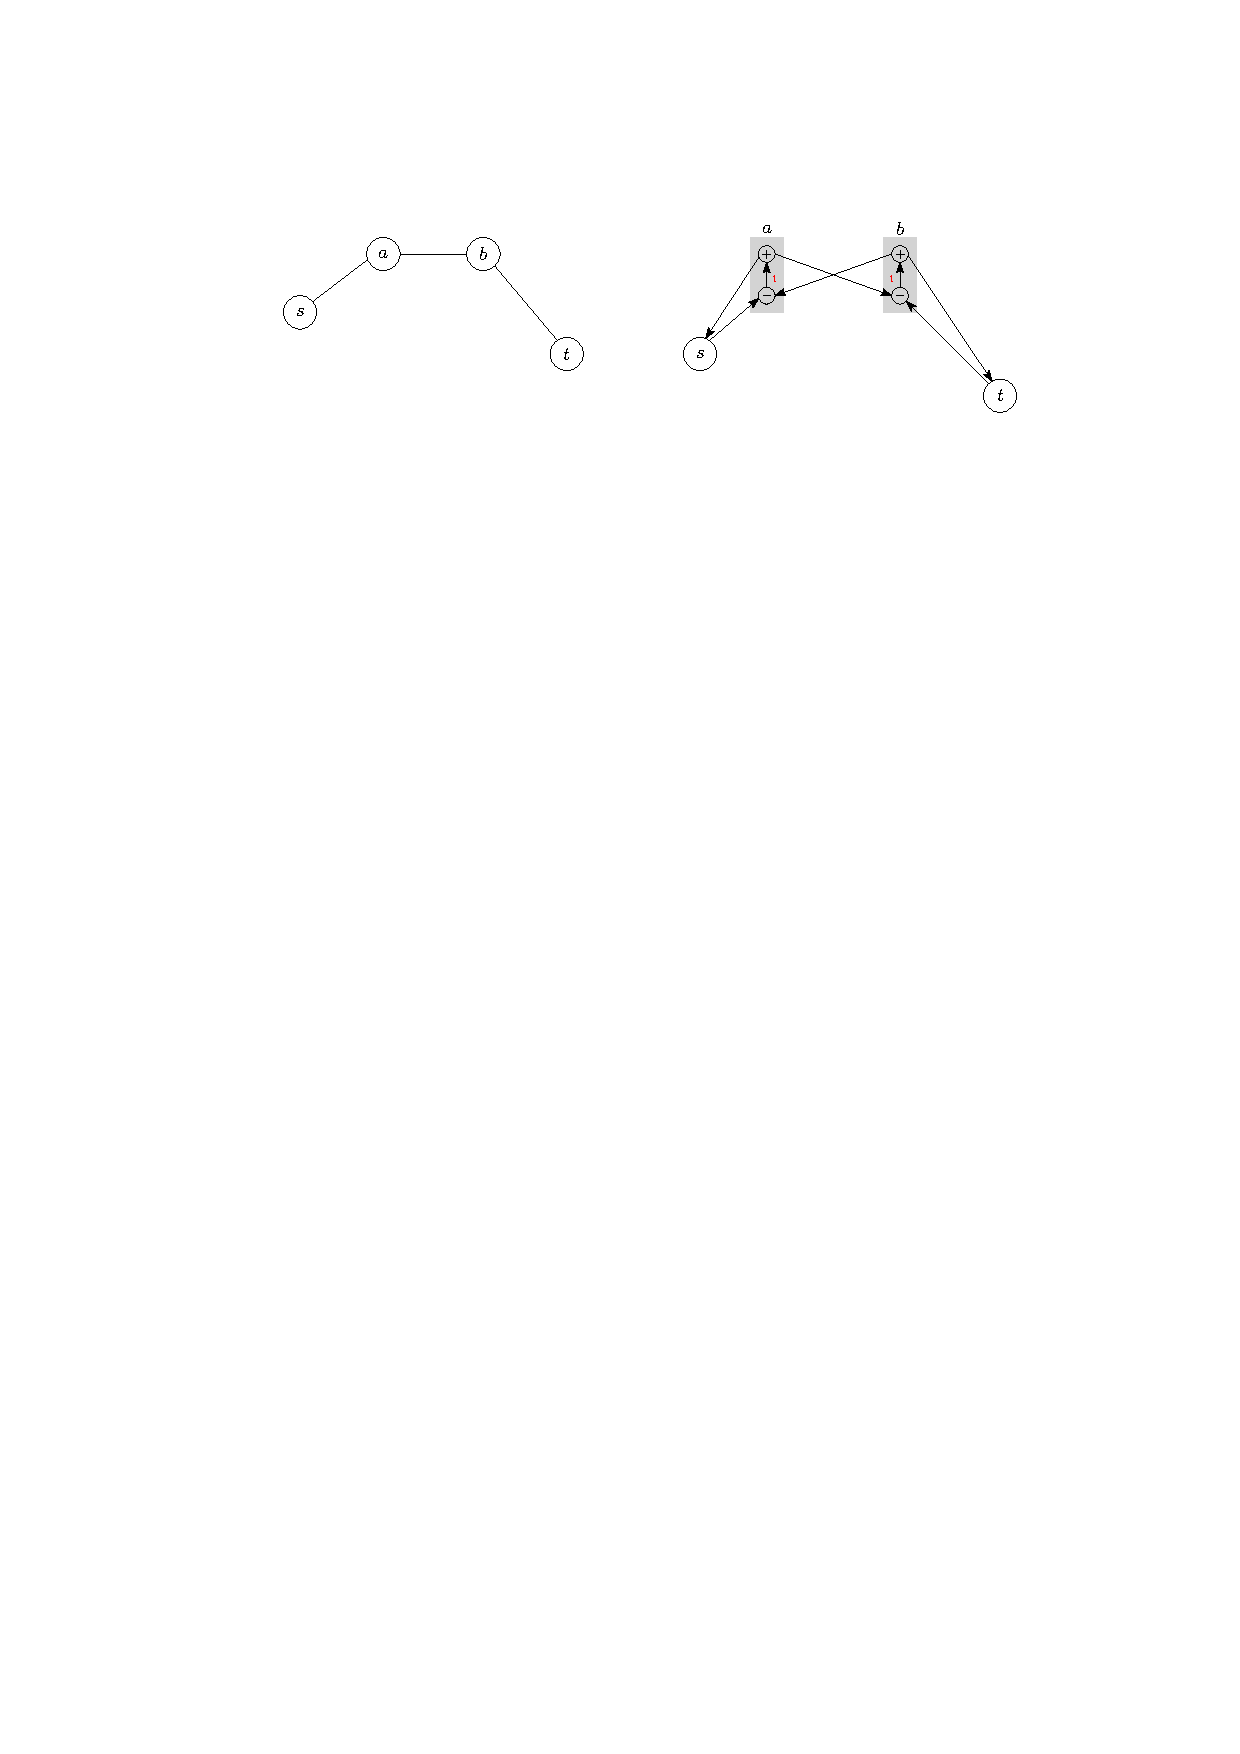
\includegraphics[width=0.9\linewidth]{maxflow/menger-undirected-construct.pdf}
    \caption{The construction converting an undirected graph to a directed graph when finding the maximum number of vertex disjoint paths on an undirected graph. The edges added between the vertices labeled $+$ and $-$ have capacity of 1, and were added to ensure every vertex can only be visited once because as soon as a vertex is visited, the edge become saturated and cannot admit more flow.}
    \label{fig:menger-undirected-construct}
\end{figure}

\begin{figure}[htbp]
    \centering
    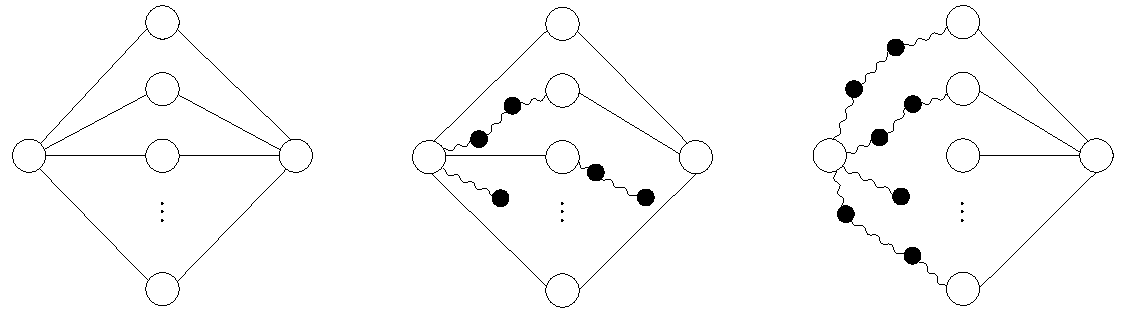
\includegraphics[width=0.9\linewidth]{maxflow/menger-1.pdf}
    \caption{The three possible cases in the inductive proof of Menger's theorem (vertex version). Straight lines indicate an edge connecting two vertices, and squiggly lines denote a path containing at least 3 vertices (including the initial and terminal vertices).}
    \label{fig:menger-undirected-1}
\end{figure}

\chapter{Push-Relabel Algorithm}
\input{notes/pushrelabel.tex}

\part{Complexity}

\part{Linear Programming}

\chapter{Linear Programming}
\section{Linear Programming Optimization}

Linear programming is a commonly used techniques in optimization. In linear programming, we want to optimize (maximize or minimize) a linear function, subject to a set of linear inequalities (called linear constraints). 

\begin{definition}[Linear Constraint] \index{linear function} \index{linear equality} \index{linear inequality} \index{linear constraint}
    Given a set of real numbers $a_1,a_2,\ldots,a_n$ and a set of variables $x_1,x_2,\ldots,x_n$, a \textbf{linear function} $f$ on those variables is
    $$
    f(x_1,\ldots,x_n) = a_1x_1 + a_2x_2 + \cdots + a_nx_n = \sum_{j=1}^n a_jx_j
    $$
    If $b$ is a real number and $f$ is a linear function, then $f(x_1,\ldots,x_n) = b$ is a linear equality ,and $(x_1,\ldots,x_n) \leq b$ and $(x_1,\ldots,x_n) \geq b$ are linear inequalities. Both linear equalities and linear inequalities are called \textbf{linear constraints}.
\end{definition}

Geometrically, a linear function forms a line in $\R^n$. A linear inequality forms a half-space in $\R^n$. All possible solutions to a linear program lies in a convex region called the \textbf{feasible region}. If no such region exsits (no solution satisfies all the contraints), we say the optimization problem is \textbf{infeasible}. The function we wish to optimize is called the \textbf{objective function}, and the value of the objective function evaluated at a particular point is called the \textbf{objective value} at that point. The goal of the linear programming problem is to find a feasible solution that maximizes/minimizes the objective value.

\begin{theorem}[Feasible Region for Linear Programming is Convex]
    Let $\mathbf{x}_1,\mathbf{x}_2 \in \R^n$ be two feasible solutions to the linear programming problem, satisfying some particular constraints. Then, for all $\lambda \in [0,1]$, $\lambda\mathbf{x}_1 + (1-\lambda)\mathbf{x}_2$ is also a solution that satisfies the same constraints.
\end{theorem}

\begin{proof}
    Without loss of generality, suppose that the constraints are given as a system of linear equations $\mathbf{A}\mathbf{x} = \mathbf{b}$. Let $\lambda \in [0,1]$ be arbitrary.
    $$
    \begin{aligned}
        \mathbf{A}(\lambda\mathbf{x}_1 + (1-\lambda)\mathbf{x}_2) &= \lambda\mathbf{A}\mathbf{x}_1 + \mathbf{A}\mathbf{x}_2 - \lambda\mathbf{A}\mathbf{x}_2 \\
        &= \lambda \mathbf{b} + \mathbf{b} - \lambda \mathbf{b} \\
        &= \mathbf{b}
    \end{aligned}
    $$
    Hence, $\lambda\mathbf{x}_1 + (1-\lambda)\mathbf{x}_2$ is also a solution to the system of linear equation and thus is a feasible solution.
\end{proof}

Figure \ref{fig:lp-feasible-region} shows a geometric representation of a linear programming problem with the objective function $x_1+x_2$.

\begin{figure}[htbp]
    \centering
    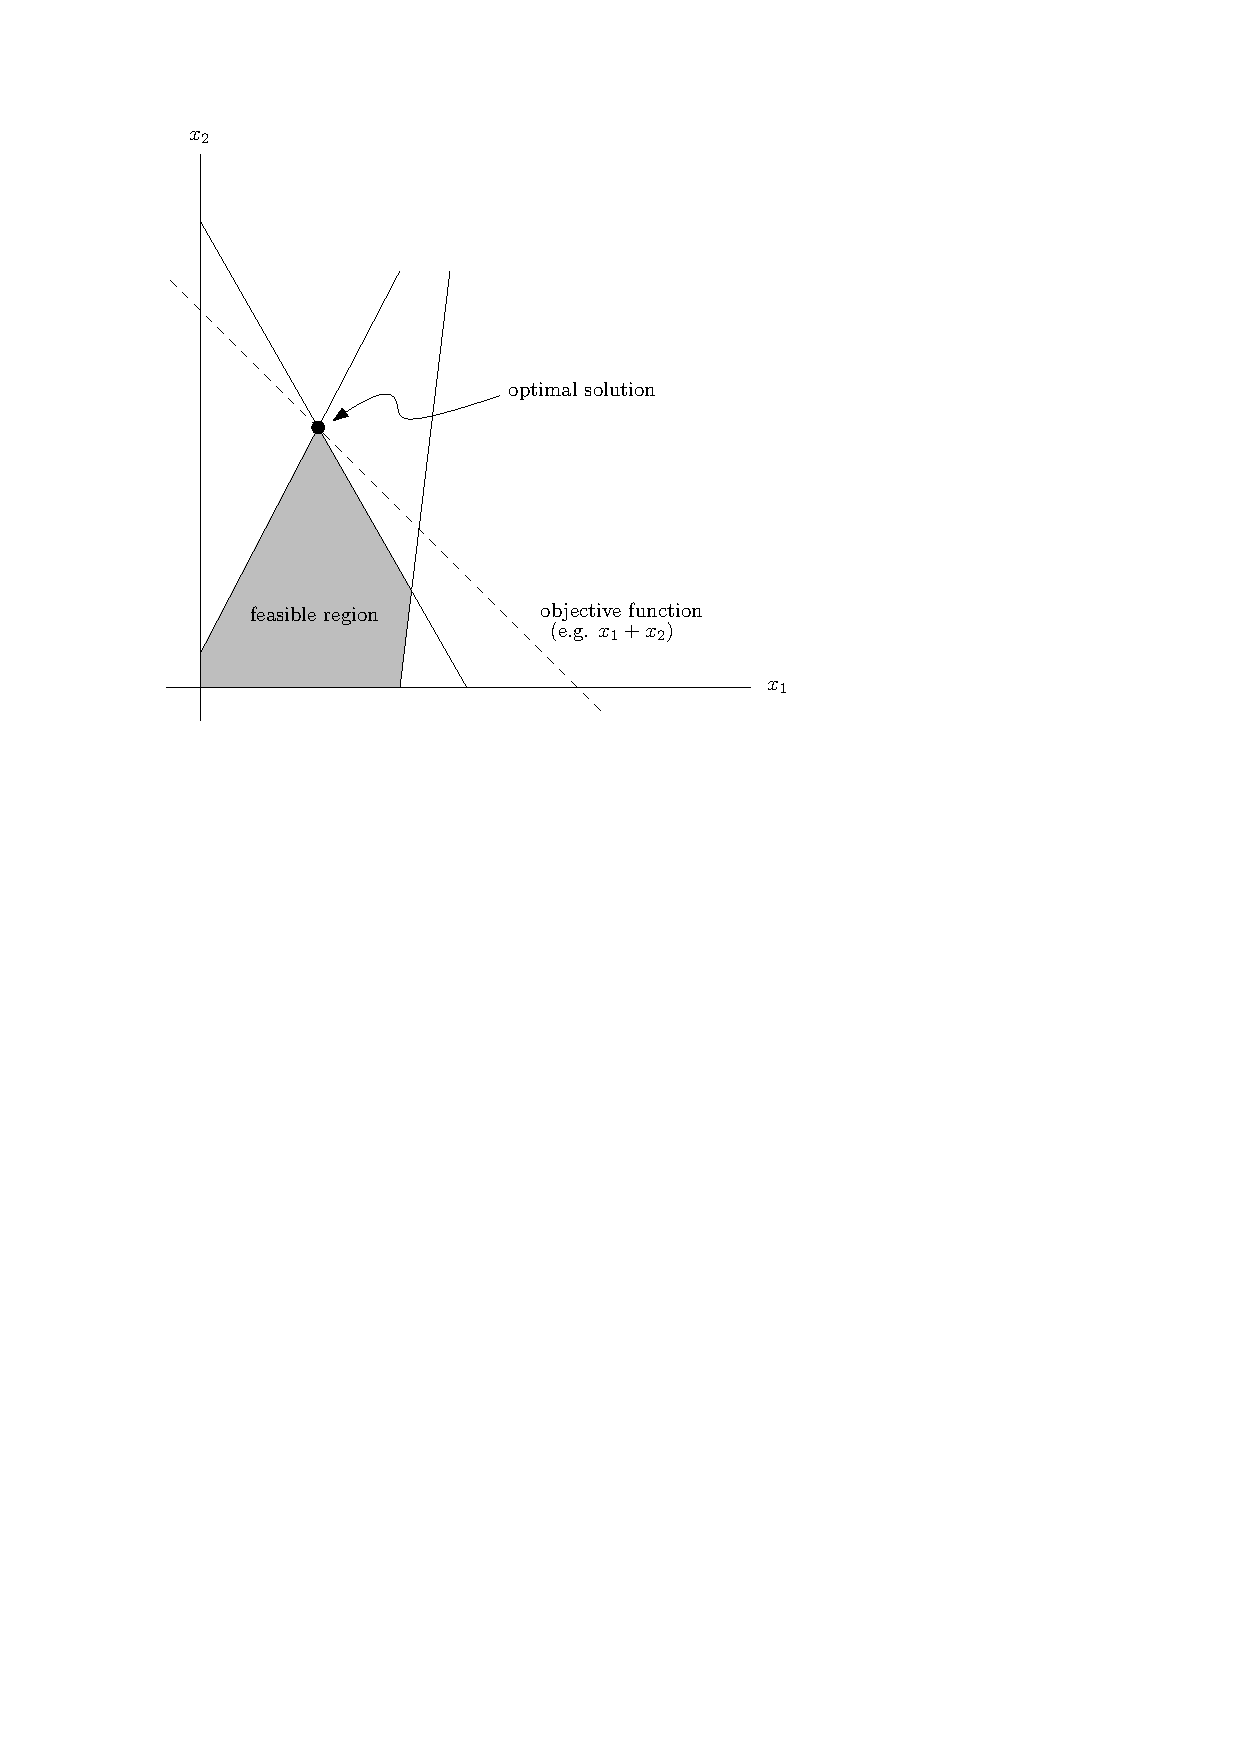
\includegraphics[width=0.6\linewidth]{lp/lp-feasible-region.pdf}
    \caption{A linear programming problem with 2 variables, 4 linear constraints (solid lines), and objective function $x_1+x_2$ (dashed line).}
    \label{fig:lp-feasible-region}
\end{figure}

\section{Standard and Slack Forms}

\subsection{Standard Form}

In standard form, we are given $n$ real numbers $c_1,\ldots,c_n$, $m$ real numbers $b_1,\ldots,b_m$, and $mn$ real numbers $a_{ij}$ for $i \in \{1,\ldots,m\}$ and $j \in \{1,\ldots,n\}$. We wish to

Maximize $\displaystyle \sum_{j=1}^n c_j x_j$ \\
Subject to
\[
    \begin{aligned}
        \sum_{j=1}^n a_{ij} x_j &\leq b_1 & \text{for $i = 1,\ldots,m$} \\
        x_j &\geq 0 & \text{for $j = 1,\ldots,n$}
    \end{aligned}
\]

or, equivalently, in vectorized form

Maximize $\mathbf{c}^\top \mathbf{x}$ \\
Subject to $\mathbf{A}\mathbf{x} \leq \mathbf{b}$ and $\mathbf{x} \geq \boldsymbol{0}$,

where $\mathbf{c}$ is an $n$-vector, $\mathbf{x}$ is an $n$-vector, $\mathbf{b}$ is an $m$-vector, and $\mathbf{A}$ is an $m \times n$ matrix. This can also be written in as a tuple $(\mathbf{A},\mathbf{b},\mathbf{c})$ as a shorthand.

This vectorized form is often used in machine learning because vectorized operations can be carried out more quickly using the GPU.

\subsection{Conversion From Non-standard Form to Standard Form}

A linear programming problem might not be in standard form, but it is easy to convert from non-standard form to standard form.

If \begin{itemize}
    \item the objective is minimization rather than maximization $\Rightarrow$ flip the sign of coefficients;
    \item there are variables without nonnegativity constraints $\Rightarrow$ say a variable $x_j$ does not have  nonnegativity constraints, replace $x_j$ with $x_j' - x_j''$ and add constraints $x_j' \geq 0$ and $x_j'' \geq 0$;
    \item the constraints are equality constraints rather than $\leq$ $\Rightarrow$ replace the constraint with two non-strict inequality constraints ($\leq$ and $\geq$);
    \item the constraints are in the opposite direction ($\geq$ instead of $\leq$) $\Rightarrow$ multiply both sides by -1 
\end{itemize}

\subsection{Slack Form}

Maximize $\displaystyle z = v + \sum_{j=1}^n c_j x_j$ \\
Subject to
\[
    \begin{aligned}
        s_i &= b_1 - \sum_{j=1}^n a_{ij} x_j & \text{for $i = 1,\ldots,m$} \\
        x_j,s_i &\geq 0 & \text{for $j = 1,\ldots,n$ and $i = 1,\ldots,m$ }
    \end{aligned}
\]

or, equivalently, in vectorized form

Maximize $z = v + \mathbf{c}^\top \mathbf{x}$ \\
Subject to $\mathbf{s} = \mathbf{b} - \mathbf{A}\mathbf{x}$ and $\mathbf{x},\mathbf{s} \geq \boldsymbol{0}$.

We call the variables on the left-hand side of the equality constraints the \textbf{basic variables}, and the ones on the right-hand side the \textbf{non-basic variables}.

Similarly, a slack from can be concisely defined by a tuple $(N,B,\mathbf{A},\mathbf{b},\mathbf{c},v)$, where $N$ is the set of indices of the non-basic variables, $B$ is the set of indices of the basic variables such that $|N| = n$, $|B|=m$ and $N \cup B = \{1,2,\ldots,n+m\}$.

It is called the slack from because the variable $s_i$ (or in vectorized form $\mathbf{s}$) measures remaining ``slack'' or difference between two sides of the original inequality constraints. This is related to the simplex algorithm where we increase the non-basic variables as much as possible until we hit a bottleneck -- having no more slack for that non-basic variable.

\section{Geometry of Linear Programming}

Consider the following system of inequalities
$$
\begin{aligned}
    x_1 + x_2 + x_3 &\leq 1 \\
    x_1,x_2,x_3 &\geq 0
\end{aligned}
$$
This is the type of inequalities that we often encounter in linear programming problems. The points that satisfy these inequalities forms a 3D polytope.

\begin{figure}[htbp]
    \centering
    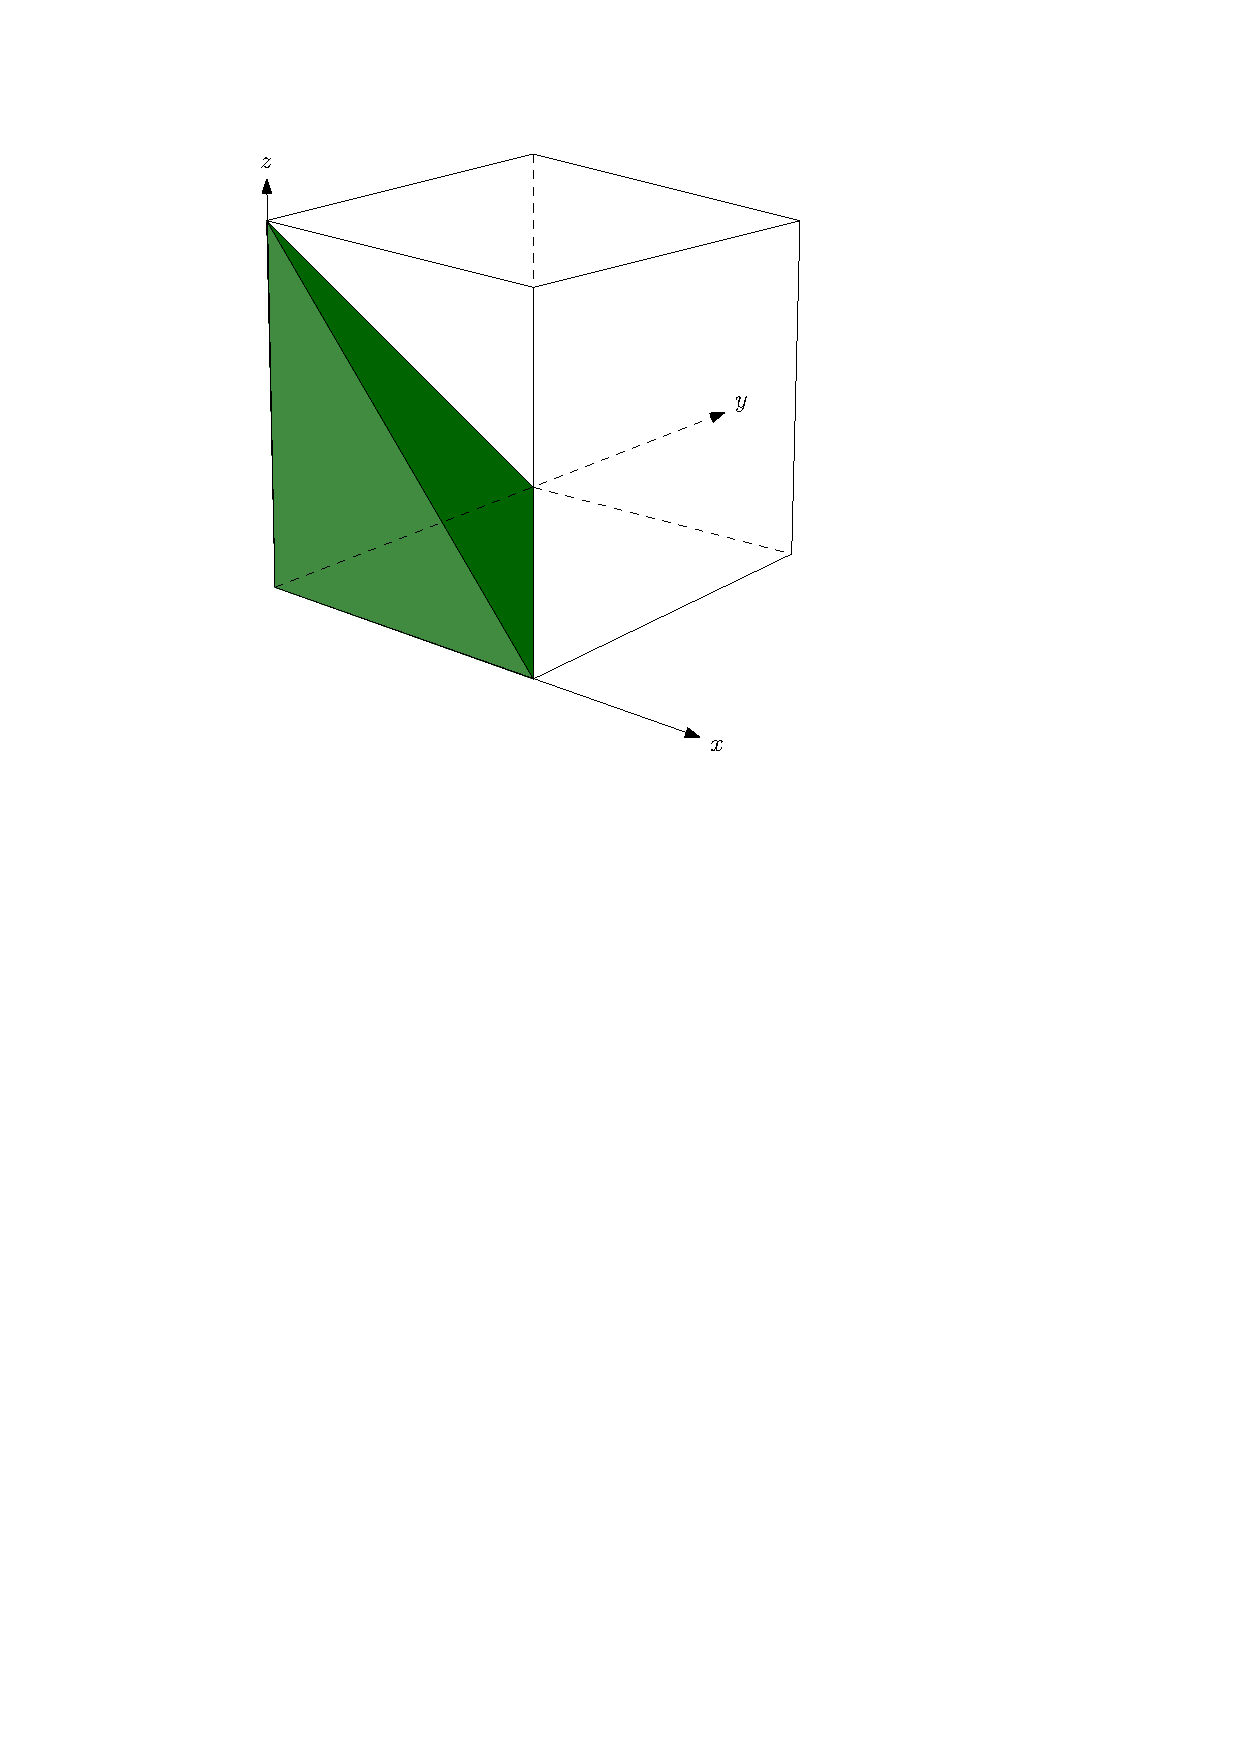
\includegraphics[width=0.4\linewidth]{lp/3d-polytope.pdf}
    \caption{A 3D polytope.}
    \label{fig:3d-polytope}
\end{figure}

\subsection{Hyperplane and Halfspace} \index{hyperplane} \index{halfspace} \index{supporting hyperplane}
In general, the set $\{ x \in \R^n \mid a^\top x = b \}$ is called a hyperplane. For all lines in the \textbf{hyperplane} $H = \{ x \in \R^n \mid a^\top = b \}$ that intersects the line $\ell = \{ta \mid t \in \R\}$, the line is also perpendicular to $\ell$. As a simple example, consider the two-dimensional case where $a = [1\;\;-1]^\top$.

The set $\{ \mathbf{x} \in \R^n \mid \mathbf{a}^\top \mathbf{x} \leq b \}$ is called a \textbf{halfspace}, and $\{ \mathbf{x} \in \R^n \mid \mathbf{a}^\top \mathbf{x} = b \}$ is called the \textbf{supporting hyperplane}.

\subsection{Polyhedron and Polytope} \index{polyhedron} \index{polytope} \index{face} \index{facet}

A set that is the intersection of halfspaces is called a \textbf{polyhedron}. A polyhedron can be defined as $\{x \in \R^n \mid \mathbf{A}\mathbf{x} \leq \mathbf{b} \}$ for some matrix $\mathbf{A}$ and vector $\mathbf{b}$.

A polyhedron $P \subseteq \R^n$ is unbounded if there exists a point $\mathbf{x} \in P$ and a direction $\mathbf{v} \in \R^n$ such that for every $t \geq 0$, $\mathbf{x} + t \mathbf{v} \in P$. If a polyhedron is bounded, we call it a \textbf{polytope}.

A \textbf{face} of a polyhedron $P = \{\mathbf{x} \in \R^n \mid \mathbf{A}\mathbf{x} \leq \mathbf{b} \}$ is a set $F = \{ \mathbf{x} \in \R^n \mid \mathbf{A}\mathbf{x} \leq b \} \cap \{ \mathbf{x} \in \R^n \mid \forall i \in S.\, \mathbf{a}_i \mathbf{x} = \mathbf{b}_i \}$ where $\mathbf{a}_i$ is a row vector denoting the $i$th row of matrix $\mathbf{A}$, and $S$ is some subset of the rows of $\mathbf{A}$. Intuitively, a face of a polyhedron is just one of its surface.

Assuming that $F \neq \emptyset$, we define $S_F$ to be the set of all $i \in S$ such that $\mathbf{a}_i \mathbf{x} = \mathbf{b}_i$ for all $\mathbf{x} \in F$ (we can intutively think this as the rows of constraints that created the face $F$). Let $\mathbf{A}_F$ be the submatrix of $\mathbf{A}$ containing rows of $A$ indexed by $S_F$. If the rank of $\mathbf{A}_F$ is $n-j$, we say $F$ is a face of \textbf{dimension} $j$, or a $j$-face. The dimension of a polytope can be defined similarly. Faces of dimension one lower than the dimension of $P$ are called \textbf{facets}, faces of dimension 1 are called \textbf{edges}, faces of dimension 0 are called \textbf{vertices}.

\subsection{Convex Hull}

A polytope can be determined by its vertices.

\begin{definition}[Convex Hull] \index{convex hull}
    The convex hull of the points $\mathbf{v}_1,\ldots,\mathbf{v}_n \in \R^n$ is defined as the set
    $$
    \mathrm{conv} \{\mathbf{v}_1,\ldots,\mathbf{v}_n\} = \{ \lambda_1 \mathbf{v}_1 + \cdots + \lambda_n \mathbf{v}_n \mid \forall i \in \{1,\ldots,n\}.\, \lambda_i \geq 0,\; \lambda_1+\cdots+\lambda_n = 1 \}
    $$
\end{definition}

\begin{theorem} \label{thm:convex-hull-polytope}
    A polytope $P$ with vertices $\mathbf{v}_1 \ldots \mathbf{v}_n$ is equal to the convex hull of the vertices.
    $$
    P = \mathrm{conv} \{\mathbf{v}_1,\ldots,\mathbf{v}_n\}
    $$
\end{theorem}

\begin{proof}
    TODO. (by showing $\mathrm{conv} \{\mathbf{v}_1,\ldots,\mathbf{v}_n\} \subseteq P$ and $P \subseteq \mathrm{conv} \{\mathbf{v}_1,\ldots,\mathbf{v}_n\}$)
\end{proof}

An important implication of Theorem \ref{thm:convex-hull-polytope} is that we can always find an optimal solution to a linear program at a vertex of the feasible region. This will become the basis of the simplex algorithm in the coming chapter.

\begin{theorem}[Foundamental Theorem of Linear Programming]
    If $\max \{ \mathbf{c}^\top \mathbf{x} \in \R \mid \mathbf{A}\mathbf{x} \leq \mathbf{b},\, \mathbf{x} \geq \textbf{0} \}$ is a linear program whose feasible region $\{ \mathbf{x} \in \R^n \mid \mathbf{A}\mathbf{x} \leq \mathbf{b},\, \mathbf{x} \geq \textbf{0} \}$ is a polytope, then the linear program has an optimal solution at a vertex of $P$.
\end{theorem}

\begin{proof}
    Let $\mathbf{x}$ be an optimal solution to the linear program. By Theorem \ref{thm:convex-hull-polytope}, $\mathbf{x}$ can be expressed as a convex combination.
    $$
    \lambda_1 \mathbf{v}_1 + \cdots + \lambda_n \mathbf{v}_n \quad \forall i \in \{1,\ldots,n\}.\, \lambda_i \geq 0,\; \lambda_1+\cdots+\lambda_n = 1
    $$
    where $\mathbf{v}_1,\ldots,\mathbf{v}_n$ are the vertices of $P$. It follows by substitution that
    $$
    \mathbf{c}^\top \mathbf{x} = \mathbf{c}^\top \lambda_1 \mathbf{v}_1 + \cdots + \mathbf{c}^\top \lambda_n \mathbf{v}_n \leq  \lambda_1 \max_{i=1}^n (\mathbf{c}^\top \mathbf{v}_i) + \cdots + \lambda_n \max_{i=1}^n (\mathbf{c}^\top \mathbf{v}_i) = \max_{i=1}^n (\mathbf{c}^\top \mathbf{v}_i)
    $$
    Therefore, a maximum of $\mathbf{c}^\top \mathbf{v}_i$ is also a maximum of $\mathbf{c}^\top \mathbf{x}$.
\end{proof}

\chapter{Simplex Algorithm for LP}
\section{Geometric Intuition}

The geometry behind the simplex algorithm is actually quite intuitive, especially after we have proved that there is always at least one optimal solution lying on a vertex of the feasible region. The simplex algorithm starts at an initial vertex, follows the edges of the polytope to neighboring vertices, and checks each vertices along the way. The algorithm terminates when the objective function cannot be improved anymore.

\begin{figure}[htbp]
    \centering
    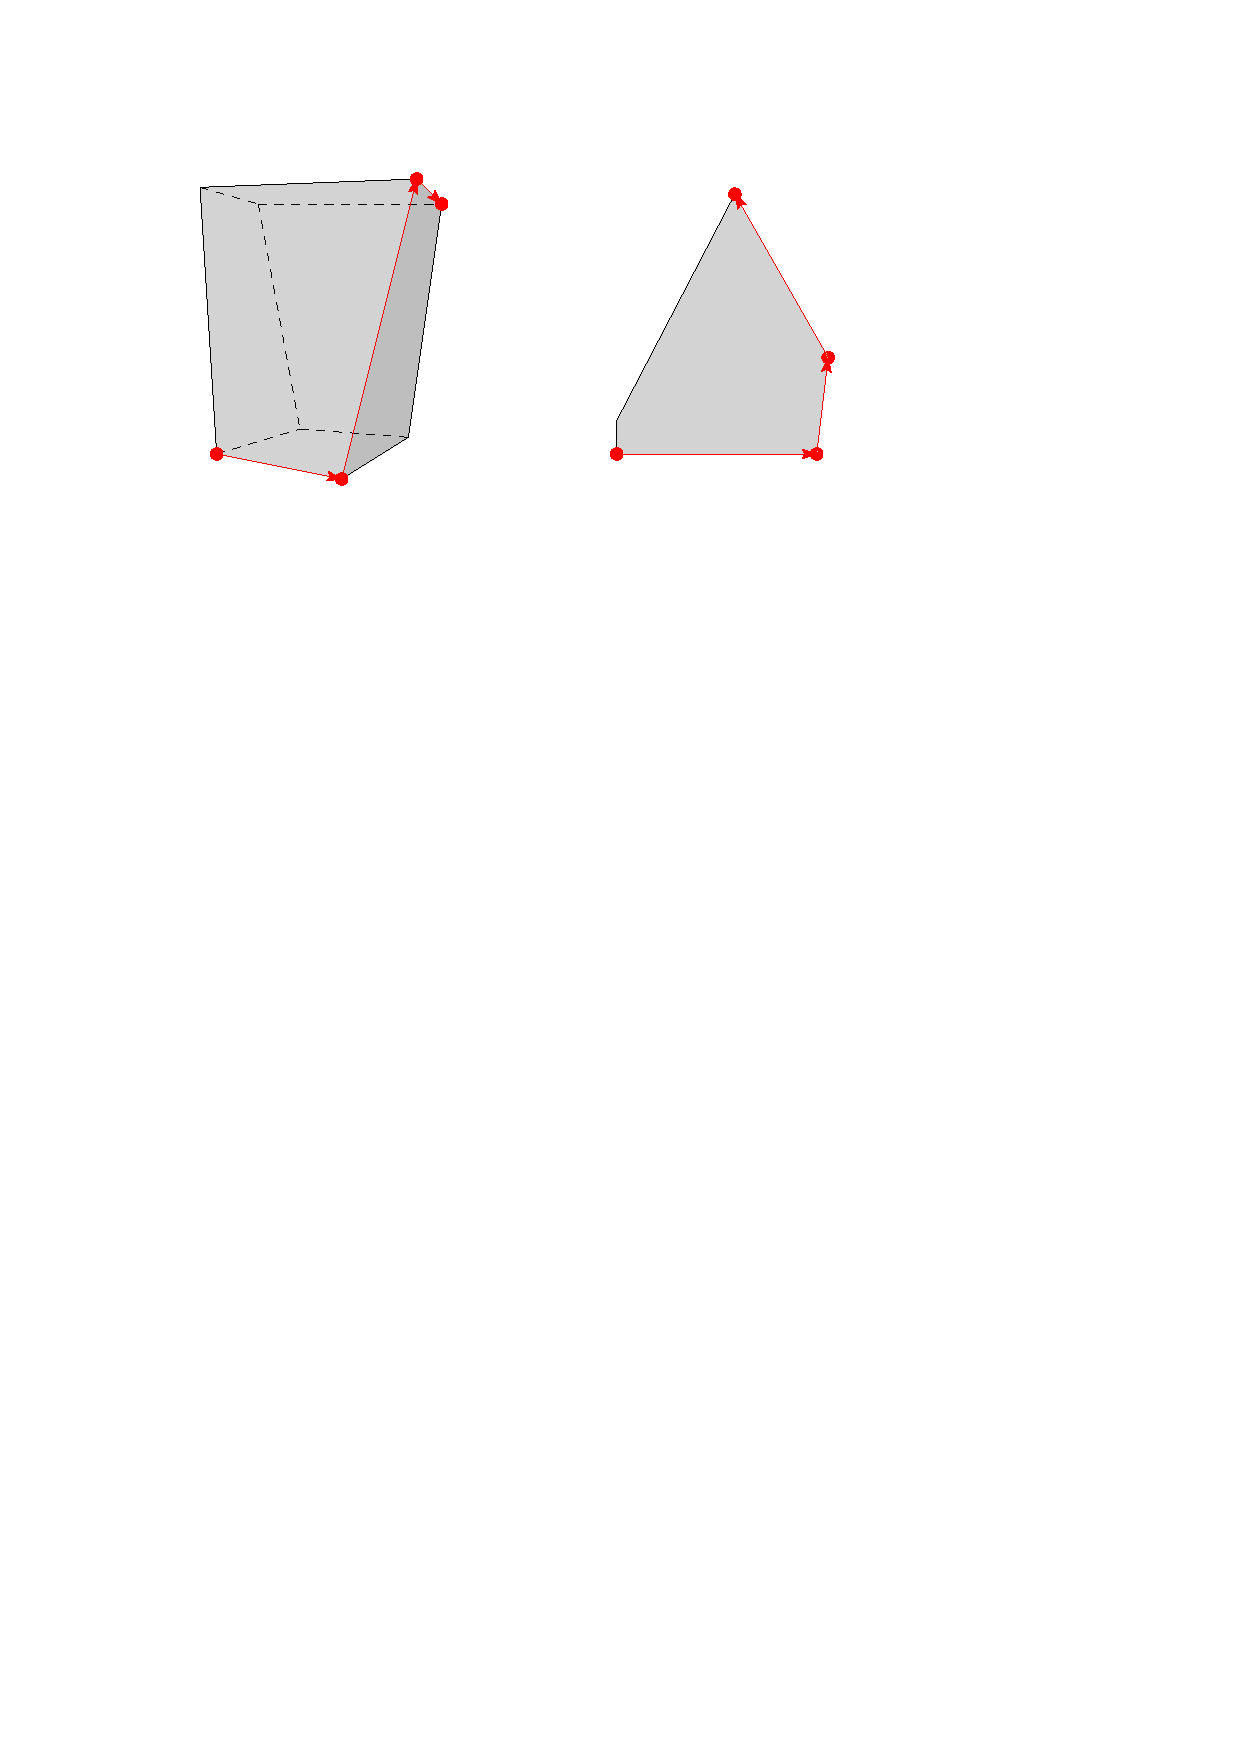
\includegraphics[width=0.5\linewidth]{lp/simplex-geometric-2.pdf}
    \caption{The geometric intuition behinds the simplex algorithm. The figure shows the simplex algorithm trying to find the optima on a 3-dimensional and 2-dimensional polytope.}
    \label{fig:simplex-geometric}
\end{figure}

\section{Pivoting}

The way the simplex algorithm navigates through the polytope and jumps between vertices in through an operation called \textit{\textbf{pivoting}}.

During pivoting, we select a non-basic variable $x_e$ as the \textit{\textbf{entering variable}}, and a basic variable $x_l$ as the \textit{\textbf{leaving variable}}. The pivot operation switches the roles of the entering and leaving variable. $x_e$ becomes a new basic variable, and $x_l$ becomes a non-basic variable. Because of this, we also need to update the expression of other basic variables as well as the objective function. Geometrically, this corresponds to following an edge of the feasible to a neighboring vertex.

Pivoting not only affects the entering and leaving variables. Because it changes the roles of the variables, we need to update the entire linear program so that $x_e$ no longer appears as a non-basic variable in any expressions. Similarly, we also want $x_l$ to appear as a non-basic variable in every expressions. Such updates also need to be applied to the objective function.

\subsection{Update Coefficient Matrix for the Entering Variable}

Suppose we have selected $x_e$ as the entering variable and $x_l$ as the leaving variable. Currently, $x_e$ is a non-basic variable, and $x_l$ is a basic variable where
$$
x_l = b_l - a_{l1}x_1 - \cdots - a_{lj}x_j - a_{le}x_e
$$
Move the entering variable to the left-hand side and move the leaving variable to the right-hand side.
$$
a_{le}x_e = b_l - a_{l1}x_1 - \cdots - a_{lj}x_j - x_l
$$
Divide both sides by $a_{le}$, the coefficient of the entering variable.
$$
x_e = \frac{b_l}{a_{le}} - \frac{a_{l1}}{a_{le}}x_1 - \cdots - \frac{a_{lj}}{a_{le}}x_j - \frac{1}{a_{le}}x_l
$$
Now, $x_e$ has become a basic variable, and $x_l$ has become a non-basic variable.

\subsection{Update Coefficient Matrix for Other Basic Variables}

Since we have made $x_e$ a basic variable, expressed in terms of the non-basic variables, we need to update the expressions of the remaining basic variables to reflect this change.

Consider the $i$th basic variable $x_i$, with the expression
$$
x_i = b_1 - a_{i1}x_1 - \cdots - a_{ij}x_j - a_{ie}x_e
$$
We can substitute $x_e$ with its new expression in terms of the non-basic variables
$$
x_i = b_1 - a_{i1}x_1 - \cdots - a_{ij}x_j - a_{ie}\left( \frac{b_l}{a_{le}} - \frac{a_{l1}}{a_{le}}x_1 - \cdots - \frac{a_{lj}}{a_{le}}x_j - \frac{1}{a_{le}}x_l \right) 
$$
Combine like terms.
$$
x_i = \left( b_i - a_{ie}\frac{b_l}{a_{le}} \right) - \left( a_{i1}-a_{ie}\frac{a_{l1}}{a_{le}} \right) x_1 - \cdots - \left( a_{ij}-a_{ie}\frac{a_{lj}}{a_{le}} \right) x_j - \left( -a_{ie}\frac{1}{a_{le}} \right) x_l
$$

\subsection{Update Objective Function}

The objective function
$$
z = v + \sum_{j=1}^n c_j x_j
$$
also needs to be updated.

In particular, we will substitute $x_e$ with its new expression in terms of the non-basic variables. This is similar to how we update the basic variables.
$$
z = v + c_1x_1 + \cdots + c_j x_j + c_e \left( \frac{b_l}{a_{le}} - \frac{a_{l1}}{a_{le}}x_1 - \cdots - \frac{a_{lj}}{a_{le}}x_j - \frac{1}{a_{le}}x_l \right)
$$
Again, we combine like terms, yielding
$$
z = \left( v + c_e \frac{b_l}{a_{le}} \right) + \cdots + \left( c_j - c_e \frac{a_{lj}}{a_{le}} \right) x_j + \left( - c_e \frac{1}{a_{le}} \right)x_l
$$

\subsection{Pivoting Algorithm}

Based on our derivation above, we can implement the pivot operation as follows. The procedure \proc{Pivot} takes in the tuple $(N,B,A,b,c,v)$ representing a linear program in slack form, along with the index of the leaving and entering variables $l$ and $e$, and outputs a new tuple $(\hat{N},\hat{B},\hat{A},\hat{b},\hat{c},\hat{v})$.

Recall that $N$ is the set of indices of the non-basic variables, $B$ is the set of indices of the basic variables, $A$ is the coefficient matrix, $b$ and $c$ are column vectors. In the algorithm, we assume we can access the $i,j$-entry of a matrix $A$ using $a_{ij}$ representing the linear program after pivoting.

\begin{codebox}
    \Procname{$\proc{Pivot}(N,B,A,b,c,v,l,e)$}
    \li \Comment{Initialize $m \times n$ matrix}
    \li $\hat{A} = [[]]$
    \li \Comment{Calculate coefficients for new basic variable $x_e$}
    \li $\hat{b}_e = b_l/a_{le}$
    \li \For $j \in N - \{e\}$ \Do
        \li $\hat{a}_{ej} = a_{lj}/a_{le}$
    \End
    \li $\hat{a}_{el} = 1/a_{le}$
    \li \Comment{Calculate coefficients for the remaining constraints}
    \li \For $i \in B - \{l\}$ \Do
        \li $\hat{b}_i = b_i - a_{ie} \hat{b}_e$
        \li \For $j \in N - \{e\}$ \Do
            \li $\hat{a}_{ij} = a_{ij} - a_{ie} \hat{a}_{ej}$
        \End
        \li $\hat{a}_{il} = -a_{ie} \hat{a}_{el}$
    \End
    \li \Comment{Calculate the new objective function}
    \li $\hat{v} = v + c_e \hat{b}_e$
    \li \For $j \in N - \{e\}$ \Do
        \li $\hat{c}_j = c_j - c_e \hat{a}_{ej}$
    \End
    \li $\hat{c}_l = -c_e \hat{a}_{el}$
    \li \Comment{Update new sets of basic and non-basic variables}
    \li $\hat{N} = N - \{e\} \cup \{l\}$
    \li $\hat{B} = B - \{l\} \cup \{e\}$ 
    \li \Return $(\hat{N},\hat{B},\hat{A},\hat{b},\hat{c},\hat{v})$ 
\end{codebox}

\section{Simplex Algorithm}

\subsection{Basic Feasible Solution}

The simplex algorithm follows the intuitive that we have developed throughout the chapter. We start from a vertex (say, the origin) keep moving to a neighboring vertex if such move can increase the value of the objective function. We have seen that this can be done through the pivot operation. To make this idea more concrete, let's define a basic solution and a basic feasible solution.

\begin{definition}[Basic Solution] \index{basic solution}
    A solution $\mathbf{x}$ of $\mathbf{A}\mathbf{x} = \mathbf{b}$ is a \textit{\textbf{basic solution}} if the set $\{ \mathbf{a}_i \mid x_i \neq 0 \}$ (the columns of $A$ corresponding to a non-zero variable) is linearly independent. Equivalently, this means that there are $n$ linearly independent constraints.
\end{definition}

\begin{definition}[Basic Feasible Solution] \index{basic feasible solution}
    A basic solution that is also a feasible solution is called a basic feasible solution.
\end{definition}

In slack form, a basic solution can be obtained by setting all non-basic variables to 0.

The goal of the simplex algorithm is to, in each iteration, reformulate the linear program so that the basic solution leads to a greater objective value. This is done by selecting the tightest basic variable as the leaving variable, a non-basic variable whose coefficient in the objective function is positive as the entering variable, and performing the pivot operation.

\subsection{Example of Simplex Algorithm}

As an example, let's examine the linear program on page 865 of CLRS.
\[
    \begin{aligned}
        \text{maximize \quad } & 3x_1 + x_2 + 2x_3 \\
        \text{subject to \quad } &x_1 + x_2 + 3x_3 &\leq 30 \\
        &2x_1 + 2x_2 + 5x_3 &\leq 24 \\
        &4x_1 + x_2 + 2x_3 &\leq 36 \\
        &x_1, x_2, x_3 &\geq 0
    \end{aligned}
\]
Convert it to slack form
\[
    \begin{aligned}
        \text{maximize \quad }  z &= 3x_1 + x_2 + 2x_3 \\
        \text{such that \quad } x_4 &= 30 - x_1 - x_2 - 3x_3 \\
        x_5 &= 24 - 2x_1 - 2x_2 - 5x_3 \\
        x_6 &= 36 - 4x_1 - x_2 - 2x_3 \\
        & x_1, x_2, x_3, x_4, x_5, x_6 \geq 0
    \end{aligned}
\]
Set all non-basic variables $x_1,x_2,x_3$ to 0 and obtain the basic solution $x_1=0,\,x_2=0,\,x_3=0,\,x_4=30,\,x_5=24,\,x_6=36$. The objective value for this basic solution is 0. (Starts from the origin of the feasible region.)

Select $x_1$ as entering variable because it has a positive coefficient in the objective function. The tightest constraint is $x_6$ since $x_1$ can only increase by 9 while maintaining $x_6 \geq 0$. Perform pivot operation, and we get
\[
    \begin{aligned}
        \text{maximize \quad }  z &= 27 + \frac{x_2}{4} + \frac{x_3}{2} - \frac{3x_6}{4} \\
        \text{such that \quad } x_1 &= 9 - \frac{x_2}{4} - \frac{x_3}{2} - \frac{x_6}{4} \\
        x_4 &= 21 - \frac{x_2}{4} - \frac{x_3}{2} - \frac{x_6}{4} \\
        x_5 &= 6 - \frac{3x_2}{2} - 4x_3 + \frac{x_6}{2} \\
        & x_1, x_2, x_3, x_4, x_5, x_6 \geq 0
    \end{aligned}
\]
The basic solution is currently $x_1=9,\,x_2=0,\,x_3=0,\,x_4=21,\,x_5=6,\,x_6=0$ with $z=27$. Select $x_3$ as the next entering variable. $x_5$ has the tightest constraint, so $x_5$ is the leaving variable. Perform pivot operation.
\[
    \begin{aligned}
        \text{maximize \quad }  z &= \frac{111}{4} + \frac{x_2}{16} - \frac{x_5}{8} - \frac{11x_6}{16} \\
        \text{such that \quad } x_1 &= \frac{33}{4} - \frac{x_2}{16} + \frac{x_5}{8} - \frac{5x_6}{16} \\
        x_3 &= \frac{3}{2} - \frac{3x_2}{8} - \frac{x_5}{4} + \frac{x_6}{8} \\
        x_4 &= \frac{69}{4} + \frac{3x_2}{16} - \frac{5x_5}{8} - \frac{x_6}{16} \\
        & x_1, x_2, x_3, x_4, x_5, x_6 \geq 0
    \end{aligned}
\]
The basic solution is currently $x_1=\frac{33}{4},\,x_2=0,\,x_3=\frac{3}{2},\,x_4=\frac{69}{4},\,x_5=0,\,x_6=0$ with $z=\frac{111}{4}$. Select $x_2$ as the next entering variable as it is the only variable with a positive coefficient in the objective function. $x_3$ has the tightest constraint while $x_4$ puts no constraint on how much we can increase $x_2$. $x_3$ will be the next leaving variable.
\[
    \begin{aligned}
        \text{maximize \quad }  z &= 28 - \frac{x_3}{6} - \frac{x_5}{6} - \frac{2x_6}{3} \\
        \text{such that \quad } x_1 &= 8 + \frac{x_3}{6} + \frac{x_5}{6} - \frac{x_6}{3} \\
        x_2 &= 4 - \frac{8x_3}{3} - \frac{2x_5}{3} \frac{x_6}{3} \\
        x_4 &= 18 - \frac{x_3}{2} + \frac{x_5}{2} + 0x_6 \\
        & x_1, x_2, x_3, x_4, x_5, x_6 \geq 0
    \end{aligned}
\]
Observe that at this stage, none of the nonbasic variables in the objective function has positive coefficient, so it cannot be optimized anymore. The optimal solution to the original linear program is $x_1=8,x_2=4,x_3=0$ with $z=28$.

Going back to our geometric intuition for the simplex algorithm, the algorithm can be understood as follows. We start from the origin $(0,0,0)$. Increase $x_1$ until it hits the barrier set forth by $x_6$ (tightest constraint). Increase $x_3$ until it hits the barrier set forth by $x_5$ (tightest constraint). Increase $x_2$ until it hits the barrier by $x_3$ (tightest constraint). Indeed, just as described in our geometric interpretation, the simplex algorithm travels along the edges of the feasible region to neighboring vertices and finds an optimal solution at one of vertices of the feasible region. See Figure \ref{fig:simplex-example}.

\begin{figure}[htbp]
    \centering
    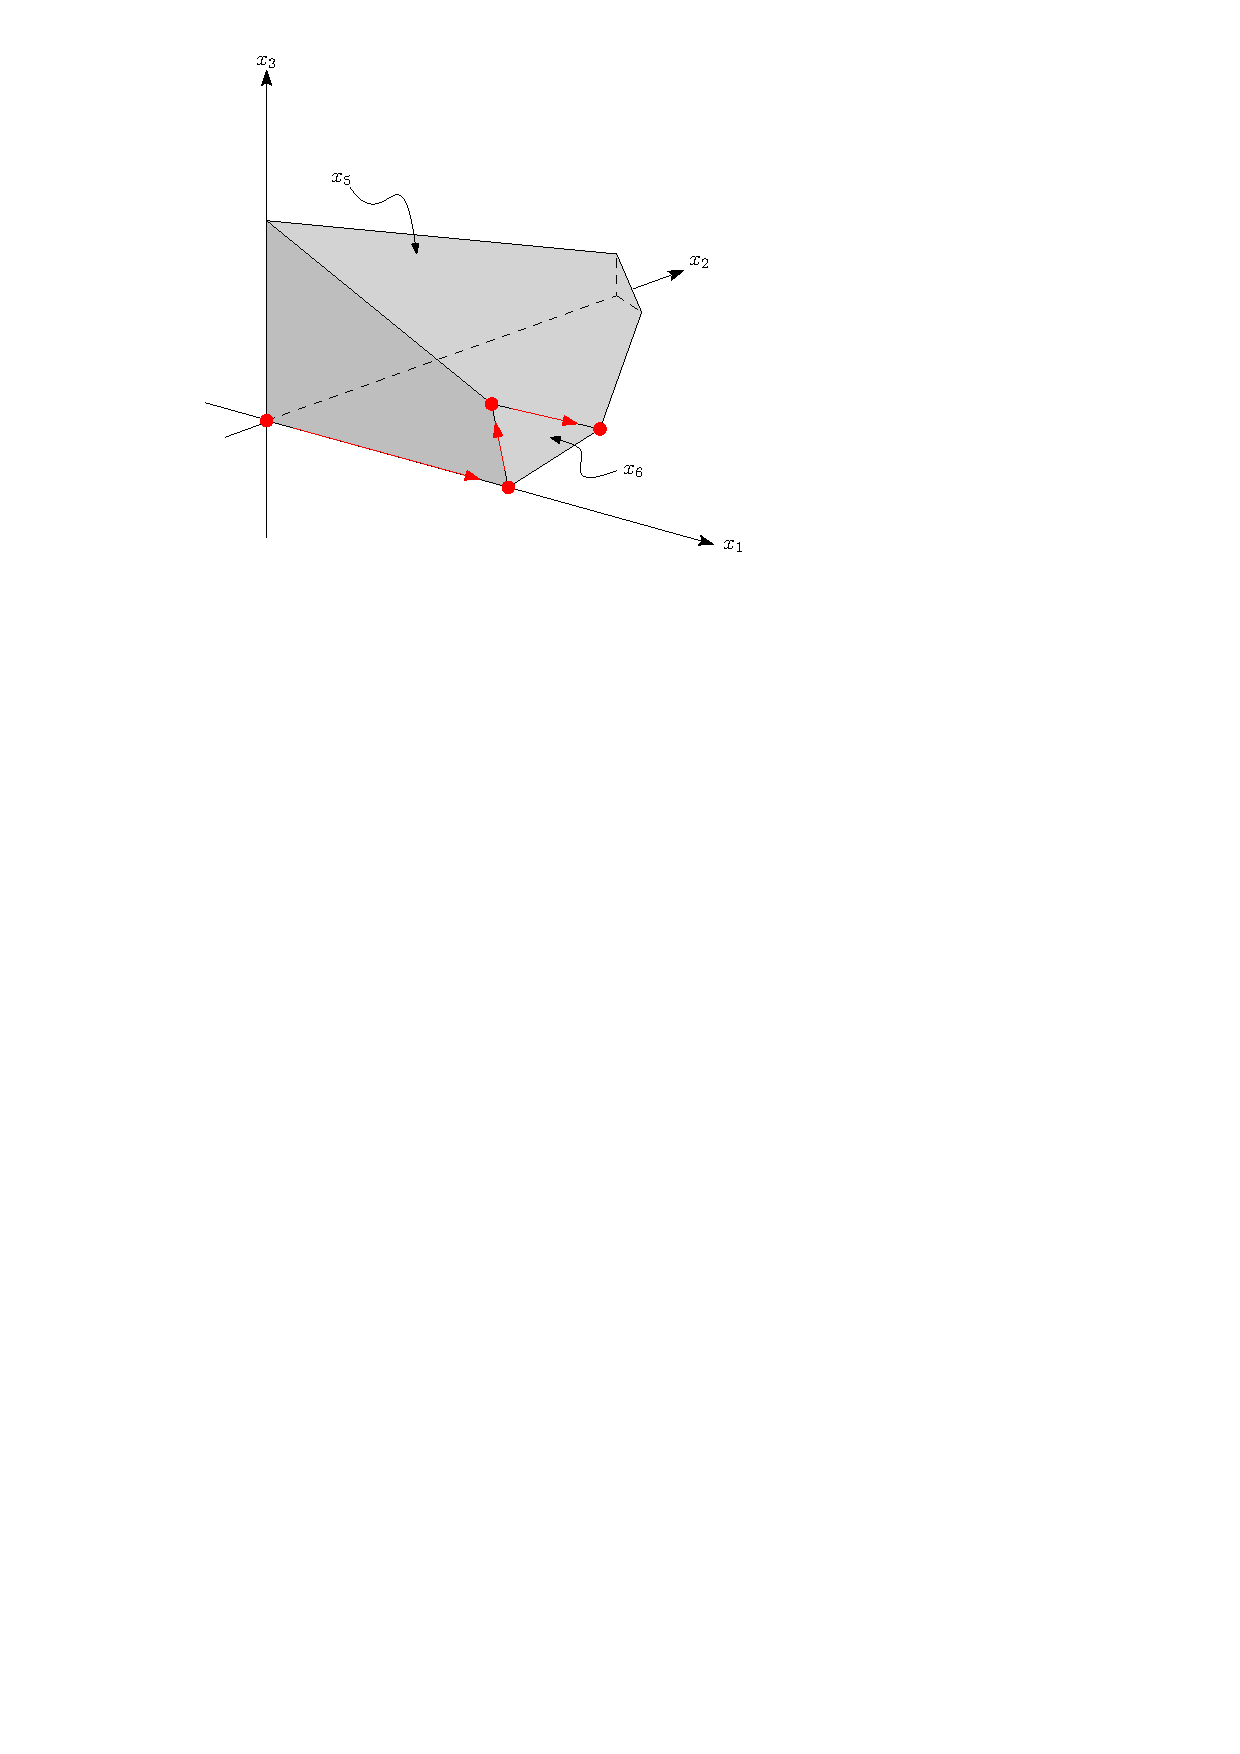
\includegraphics[width=0.4\linewidth]{lp/simplex-example-3d.pdf}
    \qquad\qquad
    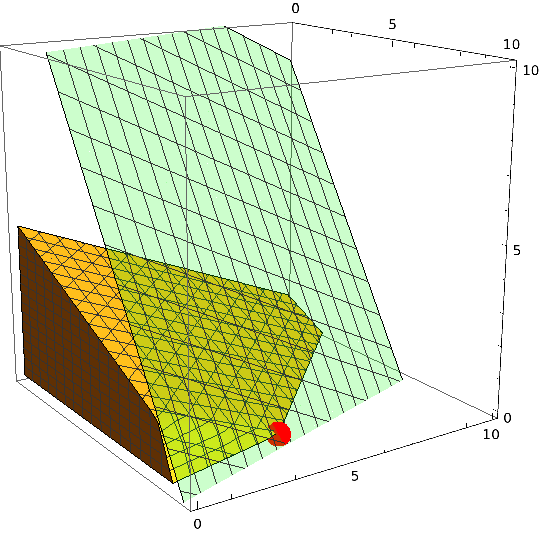
\includegraphics[width=0.4\linewidth]{lp/simplex-example-3d-2.pdf}
    \caption{Running the simplex algorithm on the example linear program. The figure on the right shows the feasible region in orange with the objective function as a green plane, and the optimum as a red dot in the graph.}
    \label{fig:simplex-example}
\end{figure}

\subsection{Implementing the Simplex Algorithm}

\begin{codebox}
    \Procname{$\proc{Simplex}(A,b,c)$}
    \li $(N,B,A,b,c,v) = \proc{Init-Simplex}(A,b,c)$ \RComment{init and convert to slack form}
    \li $\Delta = []$ \RComment{vector of length $m$}
    \li \While $\exists j \in N.\, c_j > 0$ \Do
        \li \Comment{break ties by choosing variable with smallest index}
        \li $e = \{e \in N \mid c_e > 0 \}[0]$
        \li \For $i \in B$ \Do
            \li \If $a_{ie} > 0$ \Then
                \li $\Delta_i = b_i/a_{ie}$
            \li \Else $\Delta_i = \infty$
            \End
        \End
        \li \Comment{find tightest constraint, break ties by choosing variable with smallest index}
        \li $l = \Argmin_{i \in B} \{ \Delta_i \}$
        \li \If $\Delta_i \isequal \infty$ \Then
            \li \Return unbounded
        \li \Else $(N,B,A,b,c,v) = \proc{Pivot}(N,B,A,b,c,v,l,e)$ \RComment{perform pivot}
        \End
    \End
    \li \For $i = 1$ \To $n$ \Do
        \li \If $i \in B$ \Then
            \li $\bar{x}_i = b_i$
        \li \Else $\bar{x}_i = 0$
        \End
    \End
    \li \Return $(\bar{x}_1,\ldots,\bar{x}_n)$
\end{codebox}

\subsection{Finding the Tightest Constraint} \index{minimum ratio test}

The tightest constraint can be easily identified using a method known as the \textit{\textbf{minimum ratio test}}. Once we have selected a non-basic variable as entering variable, say $x_e$, we iterate over the basic variables, and select the $i$th basic variable that minimizes $b_i/a_{ie}$ if $a_{ie}$ is negative. If $a_{ie}$ is positive, then the constraint does not limit how much we can increase $x_e$. In more concise notation, 
$$
l = \Argmin_{i \in \{b \in B \mid a_{be} > 0\}} \frac{b_i}{a_{ie}}.
$$
If there are multiple variables with the same smallest $b_i/a_{ie}$, we break ties by choosing the one with the smallest index. This rule is known as \textit{\textbf{Bland's rule}}. The overall idea of the minimum ratio test should be quite intuitive. Consider the expression of a basic variable with nonnegativity constraint of the form 
$$
x_i = b_i - a_{i1} x_1 - \cdots - a_{ie} x_e \geq 0
$$
$x_e$ is bounded by $b_i/a_{ie}$, so to find the tightest constraint on how much we can increase $x_e$, we want to minimize the ratio $b_i/a_{ie}$.

\section{Time Complexity of the Simplex Algorithm} \index{degeneracy (LP)} \index{Klee-Minty cube}

At any given point during the execution of the simplex algorithm, there are $m$ basic variables. It can be shown that the set $B$ of basic variables uniquely determines a slack form. There are $n+m$ variables. Hence, there are at most ${n+m \choose m}$ unique slack forms. If the algorithm terminates (which can be achieved using Bland's rule to prevent cycling), it terminates within ${n+m \choose m}$ iterations. Otherwise, it does not terminate and we say the algorithm \textit{\textbf{cycles}}. Cycling is usually due to \textit{\textbf{degeneracy}}, in which the simplex algorithm fails to change the objective value. Each iteration of the simplex algorithm takes $O(mn)$ time due to the \proc{Pivot} operation.

In the worst case, the simplex algorithm has a time complexity of $\Theta(2^d)$ where $d$ is the dimension of the feasible region, and Klee \& Minty proved the upper bound on worst-case time complexity and provided an example linear program, now known as the \textit{\textbf{Klee-Minty cube}} on which the algorithm runs in exponential time. However, in practice, the simplex algorithm is surprisingly efficient, and it often runs in polynomial time. It often beats asymptotically more efficient algorithms like the ellipsoid algorithm in practice. This phenomenon is explained by Spielman \& Teng in their paper, \textit{Smoothed Analysis of Algorithms: Why the Simplex Algorithm Usually Takes Polynomial Time}.

\chapter{Duality}
\section{Proving Optimality}

Given a maximization linear program, it is easy to show that the optimal objective value has a certain lower bound by providing a feasible solution that achieves the value. However, this is not sufficient for proving the upper bound of the given linear program. A single feasible solution is not enough because the optimal solution must be the maximum over all feasible solutions.

\section{Certificate of Optimality}

To obtain an upper bound, we can make a linear combination of the inequality constraints. For example, given this linear program
\begin{alignat*}{3}
    &\text{Maximize} \quad && x_1 + 6x_2 \\
    &\text{Subject to} \quad && x_1 &&\leq 200 \\
                    & &&  x_2 &&\leq 300 \\
                    & &&  x_1 + x_2 &&\leq 400 \\
                    & &&  x_1,x_2 &&\geq 0
\end{alignat*}
We claim that $(x_1,x_2) = (100, 300)$ is optimal with objective value 1900. If we take the second constraint multiplied by 5 and add it to the third constraint, we have
$$
5x_2 + (x_1+x_2) \leq 5 \cdot 300 + 400 = 1900
$$
This shows that no feasible solution can beat 1900 -- an upper bound.

More generally, we introduce variables $y_1,y_2,\ldots$ by which we will be multiplying the constraints. Using the previous example, we have
\begin{alignat*}{3}
    &\textbf{Multiplier} \quad && \textbf{Inequality} \\
    & y_1 \quad && x_1 &&\leq 200 \\
    & y_2 \quad &&  x_2 &&\leq 300 \\
    & y_3 \quad && x_1 + x_2 &&\leq 400 \\
\end{alignat*}
After multiplying the constraints by the factors, we have
$$
(y_1+y_3)x_1 + (y_2 + y_3)x_2 \leq 200 y_1 + 300 y_2 + 400 y_3
$$
And we want
\begin{itemize}
    \item $y_1,y_2,y_3 \geq 0$ because otherwise the direction of inequalities flips, and
    \item the left-hand side to be an upper bound on the objective $x_1 + 6x_2$.
\end{itemize}

In this specific example, we want
\begin{itemize}
    \item $y_1,y_2,y_3 \geq 0$, and
    \item $y_1 + y_3 \geq 1$ and $y_2 + y_3 \geq 6$.
\end{itemize}
But this is just \textit{\textbf{another linear program}}! Namely,
\begin{alignat*}{3}
    &\text{Minimize} \quad && 200y_1 + 300y_2 + 400y_3 \\
    &\text{Subject to} \quad && y_1 + y_3 &&\geq 1 \\
                    & &&  y_2 + y_3 &&\geq 6 \\
                    & &&  y_1,y_2+y_3 &&\geq 0
\end{alignat*}

\index{dual} \index{primal}
This linear program is called the \textit{\textbf{dual}}, while the original linear program is called the \textit{\textbf{primal}}.

If we can find a specific optimal solution to the dual program for which the objective function is equal to the primal objective, then we can conclude that the given primal solution is indeed optimal.

\chapter{Linear Programming Applications}
\section{Network Flow via LP}

Flow $f$ is valid if:
\begin{itemize}
    \item capacity constraints
    \item flow conservation
\end{itemize}
are satisfied.

This can be framed as a linear programming problem that


\chapter{Integer Programming}

\chapter{Ellipsoid Algorithm for LP}

\part{Approximation Algorithms}

\chapter{Approximation}
\section{Why Approximation?}

As we have seen in the last part, many problems of both theoretical and practical interest turn out to be NP-complete. And it is strongly believed that it is unlikely to have polynomial time algorithms to solve such problems. That's why we are interested in approximation algorithms. Instead of solving the problems exactly, we can approximate the results. In some other cases, we may want to use an approximation algorithm even if a polynomial-time exact algorithm exists for that particular problem.

\section{Approximation Ratio}

The objective of approximation algorithm is to \textit{\textbf{maximize ``profit''}} (in a maximization problem) or \textit{\textbf{minimize ``cost''}} (in a minimization problem). We use the notion of approximation ratio to measure how good or bad an approximation algorithm is.

\begin{definition}[Approximation Ratio] \index{approximation ratio}
    Given a problem instance $I$, let $\mathrm{ALG}(I)$ be the solution returned by the approximation algorithm and let $\mathrm{OPT}(I)$ be some optimal solution. Then, for a maximization problem, we define the \textit{\textbf{approximation ratio}} as
    $$
    \frac{\mathit{Profit}(\mathrm{OPT}(I))}{\mathit{Profit}(\mathrm{ALG}(I))}
    $$
    Similarly, for a minimization problem we define the approximation ratio as
    $$
    \frac{\mathit{Cost}(\mathrm{ALG}(I))}{\mathit{Cost}(\mathrm{OPT}(I))}
    $$
    We also define the asymptotic approximation ratio as
    $$
    \lim_{\mathit{Cost}(\mathrm{OPT}(I)) \to \infty}\frac{\mathit{Cost}(\mathrm{ALG}(I))}{\mathit{Cost}(\mathrm{OPT}(I))} \qquad \text{or} \qquad \lim_{\mathit{Profit}(\mathrm{OPT}(I)) \to \infty} \frac{\mathit{Profit}(\mathrm{OPT}(I))}{\mathit{Profit}(\mathrm{ALG}(I))}
    $$
\end{definition}

\begin{definition}[c-Approximation]
    For a minimization problem, we say an algorithm ALG is a $c$-approximation if
    $$
    \mathit{Cost}(\mathrm{ALG}(I)) \leq c \cdot \mathit{Cost}(\mathrm{OPT}(I))
    $$
    For a maximization, we say ALG is a $c$-approximation if
    $$
    \mathit{Profit}(\mathrm{ALG}(I)) \geq \frac{1}{c} \mathit{Profit}(\mathrm{OPT}(I))
    $$
\end{definition}

Note that for all approximation algorithms, we should have $c \geq 1$. In the context of a minimization problem, this means the approxmation ratios are always such that $c \geq 1$. In maximization problem, approximation ratios are a fraction of the optimal profit.

\section{Classes of Approximation Schemes} \index{FPTAS} \index{PTAS}

An \textbf{FPTAS} (\textit{\textbf{fully polynomial time approximation scheme}}) is a $(1+\epsilon)$-approximation algorithm using time polynomial in the input size and $1/\epsilon$.

A \textbf{PTAS} (\textit{\textbf{polynomial time approximation scheme}}) is a $(1+\epsilon)$-approximation algorithm using time polynomial in the input size. A PTAS may not be polynomial in terms of $1/\epsilon$.

\chapter{Greedy Approximation Algorithms}
\section{Makespan}

\textbf{Input}: Given $m$ identical machines, $n$ jobs. Job $j$ requires processing time $t_j$.

\textbf{Output}: Assignment jobs to machines to minimize makespan.

More formally, let $S[i]$ be the set of jobs assigned to machine $i$ in a solution. Each job must run contiguously on one machine, and each machine can process at most one job at a time. We define the load on a machine $i$ as $L_i = \sum_{j \in S[i]}t_j$. The objective is to minimize the maximum load, i.e. $\max_i L_i$.

The makespan is one of the most well-studied problem for approximation and online algorithms. The analyses of the makespan problem and associated approximation algorithms were first done by Graham in the 60s, and Graham's studies on approximation algorithms are considered the first ones that formally studied the worst case performance of approximation algorithms.

\subsection{Makespan is NP-Hard} \index{makespan problem}

By reduction from PARTITION. The PARTITION problem is defined as follows:

Given $A = \{a_1,a_2,\ldots,a_n\}$, is there a partition of $A$ into $A_1 \cup A_2$ such that $\sum_{a_i \in A_1} = \sum_{a_j \in A_2}$. It can be shown that SUBSET-SUM $\leq_p$ PARTITION and hence PARTITION is $\mathsf{NP}$-complete. 

\subsection{Greedy Approximation Algorithm for Makespan} \index{online algorithm}

We will use a greedy approximation algorithm to solve the makespan problem. For the greedy algorithm, we consider the jobs at an arbitrary order and assign each job to the machine with smallest load at the time. This is an example of an \textit{\textbf{online algorithm}} because it looks at jobs as they arrive. The following theorem states that the online greedy algorithm gives a solution that is at most twice as bad.

\begin{theorem}
    Regardless of the order, greedy gives a 2-approximation.
\end{theorem}

\begin{proof}
    Suppose machine $i$ is the bottleneck under greedy so $L=L_i$. Let $j'$ be the last job scheduled on machine $i$ by greedy. Immediately before $j'$ was assigned to $i$, $i$ has the smallest load. Load of the other machines could have only increased from then, so $L_i - t_{j'} \leq L_k$ for all $k$. Take the average over all $k$, $L_i - t_{j'} \leq 1/m \sum_{j} t_j$. Observe that $L_{opt} \geq \Argmax_j t_j$ and $L_{opt} \geq 1/m \sum_{j} t_j$. Then,
    $$
    L_i \leq t_{j'} + \frac{1}{m} \sum_{j} t_j \leq L_{opt} + L_{opt} = 2L_{opt}
    $$
\end{proof}

The time complexity of this online algorithm is $O(n \log m)$ since we can use a priority queue to keep track of the least loaded machine. The approximation ratio of 2 that we proved earlier is, in fact, not tight. We can show a marginally better approximation ratio as follows.

\begin{corollary}
    Regardless of the order, greedy gives a $(2-\frac{1}{m})$ approximation. This approximation ratio is tight.
\end{corollary}

\begin{proof}
    One can simply average over $k \neq i$ instead of all $k$ and show that the approximation ratio is $(2-\frac{1}{m})$. To show that the ratio is tight, consider $m(m-1)$ jobs of length 1 followed by one job of length $m$. Greedy evenly distributes unit length jobs on all $m$ machines, and assigning the last heavy job, resulting in a makespan of $L = m-1+m = 2m-1$. On the other hand, the optimal makespan $L_{opt} = m$ evenly distributes unit length jobs among $m-1$ machine and puts the single heavy job on the remaining one machine.
\end{proof}

This input construction resulting in $2m-1$ makespan suggests that it is probably a bad idea to keep the job with the longest processing time until the end, and indeed, we can achieve a better approximation ratio if we consider the job with the longest processing time first.

\index{Graham's longest processing time-first algorithm}
If we are given all the jobs, we can have an offline algorithm that gives a better approximation. This is the \textit{\textbf{Graham's longest processing time-frist (LPT) algorithm}}. It uses the same greedy approach of assigning jobs to the least loaded machine, but instead of considering jobs in an arbitrary, we consider them in a non-decreasing order of processing time, namely $t_1 \geq t_2 \geq \ldots \geq t_n$.

\begin{theorem}
    Graham's LPT algorithm gives a $3/2$-approximation. 
\end{theorem}

\begin{proof}
    Suppose machine $i$ is the bottleneck and job $j'$ is the last job scheduled on machine $i$. We consider the following two cases:

    Case 1: Machine $i$ has only one job, $j'$. In this case, the greedy solution is optimal because $L = L_i = t_{j'}$ and some machine has to take job $j'$. This gives us an 1-approximation.

    Case 2: Machine $i$ has at least two jobs. Then, there must be more tasks than the number of machines, so $n \geq m+1$. We claim that if there are more than $m$ total jobs, then $L_{opt} \geq 2 t_{m+1}$. To see why, recall that the input is ordered so that the first $m+1$ jobs have processing time of at least $t_{m+1}$ and by the Pigeonhole Principle, the optimal solution has to put at least two of them on the same machine, so the optimal makespan must also be at least as large as the load on that machine. Going back to Case 2, it must be the case that $t_{j'} \leq t_{m+1}$. Then,
    $$
    L = L_i = (L_i - t_{j'}) + t_{j'} \leq L_{opt} + \frac{1}{2} L_{opt} = \frac{3}{2}L_{opt}
    $$
    Since $t_{j'} \leq t_{m+1} \leq 1/2 L_{opt}$.
\end{proof}

There is a tighter bound on the approximation ratio proved by Graham.

\begin{theorem}[Graham 1966]
    Greedy LPT achieves a $(\frac{4}{3} - \frac{1}{3m})$-approximation, and this approximation ratio is tight.
\end{theorem}

\begin{proof}
    TODO
\end{proof}

\section{Vertex Cover}

\textbf{Input}: An undirected graph $V = (V,E)$.

\textbf{Output}: Vertex cover $C$ of minimum cardinality. Recall that $C$ is a vertex cover if every edge has at least one of its two endpoints in $C$.

We have shown that VERTEX-COVER is $\mathsf{NP}$-complete.

\section{Greedy Approximation Algorithm for Vertex Cover}

Naturally, we will consider the greedy approach when trying to come up with an approximation algorithm for the vertex cover problem. To begin with, let's try picking the edges arbitrarily, without any particular ordering.

\begin{codebox}
    \Procname{$\proc{Approx-Vertex-Cover}(G=(V,E))$}
    \li $C = \emptyset$
    \li $E' = E$
    \li $M = \emptyset$ 
    \li \While $E' \neq \emptyset$ \Do
        \li pick $\{u,v\} \in E'$
        \li $C = C \cup \{u,v\}$ 
        \li $M = M \cup \{\{u,v\}\}$ 
        \li \textbf{remove} $\{u,v\}$ from $E'$ 
        \li \textbf{remove} all edges incident on $u$ or $v$
\end{codebox}

In addition to the vertex cover $C$, the algorithm also computes $M$, which we call the maximal matching.

\begin{theorem}
    \proc{Approx-Vertex-Cover} gives a 2-approximation.
\end{theorem}

\begin{proof}
    Let $M$ be the maximal matching returned by the greedy approximation algorithm, and let $S$ be the vertex cover returned by greedy. Let $C_{opt}$ be the optimal vertex cover.
\end{proof}

\chapter{Local Search}
\section{Oblivious and Non-Oblivious Local Search} \index{Ford-Fulkerson method} \index{gradient descent} \index{oblivious local search} \index{non-oblivious local search}

The idea behind the local search heuristic is to start with a feasible solution and search for a local optimum. In some cases, this approach can actually generate a global optimal solution. The \textit{\textbf{Ford-Fulkerson method}} for max flow is an example of a local search algorithm that yields a globally optimal solution. The issue with local search is that we might get stuck at a bad local optimum. And indeed, in some other cases, local search does not guarantee a global optimal, but even if this is the case, it might still give us a good approximation. A famous example of this approach is the \textit{\textbf{gradient descent}} algorithm, commonly used in machine learning and convex optimization. Gradient descent can be further improved by initializing the starting position randomly, giving us the stochastic gradient descent algorithm.

For optimization problems, we are often given an objective function to optimize (maximize or minimize). We can use local search to incrementally improve our solution with respect to the global optimum of the objective function. This approach is called \textit{\textbf{oblivious local search}}. Alternatively, we might want to optimize a potential function (think this as a surrogate for the actual objective function). This is called \textit{\textbf{non-oblivious local search}}. The Ford-Fulkerson algorithm is an example of a non-oblivious local search algorithm, where we optimize the flow in a residue network as opposed to the original flow network.

\section{Exact Max-k-SAT}

\textbf{Input}: An exact $k$-CNF formula $\phi = C_1 \land C_2 \land \cdots \land C_m$ where each clause $C_i$ has exactly $k$ literals, and a weight $w_i \geq 0$ associated with each clause $C_i$.

\textbf{Output}: A truth assignment $\tau$ maximizing the total weight of clauses satisfied under $\tau$.

Let $W(\tau)$ be the total weight of $\phi$ given the truth assignment $\tau$, which is defined to be the weighted sum of all clauses satisfied by $\tau$. That is, $W(\tau) = \sum \{w_i \mid \text{$C_i$ is satisfied under $\tau$ }\}$. 

\section{Local Search Algorithm for Exact Max-k-SAT}

We define the local neighborhood $N_d(\tau)$ for a truth assignment $\tau$ as
$$
N_d(\tau) = \{ \tau' \mid \text{$\tau$ and $\tau'$ differs on at most $d$ variables}\}
$$
Naturally, we have the followng local search approximation algorithm.

\begin{codebox}
    \Procname{$\proc{Local-Search-Approx}(\phi)$}
    \li $\tau = \text{arbitrary initial assignment}$
    \li \While $\exists \tau' \in N_d(\tau).\, W(\tau') > W(\tau)$ \Do
        \li $\tau = \tau'$ 
\end{codebox}

Let us first analyze the approximation ratio for the case when we fix $d=1$.

\begin{theorem}
    The local search with $d=1$ gives a $2/3$-approximation to the exact max-2-SAT problem. 
\end{theorem}

\begin{proof}
    Let $\tau$ be a local optimum. Further, let
    \begin{itemize}
        \item $S_0 =$ set of clauses not satisfied under $\tau$ 
        \item $S_1 =$ set of clauses from which exactly one literal is true under $\tau$ 
        \item $S_2 =$ set of clauses from which both literals are true under $\tau$
        \item $W_0,W_1,W_2$ be the corresponding total weights
    \end{itemize}
    We say 
\end{proof}

\part{Randomized Algorithms}

\chapter{Randomization}
\section{Bounding Probability}

Union bound:
$$
\Prob(A \cup B) \leq \Prob(A) + \Prob(B)
$$

\begin{proof}
    $\Prob(A \cup B) = \Prob(A) + \Prob(B) - \Prob(A \cap B) \leq \Prob(A) + \Prob(B)$
\end{proof}

Chebyshev's inequality: for $k > 0$
$$
\Prob(|X-\Expected(X)| \geq a \sigma) \leq \frac{1}{a^2}
$$
where $\sigma^2 = \Var(X)$ or equivalently
$$
\Prob(|X-\Expected(X)| \geq a) \leq \frac{\Var(X)}{a^2}
$$

Markov's inequality: for nonnegative random variable $X$ and $a>0$,
$$
\Prob(X \geq a) \leq \frac{\Expected(X)}{a}
$$

Chernoff bound:
$$
\Prob(X \geq a) = \Prob(e^{tX} \geq e^{ta}) \leq \frac{\Expected(e^{tX})}{e^{ta}}
$$
If $X = \sum_{i=1}^n X_i$ and $\Expected(X) \leq \mu$,
$$
\Prob(X \geq (1+\delta)\mu) \leq \left( \frac{e^\delta}{(1+\delta)^{1+\delta}} \right)^{\mu} 
$$ 

\part{Algorithms on Strings}

%----------------------------------------------------------------------------------------
%	APPENDIX
%----------------------------------------------------------------------------------------
\part*{Appendix}
\appendix
\chapter*{Commonly Used Axioms \& Theorems}
\addcontentsline{toc}{chapter}{\textcolor{ocre}{Axioms \& Theorems}} 

\renewcommand{\leftmark}{\sffamily\bfseries Axioms \& Theorems}
\renewcommand{\rightmark}{\sffamily\bfseries Axioms \& Theorems}

\section*{Rules of Inference} \label{rulesofinference}

\begin{axiom_appendix}[Modus Ponens]
$(P \wedge (P \implies Q)) \implies Q $
\end{axiom_appendix}

\begin{axiom_appendix}[Modus Tollens]
$(\neg Q \wedge (P \implies Q)) \implies \neg P $
\end{axiom_appendix}

\begin{axiom_appendix}[Hypothetical Syllogism (transitivity)]
\hfill

$((P \implies Q) \wedge (Q \implies R)) \implies (P \implies R) $
\end{axiom_appendix}

\begin{axiom_appendix}[Disjunctive Syllogism]
$((P \vee Q) \wedge \neg P) \implies Q$
\end{axiom_appendix}

\begin{axiom_appendix}[Addition]
$P \implies (P \vee Q)$
\end{axiom_appendix}

\begin{axiom_appendix}[Simplification]
$(P \wedge Q) \implies P$
\end{axiom_appendix}

\begin{axiom_appendix}[Conjunction]
$((P) \wedge (Q)) \implies (P \wedge Q)$
\end{axiom_appendix}

\begin{axiom_appendix}[Resolution]
$((P \vee Q) \wedge (\neg P \vee R)) \implies (Q \vee R)$
\end{axiom_appendix}

\section*{Laws of Logic}

\begin{axiom_appendix}[Implication Law]
$(P \implies Q) \equiv (\neg P \vee Q)$
\end{axiom_appendix}

\begin{axiom_appendix}[Distributive Law]
\begin{align*}
    (P \wedge (Q \vee R)) &\equiv ((P \wedge Q) \vee (P \wedge R)) \\
    (P \vee (Q \wedge R)) &\equiv ((P \vee Q) \wedge (P \vee R))
\end{align*}
\end{axiom_appendix}

\begin{axiom_appendix}[De Morgan's Law]
\begin{align*}
    \neg (P \wedge Q) &\equiv (\neg P \vee \neg Q) \\
    \neg (P \vee Q) &\equiv (\neg P \wedge \neg Q)
\end{align*}
\end{axiom_appendix}

\begin{axiom_appendix}[Absorption Law]
\begin{align*}
    (P \vee (P \wedge Q)) &\equiv P \\
    (P \wedge (P \vee Q)) &\equiv P
\end{align*}
\end{axiom_appendix}

\begin{axiom_appendix}[Commutativity of AND]
$A \wedge B \equiv B \wedge A$
\end{axiom_appendix}

\begin{axiom_appendix}[Associativity of AND]
$(A \wedge B) \wedge C \equiv A \wedge (B \wedge C)$
\end{axiom_appendix}

\begin{axiom_appendix}[Identity of AND]
$\textbf{T} \wedge A \equiv A$
\end{axiom_appendix}

\begin{axiom_appendix}[Zero of AND]
$\textbf{F} \wedge A \equiv \textbf{F}$
\end{axiom_appendix}

\begin{axiom_appendix}[Idempotence for AND]
$A \wedge A \equiv A$
\end{axiom_appendix}

\begin{axiom_appendix}[Contradiction for AND]
$A \wedge \neg A \equiv \textbf{F}$
\end{axiom_appendix}

\begin{axiom_appendix}[Double Negation]
$\neg (\neg A) \equiv A$
\end{axiom_appendix}

\begin{axiom_appendix}[Validity for OR]
$A \vee \neg A \equiv \textbf{T}$
\end{axiom_appendix}

\section*{Induction}

\vspace{\parskip}

\begin{axiom_appendix}[Well Ordering Principle]
Every nonempty set of nonnegative integers has a smallest element. i.e., For any $A \subset \N$ such that $A \neq \emptyset$, there is some $a \in A$ such that $\forall a' \in A.a\leq a'$.
\end{axiom_appendix}

\section*{Recurrences}

\vspace{\parskip}

\begin{theorem_appendix}[The Master Theorem]
Suppose that for $n \in \Z^+$.
\begin{equation*}
    T(n) =
    \begin{cases}
    c & \text{if $n<B$} \\
    a_1 T(\lceil n/b \rceil) + a_2 T(\lfloor n/b \rfloor) + dn^i & \text{if $n\geq B$}
    \end{cases}
\end{equation*}
where $a_1, a_2, B, b \in \N$.

Let $a = a_1+a_2 \geq 1$, $b>1$, and $c,d,i \in \R \cup \{0\}$. Then,
\begin{equation*}
    T(n) \in
    \begin{cases}
    O(n^i \log n) & \text{if $a=b^i$} \\
    O(n^i) & \text{if $a < b^i$} \\
    O(n^{\log_b a}) & \text{if $a > b^i$}
    \end{cases}
\end{equation*}
\end{theorem_appendix}

Linear Recurrences:

A linear recurrence is an equation
$$
f(n) = \underbrace{a_1 f(n-1) + a_2 f(n-2) + \cdots + a_d f(n-d)}_{\text{homogeneous part}}  + \underbrace{g(n)}_{\text{inhomogeneous part}}
$$
along with some boundary conditions.

The procedure for solving linear recurrences are as follows:

\begin{enumerate}
    \item Find the roots of the characteristic equation. Linear recurrences usually have exponential solutions (such as $x^n$). Such solution is called the \textbf{homogeneous solution}.
    $$
    x^n = a_1 x^{n-1} + a_2 x^{n-2} + \cdots + a_{k-1} x + a_k
    $$
    \item Write down the homogeneous solution. Each root generates one term and the homogeneous solution is their sum. A non-repeated root $r$ generates the term $cr^n$, where $c$ is a constant to be determined later. A root with $r$ with multiplicity $k$ generates the terms
    $$
    d_1r^n \quad d_2nr^n \quad d_3n^2r^n \quad \cdots \quad d_kn^{k-1}r^n
    $$
    where $d_1,\cdots,d_k$ are constants to be determined later.
    \item Find a \textbf{particular solution} for the full recurrence including the inhomogeneous part, but without considering the boundary conditions.
    
    If $g(n)$ is a constant or a polynomial, try a polynomial of the same degree, then of one higher degree, then two higher. If $g(n)$ is exponential in the form $g(n) = k^n$, then try $f(n) = ck^n$, then $f(n) = (bn+c)k^n$, then $f(n) = (an^2+bn+c)k^n$, etc.
    
    \item Write the \textbf{general solution}, which is the sum of homogeneous solution and particular solution.
    \item Substitute the boundary condition into the general solution. Each boundary condition gives a linear equation. Solve such system of linear equations for the values of the constants to make the solution consistent with the boundary conditions.
\end{enumerate}


\chapter*{Basic Prerequisite Mathematics}
\addcontentsline{toc}{chapter}{\textcolor{ocre}{Basic Prerequisite Mathematics}}
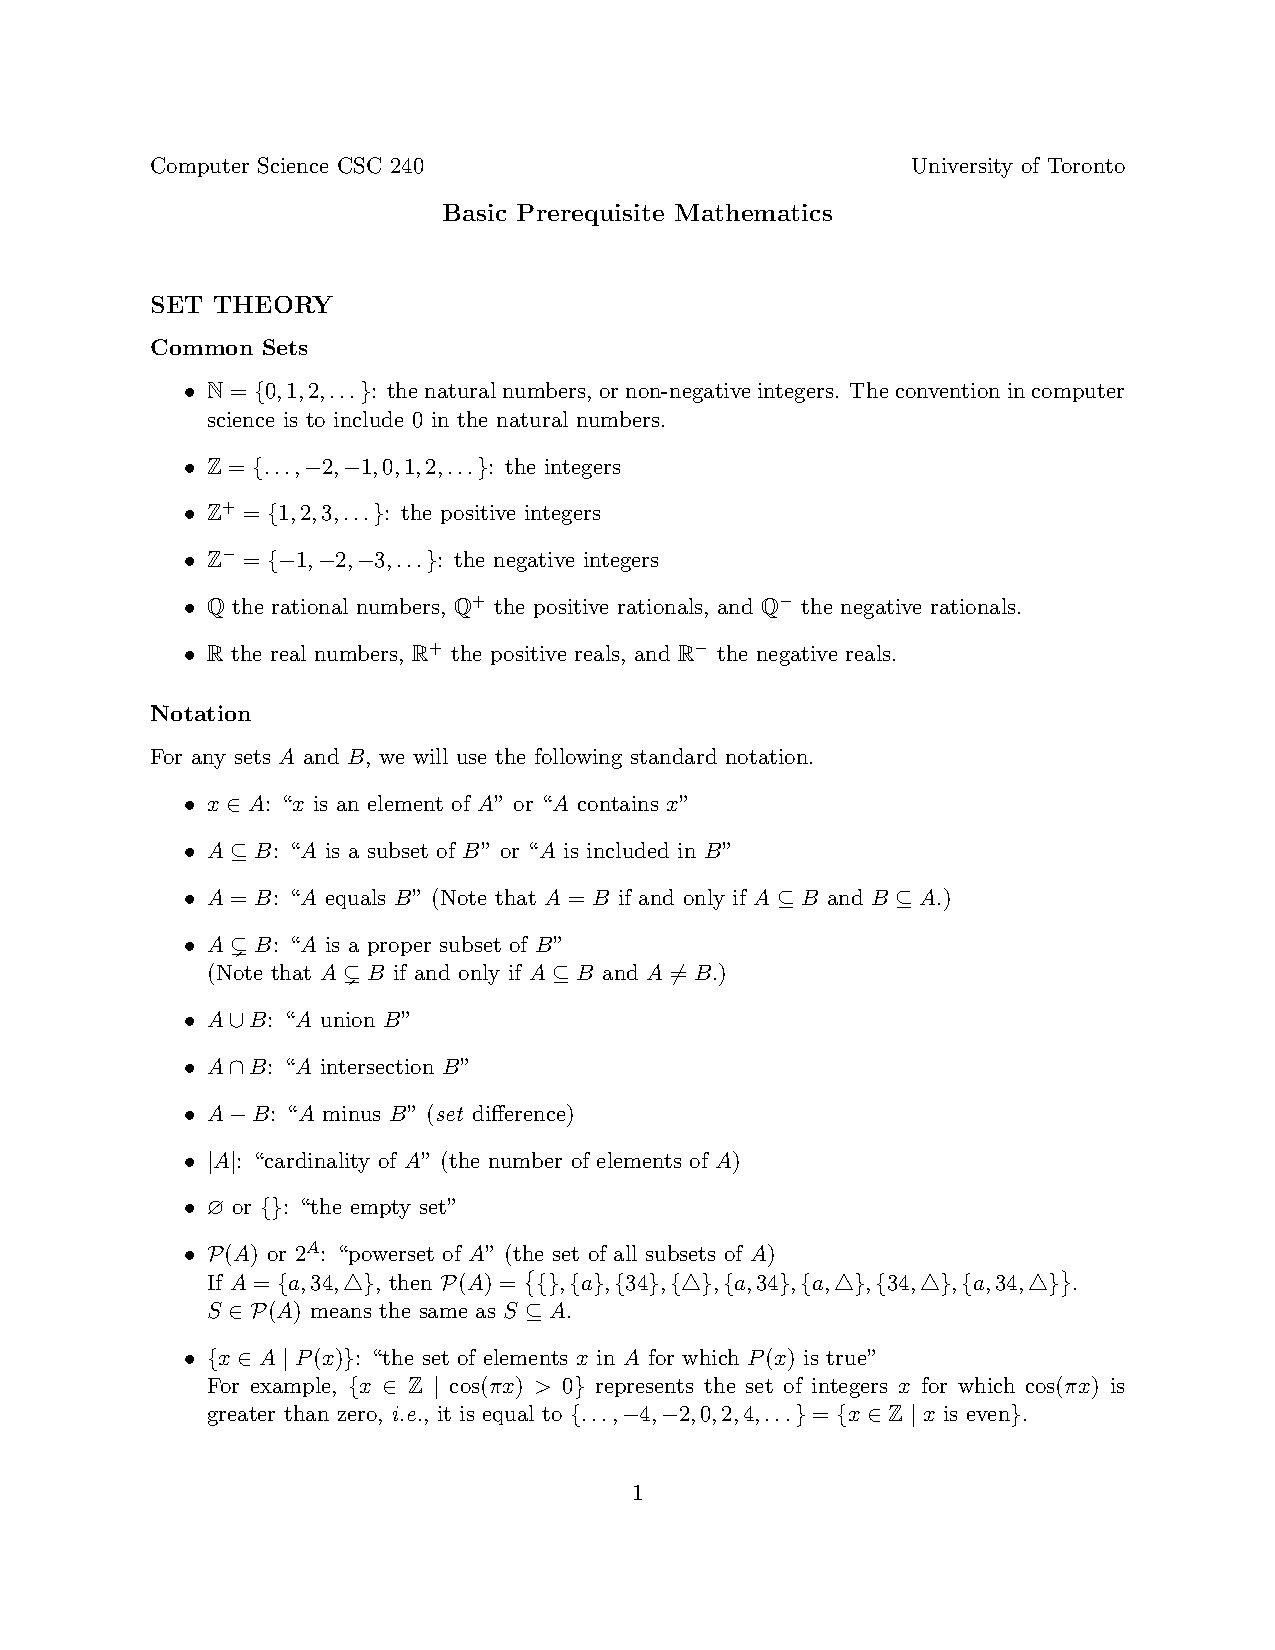
\includepdf[pages=-]{appendix/basicMath.pdf}

\chapter*{Proof Templates}
\addcontentsline{toc}{chapter}{\textcolor{ocre}{Proof Templates}}
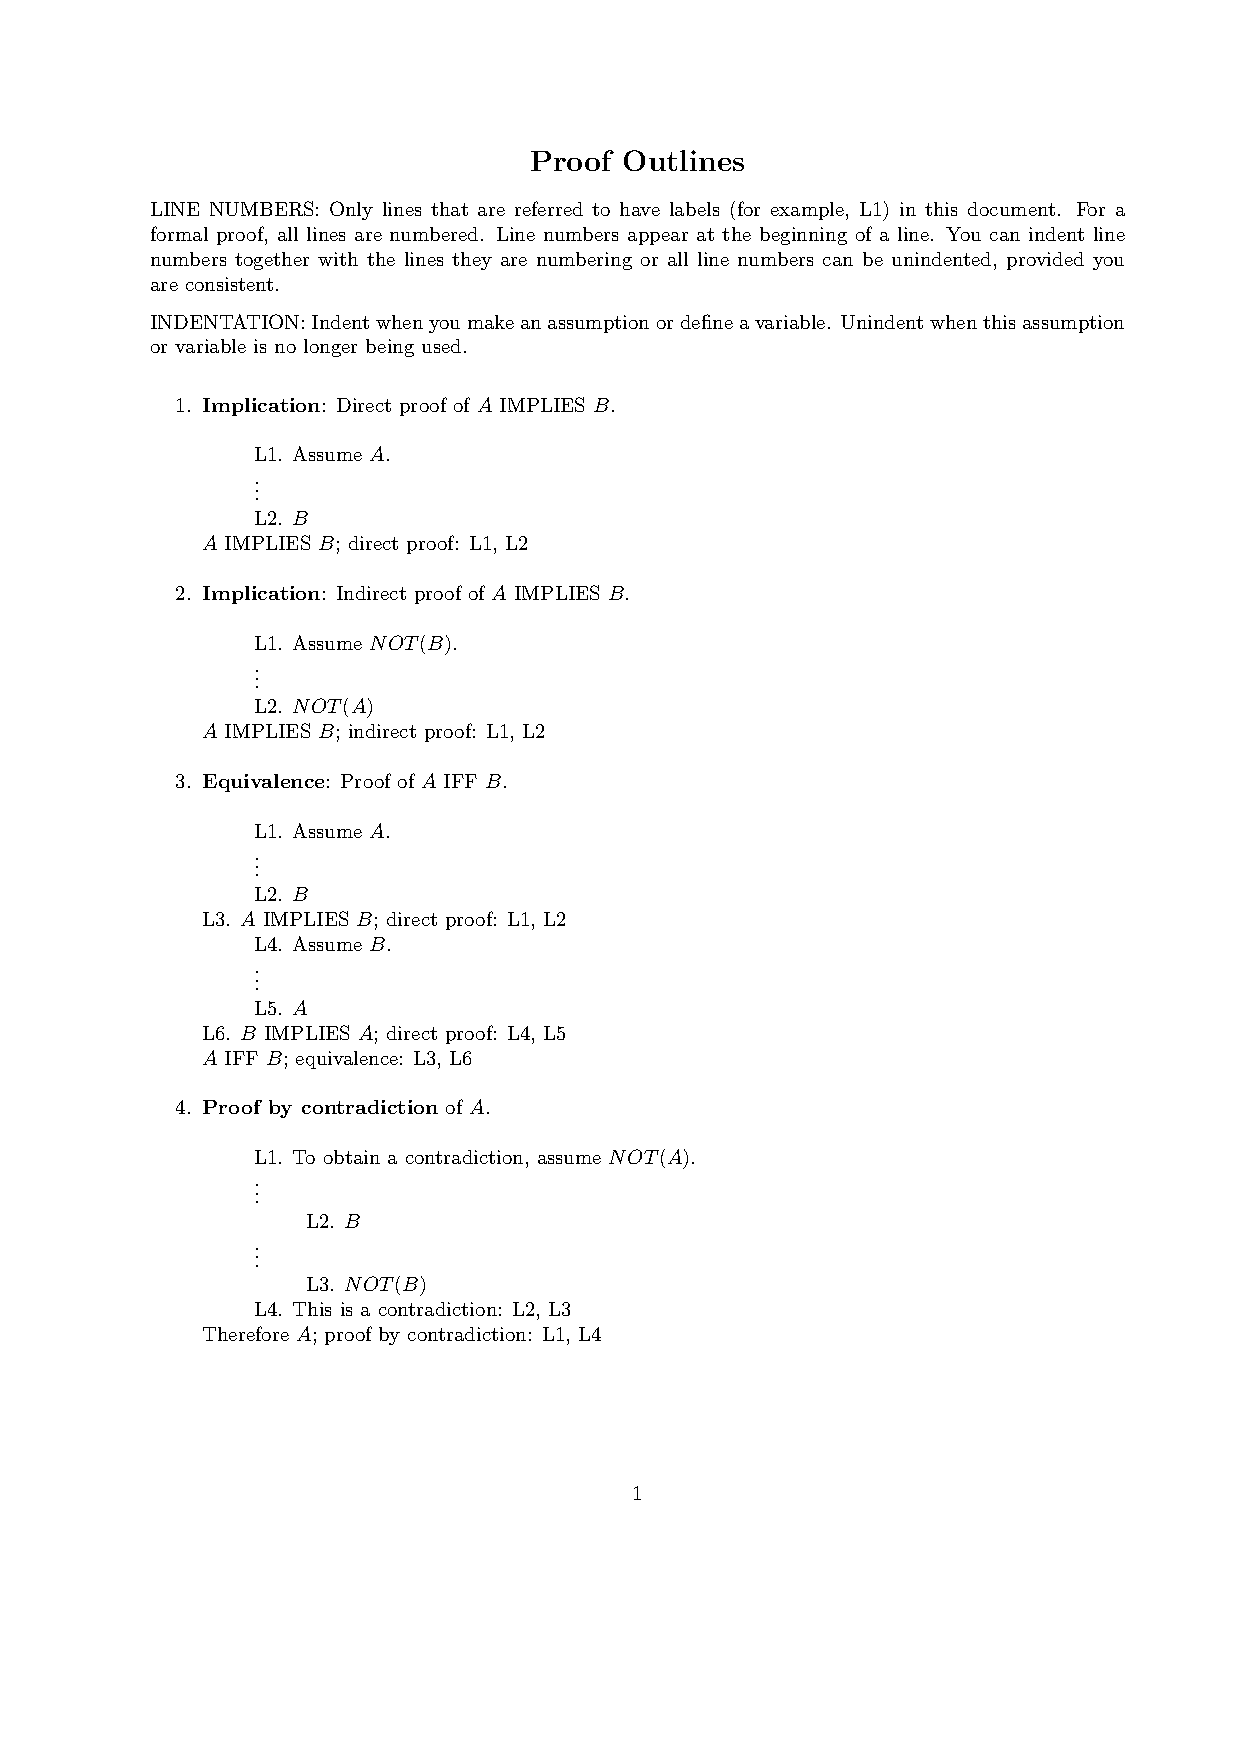
\includepdf[pages=-]{appendix/proofOutlines.pdf}

%----------------------------------------------------------------------------------------
%	INDEX
%----------------------------------------------------------------------------------------

\chapter*{Index}
\renewcommand{\leftmark}{\sffamily\bfseries Index}
\renewcommand{\rightmark}{\sffamily\bfseries Index}
%\cleardoublepage % Make sure the index starts on an odd (right side) page
\setlength{\columnsep}{0.75cm} % Space between the 2 columns of the index
\addcontentsline{toc}{chapter}{\textcolor{ocre}{Index}} % Add an Index heading to the table of contents

\printindex % Output the index

%------------------------------------------------
%   BIBLIOGRAPHY ENTRIES
%------------------------------------------------
\chapter*{Bibliography}
\renewcommand{\leftmark}{\sffamily\bfseries Bibliography}
\renewcommand{\rightmark}{\sffamily\bfseries Bibliography}
\addcontentsline{toc}{chapter}{\textcolor{ocre}{Bibliography}} % Add a Bibliography heading to the table of contents

\section*{Courses}
\addcontentsline{toc}{section}{Courses}
\printbibliography[heading=bibempty,type=misc]

\section*{Books}
\addcontentsline{toc}{section}{Books}
\printbibliography[heading=bibempty,type=book]

\section*{Journal Articles}
\addcontentsline{toc}{section}{Journal Articles}
\printbibliography[heading=bibempty,type=article]

\newpage

%------------------------------------------------
%   TUTORIALS
%------------------------------------------------

%----------------------------------------------------------------------------------------

\end{document}
